\section{TRIỂN KHAI, KIỂM THỬ VÀ ĐÁNH GIÁ}\label{sec:trien_khai_danh_gia}

Chương này trình bày quá trình hiện thực mô hình đã thiết kế ở Chương~\ref{sec:mo_hinh_de_xuat} trên EVE-NG, các vấn đề kỹ thuật phát sinh cùng nguyên nhân gốc và cách khắc phục, kết quả kiểm thử và đánh giá. Kết quả được phân thành ba mức: \textit{Đạt} khi có bằng chứng từ trạng thái thiết bị hoặc phép thử thực tế; \textit{Đạt một phần} khi chức năng hoạt động ở điều kiện bình thường nhưng còn tình huống chưa đáp ứng; và \textit{Chưa nghiệm thu} khi đã cấu hình nhưng chưa có phép thử đầu--cuối tương ứng.

\subsection{Phương pháp triển khai và kiểm thử}

Việc triển khai tuân theo các nguyên tắc:
\begin{itemize}
    \item Địa chỉ, VLAN, Site-ID, System-IP và ánh xạ cổng thống nhất giữa tài liệu thiết kế, topology EVE-NG và cấu hình thiết bị; mỗi thiết bị có một tệp cấu hình nguồn được quản lý phiên bản bằng Git và được đối chiếu lại với cấu hình đang chạy.
    \item Triển khai từ dưới lên: underlay trước overlay, hạ tầng trước dịch vụ, kết nối trước chính sách.
    \item Kiểm thử và chẩn đoán theo lớp: vật lý/liên kết $\rightarrow$ lớp 2 (VLAN, trunk, vòng lặp) $\rightarrow$ lớp 3 (gateway, tuyến, BGP/OSPF) $\rightarrow$ dịch vụ (DHCP, kết nối điều khiển) $\rightarrow$ ứng dụng. Việc chẩn đoán dừng ở lớp đầu tiên sai, mọi kết luận đều dựa trên đầu ra lệnh \texttt{show}, thống kê hoặc bắt gói.
    \item Các phép đo lặp lại được tự động hóa bằng script (đăng nhập thiết bị, sinh lưu lượng, đọc bộ đếm, cắt/khôi phục liên kết) để kết quả có thể tái lập.
    \item Không đưa tài khoản, mật khẩu hoặc khóa riêng vào báo cáo và kho mã nguồn.
\end{itemize}

\subsection{Môi trường triển khai}

Toàn bộ hệ thống được triển khai trong một lab EVE-NG gồm \textbf{74 node} và \textbf{107 phân đoạn mạng}. Bảng~\ref{tab:nen_tang_trien_khai_ch4} tổng hợp các nền tảng sử dụng.

\begin{table}[H]
    \centering
    \small
    \caption{Nền tảng và số lượng node trong mô hình}
    \label{tab:nen_tang_trien_khai_ch4}
    \begin{tabularx}{\textwidth}{|P{3.0cm}|P{4.2cm}|c|Y|}
        \hline
        \textbf{Nhóm} & \textbf{Nền tảng/image} & \textbf{SL} & \textbf{Thiết bị} \\
        \hline
        Tường lửa & Cisco ASAv 9.20(2)2 & 6 & FW-ASAv-Active/Standby; Brand-FW ba chi nhánh và Site 500 \\
        \hline
        Switch Cisco & Cisco IOL L2 (adventerprisek9 và ipbasek9) & 18 & Core-SW1/2, SwitchDMZ, SwitchServerFarm, SW-WAN-Edge1/2, Switch32, Switch61, ba SwitchBrand, sáu switch khối chi nhánh, SW-S500 \\
        \hline
        Router nhà cung cấp & Cisco vIOS 15.7(3)M3 & 2 & Internet, MPLS \\
        \hline
        SD-WAN Controller & Viptela 20.10.1 & 3 & vManage (32 GB RAM), vSmart, vBond \\
        \hline
        SD-WAN Edge & vEdge Cloud 20.10.1 & 10 & Hai vEdge mỗi site, Site 100--500 \\
        \hline
        SDN & Ubuntu + Open vSwitch; Ryu & 7 & Dist-SW1/2, Access-SW1--4, SDN Controller \\
        \hline
        Máy chủ, máy trạm Linux & Ubuntu 18.04 & 6 & Web Server; năm máy trạm đồ họa (Firefox, Thunderbird), một máy mỗi site 100--500 \\
        \hline
        Windows & Windows Server 2012 R2; Windows 7 & 5 & DHCP/DNS Server; Mail, Syslog, PC-Management, máy trạm Site 900 \\
        \hline
        Máy trạm giả lập & VPCS & 17 & Bảy máy tại Site 100, chín máy tại ba chi nhánh, một máy tại Site 500 \\
        \hline
    \end{tabularx}
\end{table}

Core-SW1/2 dùng image IOL thay cho vIOS-L2 vì vIOS-L2 thường xuyên rơi vào trạng thái chiếm dụng CPU và nạp cấu hình khởi động không ổn định khi tầng dưới phát nhiều broadcast. Image IOL \texttt{adventerprisek9} hỗ trợ đầy đủ \texttt{switchport}, SVI, \texttt{ip routing}, cổng định tuyến, VRRP và OSPF. Máy trạm VPCS được dùng cho các phép thử ping và DHCP nhanh; bốn máy Ubuntu có giao diện đồ họa được dùng để kiểm thử dịch vụ Web và Mail như người dùng thật.

Thứ tự khởi động lab được chuẩn hóa để tránh lỗi phụ thuộc: nhà cung cấp (Internet, MPLS) và Switch32 $\rightarrow$ ba controller SD-WAN $\rightarrow$ các vEdge $\rightarrow$ tường lửa và Core Site 100 $\rightarrow$ SwitchServerFarm, SwitchDMZ $\rightarrow$ SDN Controller $\rightarrow$ Dist-SW1/2 $\rightarrow$ Access-SW1--4 $\rightarrow$ máy chủ dịch vụ $\rightarrow$ chi nhánh $\rightarrow$ máy trạm.

\subsection{Triển khai mạng LAN tại Campus chính}

\subsubsection{Core Switch: VLAN, VRRP, DHCP Relay và OSPF}

Khối lệnh~\ref{lst:core_vrrp_ch4} trích cấu hình Core-SW1. Core-SW2 có cấu hình đối xứng với địa chỉ \texttt{.3}, VRRP priority 100 và Router-ID \texttt{10.1.0.2}; khác biệt là Core-SW2 không tham gia VLAN 99 và nhận đường tới tường lửa Active qua VLAN 102 thay vì VLAN 101.

\begin{lstlisting}[style=customcode,caption={Trích cấu hình Core-SW1},label={lst:core_vrrp_ch4}]
vtp mode off
vlan 100
 name CORE-TRANSIT
vlan 101
 name FW-INSIDE
vlan 102
 name FW-INSIDE2
spanning-tree mode rapid-pvst
spanning-tree vlan 99 priority 8192
!
interface Port-channel10
 switchport trunk encapsulation dot1q
 switchport mode trunk
 switchport trunk allowed vlan 10,20,30,40,100-102
interface Ethernet0/2
 description To Dist-SW1
 switchport trunk encapsulation dot1q
 switchport mode trunk
 switchport trunk allowed vlan 10,20,30,40,99
interface Ethernet1/0
 description To FW-ASAv-Active Gi0/0 (VLAN 101)
 switchport access vlan 101
!
interface Vlan10
 ip address 10.1.10.2 255.255.255.0
 vrrp 10 ip 10.1.10.1
 vrrp 10 priority 150
 ip helper-address 10.1.90.10
interface Vlan100
 ip address 10.1.0.5 255.255.255.252
interface Vlan101
 ip address 10.1.2.2 255.255.255.248
interface Vlan102
 ip address 10.1.2.11 255.255.255.248
 ip ospf cost 20
!
router ospf 1
 router-id 10.1.0.1
 network 10.1.0.4 0.0.0.3 area 0
 network 10.1.2.0 0.0.0.7 area 0
 network 10.1.2.8 0.0.0.7 area 0
 network 10.1.10.0 0.0.0.255 area 0
\end{lstlisting}

Hai chi tiết cấu hình có ý nghĩa quyết định trên IOL: \texttt{vtp mode off} phải đặt trước khối \texttt{vlan}, nếu không một switch có số revision VTP cao hơn (SwitchServerFarm) sẽ ghi đè và xóa sạch cơ sở dữ liệu VLAN của Core, làm mọi SVI chuyển sang down; và \texttt{switchport trunk encapsulation dot1q} phải đặt trước \texttt{switchport mode trunk}, nếu không lệnh trunk bị từ chối.

Khối lệnh~\ref{lst:vrrp_live_ch4} là trạng thái thực tế của hệ thống: Core-SW1 là Master của cả năm VLAN, Core-SW2 là Backup và cùng nhận ra Master \texttt{.2}; Port-Channel~10 có đủ hai cổng thành viên LACP.

\begin{lstlisting}[style=customcode,caption={Trạng thái VRRP và EtherChannel trên hai Core},label={lst:vrrp_live_ch4}]
Core-SW1# show vrrp brief
Interface  Grp Pri Time  Own Pre State   Master addr  Group addr
Vl10       10  150 3414       Y  Master  10.1.10.2    10.1.10.1
Vl20       20  150 3414       Y  Master  10.1.20.2    10.1.20.1
Vl30       30  150 3414       Y  Master  10.1.30.2    10.1.30.1
Vl40       40  150 3414       Y  Master  10.1.40.2    10.1.40.1
Vl90       90  150 3414       Y  Master  10.1.90.2    10.1.90.1
Core-SW1# show etherchannel summary | begin Group
10     Po10(SU)        LACP      Et0/0(P)    Et0/1(P)
Core-SW2# show vrrp brief
Vl10       10  100 3609       Y  Backup  10.1.10.2    10.1.10.1
Vl20       20  100 3609       Y  Backup  10.1.20.2    10.1.20.1
Vl30       30  100 3609       Y  Backup  10.1.30.2    10.1.30.1
Vl40       40  100 3609       Y  Backup  10.1.40.2    10.1.40.1
Vl90       90  100 3609       Y  Backup  10.1.90.2    10.1.90.1
\end{lstlisting}

\subsubsection{Tường lửa HA, DMZ và quản trị}\label{sec:fw_ha}

Cặp ASAv chạy failover qua Gi0/5 với khai báo \texttt{failover interface ip failover 10.1.255.1 255.255.255.248 standby 10.1.255.2} giống hệt nhau trên cả hai đơn vị; ASA tự gán địa chỉ theo vai trò Primary/Secondary. Mỗi giao diện dữ liệu có một địa chỉ chính và một địa chỉ \texttt{standby} trên cùng phân đoạn, nên khi đơn vị Secondary lên Active, nó nhận lại đúng các địa chỉ chính và Core, vEdge không phải đổi gì. Khối lệnh~\ref{lst:fw_ch4} trích phần giao diện, failover và định tuyến của tường lửa Active.

\begin{lstlisting}[style=customcode,caption={Trích cấu hình FW-ASAv-Active},label={lst:fw_ch4}]
interface GigabitEthernet0/0
 nameif inside
 security-level 100
 ip address 10.1.2.1 255.255.255.248 standby 10.1.2.4
interface GigabitEthernet0/1
 nameif inside2
 security-level 100
 ip address 10.1.2.9 255.255.255.248 standby 10.1.2.12
 ospf cost 20
interface GigabitEthernet0/2
 nameif outside
 security-level 0
 ip address 10.1.3.1 255.255.255.248 standby 10.1.3.4
 ospf hello-interval 2
interface GigabitEthernet0/4
 nameif dmz
 security-level 50
 ip address 10.1.1.1 255.255.255.240 standby 10.1.1.14
interface Management0/0
 management-only
 nameif management
 ip address 10.1.99.33 255.255.255.0 standby 10.1.99.34
failover lan unit primary
failover lan interface failover GigabitEthernet0/5
failover polltime unit 1 holdtime 5
failover polltime interface 1 holdtime 5
http 10.1.99.0 255.255.255.0 management
logging host inside 10.1.90.11
access-group INSIDE_OUT in interface inside
access-group SDWAN_IN in interface outside
access-group DMZ_IN in interface dmz
route outside 0.0.0.0 0.0.0.0 10.1.3.2 1
route outside2 0.0.0.0 0.0.0.0 10.1.3.10 2
route inside 10.1.99.0 255.255.255.0 10.1.2.2 1
router ospf 1
 network 10.1.2.0 255.255.255.248 area 0
 network 10.1.2.8 255.255.255.248 area 0
 network 10.1.3.0 255.255.255.248 area 0
 network 10.1.3.8 255.255.255.248 area 0
 network 10.1.1.0 255.255.255.240 area 0
 default-information originate always
 redistribute static subnets route-map STATIC_TO_OSPF
\end{lstlisting}

Phía vEdge Site 100, VPN~1 chạy OSPF Area~0 trên cổng nối SW-WAN-Edge (hello 2 giây, dead 8 giây) và quảng bá tuyến OSPF vào OMP (\texttt{omp advertise ospf external}); vEdge không cần tuyến tĩnh \texttt{10.1.0.0/16} về tường lửa. Tường lửa phân phối lại tuyến tĩnh \texttt{10.1.99.0/24} vào OSPF để chi nhánh tới được VLAN quản trị. Ba danh sách truy cập theo hướng được giữ nguyên: \texttt{INSIDE\_OUT} (chỉ máy chủ DNS hỏi tên ra ngoài, VLAN 99 không ra Internet), \texttt{SDWAN\_IN} (chi nhánh chỉ vào được Web 80/443, Mail 25/587/143/993 trong DMZ, DNS nội bộ và các mạng Campus) và \texttt{DMZ\_IN} (DMZ chỉ gửi Syslog, DNS, ping vào trong).

Khối lệnh~\ref{lst:fw_live_ch4} là trạng thái thực tế của hệ thống: Primary ở trạng thái Active, Secondary đạt \texttt{Standby Ready}, cấu hình đã đồng bộ (\texttt{Sync Done}); tường lửa có sáu láng giềng OSPF \texttt{FULL} gồm hai vEdge và hai Core trên cả hai mạng transit. Từ PC-Management (\texttt{10.1.99.50}), giao diện ASDM của tường lửa Active được truy cập thành công qua HTTPS. Để ASDM hoạt động, mỗi đơn vị cần tự sinh cặp khóa RSA cho HTTPS (khóa không được đồng bộ qua failover) và máy quản trị cần môi trường Java phù hợp với trình khởi chạy ASDM.

\begin{lstlisting}[style=customcode,caption={Trạng thái failover và OSPF của FW-ASAv-Active},label={lst:fw_live_ch4}]
FW-ASAv-Active# show failover state
               State          Last Failure Reason
This host  -   Primary
               Active         None
Other host -   Secondary
               Standby Ready  None
====Configuration State===
        Sync Done
FW-ASAv-Active# show ospf neighbor
Neighbor ID   Pri State         Dead Time Address    Interface
10.200.100.2    1 FULL/DR       0:00:06   10.1.3.10  outside2
10.200.100.1    1 FULL/DR       0:00:06   10.1.3.2   outside
10.1.0.1        1 FULL/DROTHER  0:00:31   10.1.2.11  inside2
10.1.0.2        1 FULL/BDR      0:00:38   10.1.2.10  inside2
10.1.0.1        1 FULL/DROTHER  0:00:39   10.1.2.2   inside
10.1.0.2        1 FULL/BDR      0:00:33   10.1.2.3   inside
\end{lstlisting}

\textbf{Đo thời gian chuyển đổi của tường lửa HA.} Một script cho hai luồng ping liên tục trong khi gây lỗi: từ Core-SW1 (nguồn VLAN 10) ra Internet tới \texttt{8.8.8.8} và từ Core-SW2 (nguồn VLAN 90) tới Brand-FW Site 200 qua SD-WAN; thời gian gián đoạn là khoảng không có gói trả lời thành công. Kết quả ở Hình~\ref{fig:fw_ha_failover}: chuyển vai trò chủ động (\texttt{failover active}) gián đoạn dưới 1 giây; rút cáp inside của đơn vị Active gián đoạn 15 giây, giảm còn 11 giây sau khi rút chu kỳ thăm dò giao diện xuống 1 giây (giữ 5 giây); hỏng SW-WAN-Edge1 làm Internet gián đoạn 23 giây, giảm còn 19 giây. Trước khi chạy OSPF giữa tường lửa và vEdge, hỏng SW-WAN-Edge1 làm Campus chính mất hẳn kết nối tới chi nhánh vì vEdge1 vẫn giữ tuyến tĩnh về tường lửa và tiếp tục quảng bá vào OMP; sau khi chuyển sang OSPF, kết nối tự phục hồi sau 19 giây. Tắt hẳn tường lửa Active làm gián đoạn 21 giây, chủ yếu là thời gian dựng lại quan hệ OSPF trên đơn vị mới; hướng cải tiến là OSPF graceful restart (NSF).

\begin{figure}[H]
    \centering
    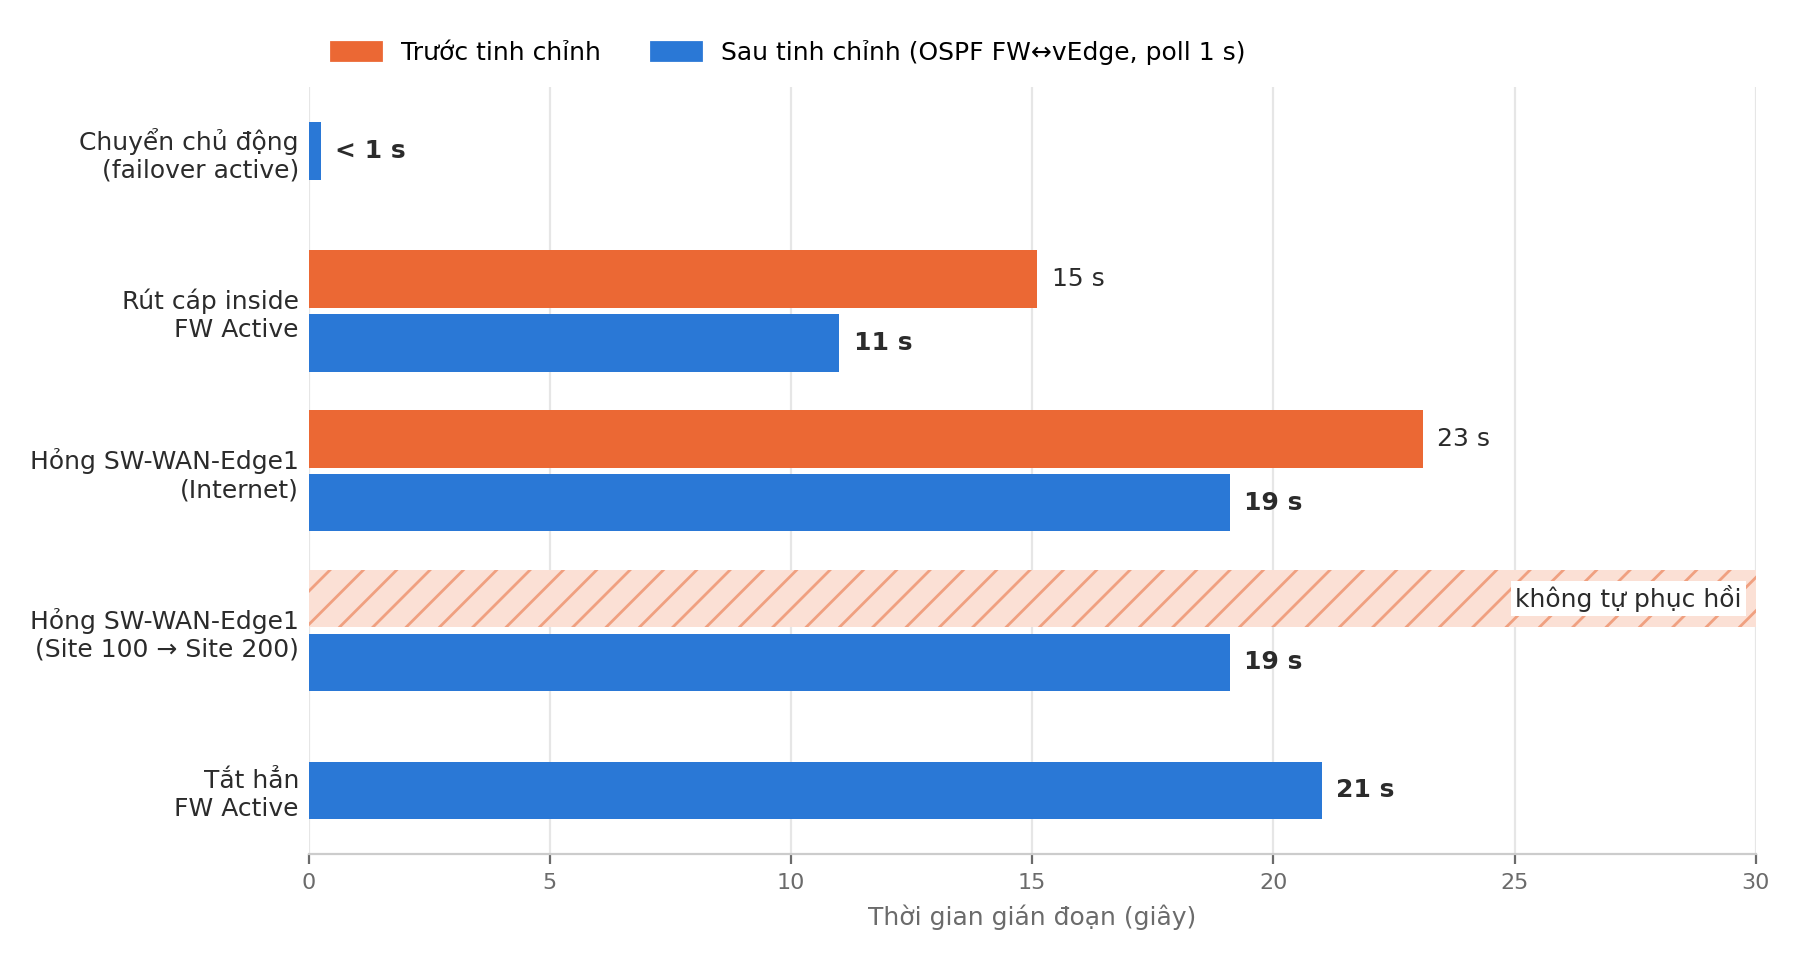
\includegraphics[width=0.9\textwidth]{image/fw-ha-failover.png}
    \caption{Thời gian gián đoạn khi gây lỗi cặp tường lửa HA Site 100, trước và sau tinh chỉnh}
    \label{fig:fw_ha_failover}
\end{figure}

Trong quá trình triển khai có ba vấn đề đáng chú ý. Thứ nhất, cách đấu dây ban đầu nối đơn vị Standby vào các mạng \texttt{/30} khác với đơn vị Active, nên khi chuyển vai trò, các thiết bị xung quanh không còn cùng mạng với tường lửa mới: failover thực chất chưa từng hoạt động. Việc chuyển sang các mạng transit chung \texttt{/29} qua VLAN 101--104 đã khắc phục điều này. Thứ hai, khi cây dữ liệu của SDN Controller chặn đường lên Core-SW2, Core-SW2 không nghe được VRRP của Core-SW1 và cùng lên Master (split-brain); thêm VLAN 10--40 vào Po10 đã đưa Core-SW2 về Backup ở cả năm VLAN. Thứ ba, trong hai ngày 01--02/11/2026 cả hai đơn vị ASAv khởi động lại lặp do lỗi phần mềm (\texttt{show crashinfo} ghi lỗi trong tiến trình cập nhật bảng định tuyến) khi dùng tuyến mặc định có \texttt{track} theo \texttt{sla monitor}; bỏ \texttt{track} và \texttt{sla monitor} trên tường lửa biên, để OSPF với vEdge đảm nhận phát hiện lỗi, đã làm tường lửa chạy ổn định trở lại.

\subsection{Triển khai SDN tại Campus chính}

\subsubsection{Cấu hình Open vSwitch và Controller}

Mỗi OVS được thiết lập bằng các lệnh \texttt{ovs-vsctl} trong một dịch vụ khởi động chạy mỗi lần boot (Khối lệnh~\ref{lst:ovs_controller_ch4}, ví dụ Access-SW1).

\begin{lstlisting}[style=customcode,caption={Thiết lập bridge OpenFlow trên Access-SW1},label={lst:ovs_controller_ch4}]
ovs-vsctl set bridge br0 protocols=OpenFlow13
ovs-vsctl set bridge br0 other_config:datapath-id=0000000000000044
ovs-vsctl set bridge br0 fail_mode=secure
ovs-vsctl set bridge br0 stp_enable=false
ovs-vsctl set bridge br0 other_config:disable-in-band=true
ovs-vsctl set port ens4 trunks=10,20,30,40,90,99
ovs-vsctl set port ens6 tag=10
ovs-vsctl set-controller br0 tcp:10.1.99.10:6653 tcp:10.1.99.10:6654
\end{lstlisting}

Trên Controller, Ryu được chạy dưới dạng dịch vụ systemd (ưu tiên CPU cao), nạp đồng thời ba ứng dụng \texttt{campus\_switch\_13.py}, \texttt{campus\_noc\_monitor.py} và \texttt{ryu.app.ofctl\_rest}, lắng nghe OpenFlow tại TCP 6653 và phục vụ Campus SDN Console tại TCP 8080 (Hình~\ref{fig:console_tongquan}, Hình~\ref{fig:console_topology}). Địa chỉ Controller thứ hai (TCP 6654) được dành cho Controller dự phòng; khi không có tiến trình lắng nghe, OVS chỉ thử kết nối lại định kỳ, không ảnh hưởng chuyển tiếp. Ứng dụng có bộ kiểm thử đơn vị mô phỏng cây dữ liệu và kênh quản trị trước mỗi lần triển khai. Phân vùng \texttt{/boot} của sáu OVS và Controller được đánh dấu \texttt{nofail} để máy ảo không dừng ở chế độ khẩn cấp khi khởi động đồng loạt chậm.

\begin{figure}[H]
    \centering
    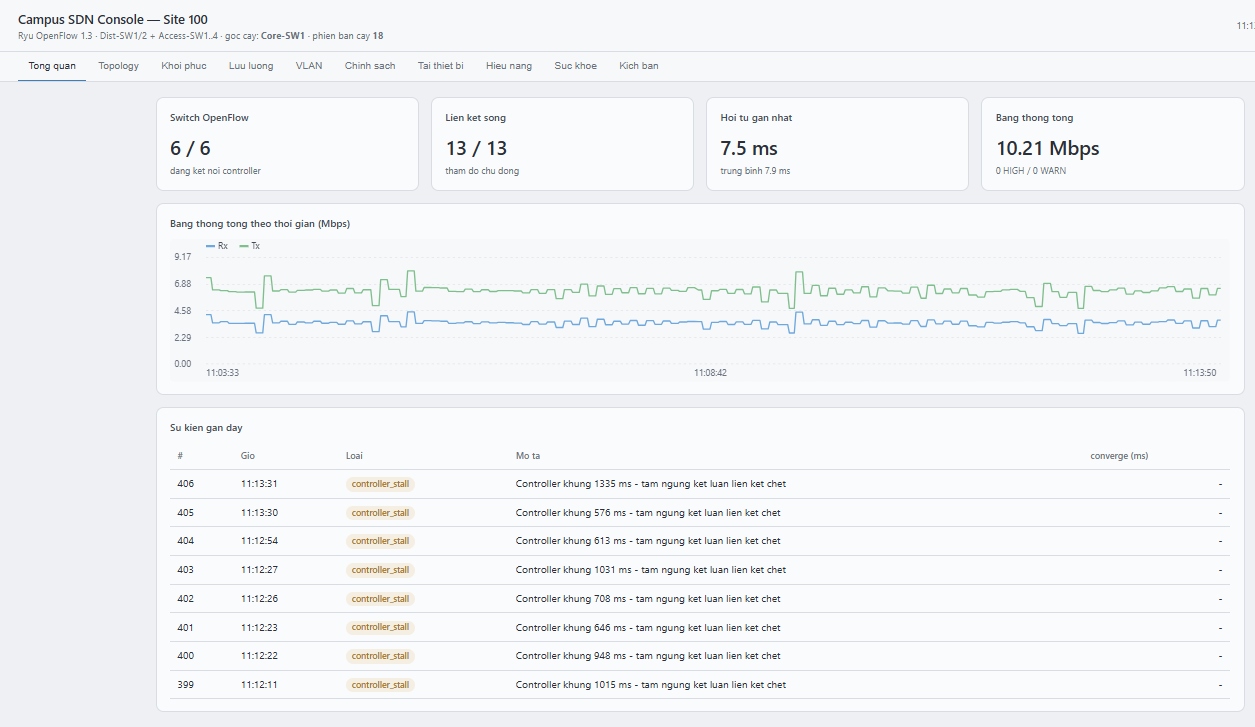
\includegraphics[width=\textwidth]{image/sdn-console-tongquan.png}
    \caption{Campus SDN Console -- trang Tổng quan: 6/6 switch, 13/13 liên kết, thời gian hội tụ và nhật ký sự kiện}
    \label{fig:console_tongquan}
\end{figure}

\begin{figure}[H]
    \centering
    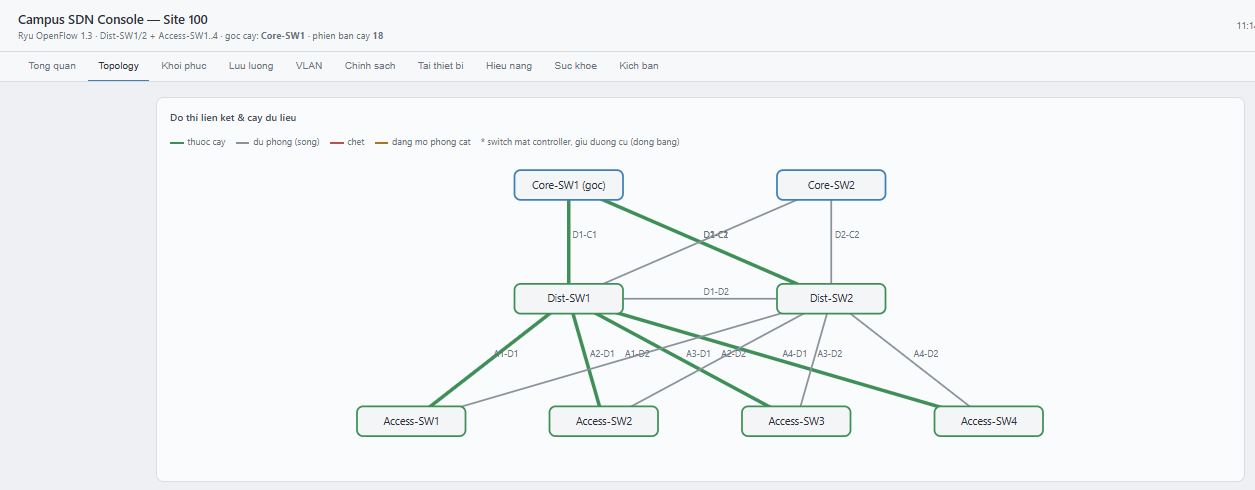
\includegraphics[width=\textwidth]{image/sdn-console-topology.png}
    \caption{Campus SDN Console -- đồ thị liên kết và cây dữ liệu khi mạng bình thường: gốc Core-SW1, bốn Access đi lên Dist-SW1 (xanh: thuộc cây, xám: dự phòng)}
    \label{fig:console_topology}
\end{figure}

\subsubsection{Các chức năng của Campus SDN Console}\label{sec:sdn_console}

Campus SDN Console là giao diện web do nhóm tự phát triển, chạy ngay trong tiến trình Ryu (ứng dụng \texttt{campus\_noc\_monitor.py}), không dùng thư viện ngoài vì VLAN 99 không ra Internet. Mọi thao tác trên giao diện đều gọi REST API của chính Controller, nên cũng có thể tự động hóa bằng script. Bảng~\ref{tab:sdn_console_tabs} tóm tắt mười trang chức năng và mục tiêu đánh giá tương ứng; các hình tiếp theo được chụp trực tiếp trên hệ thống đang vận hành.

\begin{table}[H]
    \centering
    \small
    \caption{Các trang chức năng của Campus SDN Console}
    \label{tab:sdn_console_tabs}
    \begin{tabularx}{\textwidth}{|P{2.4cm}|Y|}
        \hline
        \textbf{Trang} & \textbf{Chức năng} \\
        \hline
        Tổng quan & Số switch OpenFlow và liên kết đang sống, thời gian hội tụ gần nhất và trung bình, băng thông tổng theo thời gian, nhật ký sự kiện \\
        \hline
        Topology & Đồ thị liên kết và cây dữ liệu; cắt/khôi phục từng liên kết ở chế độ mô phỏng đứt ngầm (\textit{silent}) hoặc tắt cổng (\textit{admin}) \\
        \hline
        Khôi phục & Ping liên tục từ Controller tới máy trạm (chu kỳ 0,1--1 giây), biểu đồ RTT và vùng mất gói, bảng sự kiện với thời gian phát hiện, hội tụ, tổng; xuất CSV \\
        \hline
        Lưu lượng & Mbit/s theo từng switch và từng cổng (pps, drop, phần trăm sử dụng) \\
        \hline
        VLAN & Thêm/xóa VLAN, gán cổng access bằng một lệnh API cho toàn bộ OVS; sinh sẵn đoạn cấu hình IOS cho Core-SW1/2; so sánh thời gian với cách cấu hình truyền thống \\
        \hline
        Chính sách & Thêm luật chặn/cho phép theo VLAN, dải địa chỉ, giao thức, cổng, hai chiều, độ ưu tiên; bật/tắt/xóa; bộ đếm gói khớp từng luật \\
        \hline
        Tải thiết bị & Mbit/s, pps, drop, packet-in/s, số flow và lookup/s của từng OVS; lưu lượng uplink và CPU của Core qua SNMP; CPU/RAM của Controller \\
        \hline
        Hiệu năng & Ma trận RTT giữa các VLAN (trong VLAN qua OVS, khác VLAN qua Core) và chi tiết từng cặp máy trạm \\
        \hline
        Sức khỏe & Kênh điều khiển của từng switch, cha trong cây, các đường quản trị VLAN 99 đang dùng, số lần nối lại; số lần Controller khựng; vai trò STP của VLAN 99 trên Core-SW1 qua SNMP; cảnh báo tự sinh \\
        \hline
        Kịch bản & Chạy tự động sáu kịch bản cắt liên kết S1--S6 và kết luận Đạt/Không đạt theo ngưỡng gián đoạn \\
        \hline
    \end{tabularx}
\end{table}

Hình~\ref{fig:console_topology_s1} chụp đúng lúc kịch bản S1 đang cắt liên kết Dist-SW1--Core-SW1 (nét đứt màu cam): Controller đã tính lại cây, mọi Access đi lên Core-SW1 qua Dist-SW2, liên kết D1-C1 ở trạng thái \textit{cắt (silent)}, mười hai liên kết còn lại vẫn sống.

\begin{figure}[H]
    \centering
    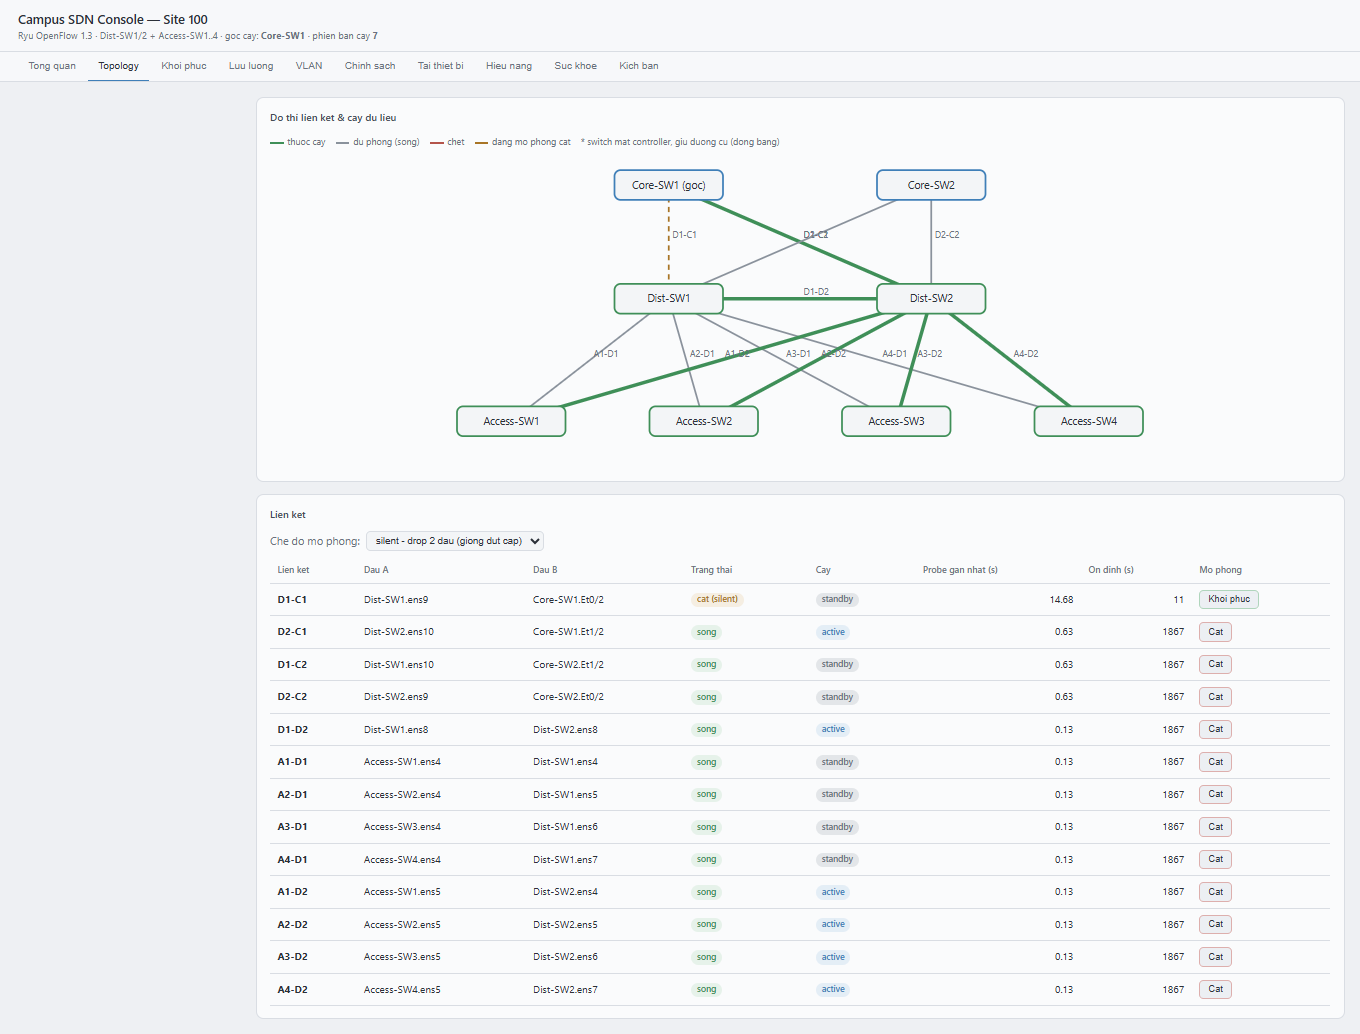
\includegraphics[width=\textwidth]{image/sdn-console-topology-s1-20261108.png}
    \caption{Trang Topology trong lúc kịch bản S1 cắt liên kết D1-C1: cây dữ liệu chuyển sang đi qua Dist-SW2}
    \label{fig:console_topology_s1}
\end{figure}

Trang VLAN (Hình~\ref{fig:console_vlan}) liệt kê năm VLAN đang quản lý cùng các cổng access trên bốn Access và cho phép thêm VLAN mới chỉ bằng một biểu mẫu. Vì Core-SW1/2 là switch truyền thống nằm ngoài OpenFlow, Controller sinh sẵn đoạn lệnh IOS (VLAN, SVI, VRRP, \texttt{ip helper-address}) để áp lên hai Core.

\begin{figure}[H]
    \centering
    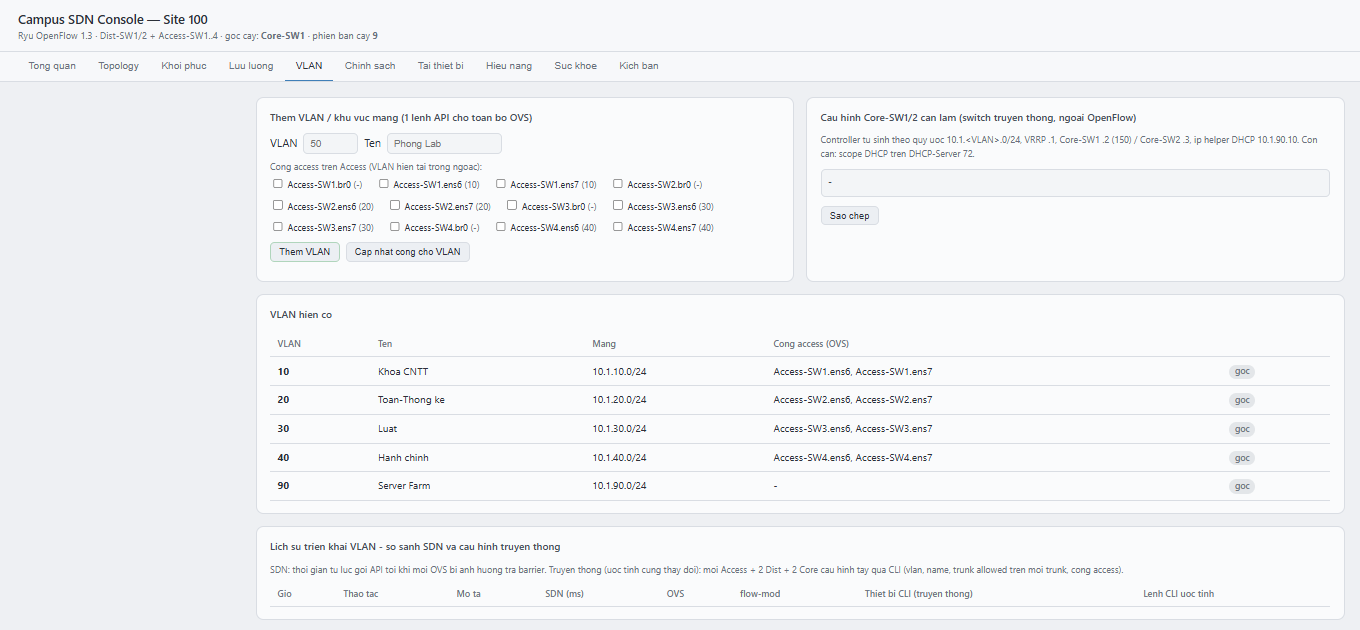
\includegraphics[width=\textwidth]{image/sdn-console-vlan-20261108.png}
    \caption{Trang VLAN: năm VLAN và cổng access trên các OVS}
    \label{fig:console_vlan}
\end{figure}

Trang Chính sách (Hình~\ref{fig:console_policy}) được kiểm thử với luật chặn ICMP hai chiều giữa VLAN 10 và VLAN 40: luật được cài lên bốn Access trong \textbf{12,6 ms} (12 flow-mod); năm gói ping từ PC-CNTT-S100-1 (VLAN 10) tới máy VLAN 40 đều bị chặn và bộ đếm của luật tăng đúng 5 gói, trong khi ping cùng máy đó tới VLAN 20 vẫn thông (3/3). Sau khi xóa luật, ping VLAN 10 -- VLAN 40 thông trở lại.

\begin{figure}[H]
    \centering
    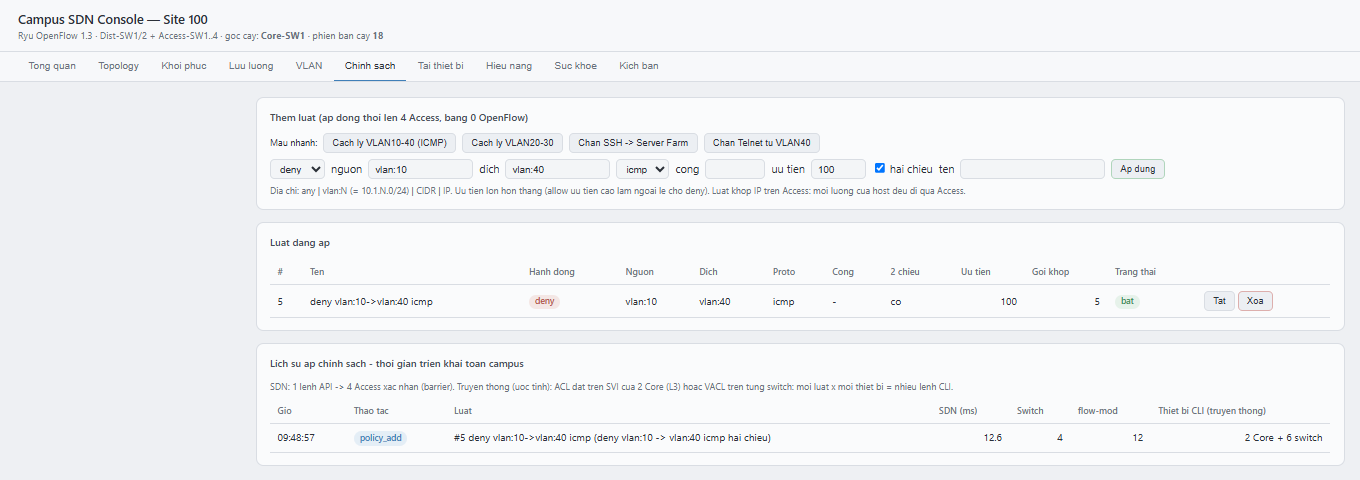
\includegraphics[width=\textwidth]{image/sdn-console-chinhsach-20261108.png}
    \caption{Trang Chính sách: luật chặn ICMP VLAN 10 -- VLAN 40 khớp 5 gói, thời gian áp toàn campus 12,6 ms}
    \label{fig:console_policy}
\end{figure}

Trang Tải thiết bị (Hình~\ref{fig:console_load}) cho thấy tải điều khiển của mỗi switch chỉ khoảng 17--29 packet-in/s, không có drop, Ryu dùng khoảng 4--9\% CPU; số flow trên mỗi Access chỉ 6 (bảng 0) và 3 (bảng 1) vì luồng đã học được chuyển thẳng bằng flow.

\begin{figure}[H]
    \centering
    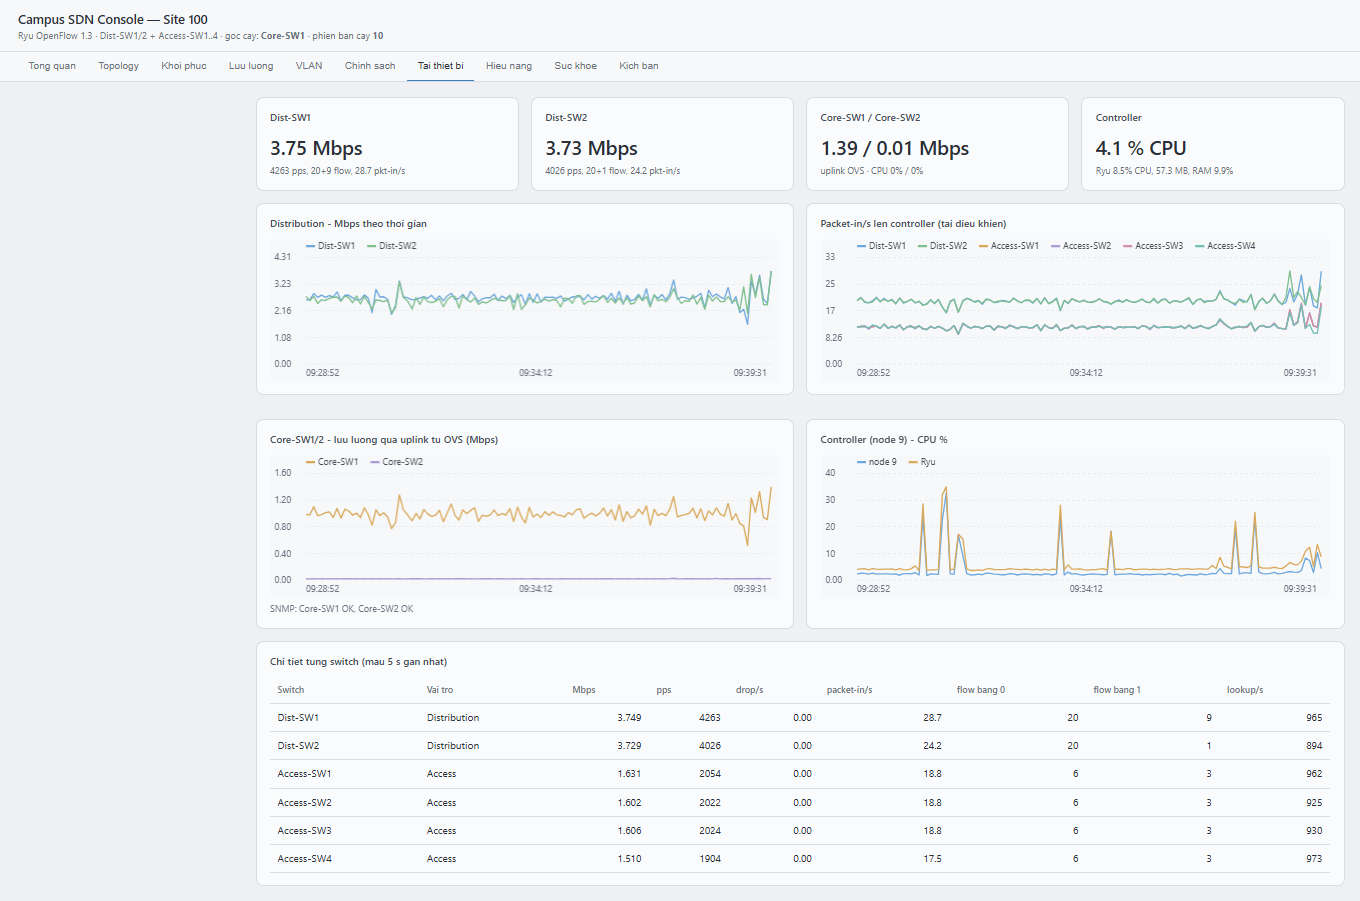
\includegraphics[width=\textwidth]{image/sdn-console-taithietbi-20261108.png}
    \caption{Trang Tải thiết bị: lưu lượng Distribution, packet-in/s, uplink Core qua SNMP và CPU Controller}
    \label{fig:console_load}
\end{figure}

Trang Sức khỏe (Hình~\ref{fig:console_health}) giám sát chính mặt phẳng điều khiển: sáu switch đều kết nối, mỗi Distribution có hai đường quản trị VLAN 99 và mỗi Access có bốn đường đồng thời; hai cổng Et0/2, Et1/2 của Core-SW1 đều ở vai trò \textit{designated} (đúng trạng thái mong đợi, không có vòng VLAN 99). Trang này cũng ghi nhận Controller bị khựng nhiều lần (69 lần trong một giờ, lâu nhất 4,2 giây, phần lớn ngay sau khi khởi động đồng loạt) --- đây là hạn chế về tài nguyên đã nêu ở Mục~\ref{sec:bai_hoc_sdn}; cơ chế ân hạn giữ cho các lần khựng này không bị coi là liên kết chết.

\begin{figure}[H]
    \centering
    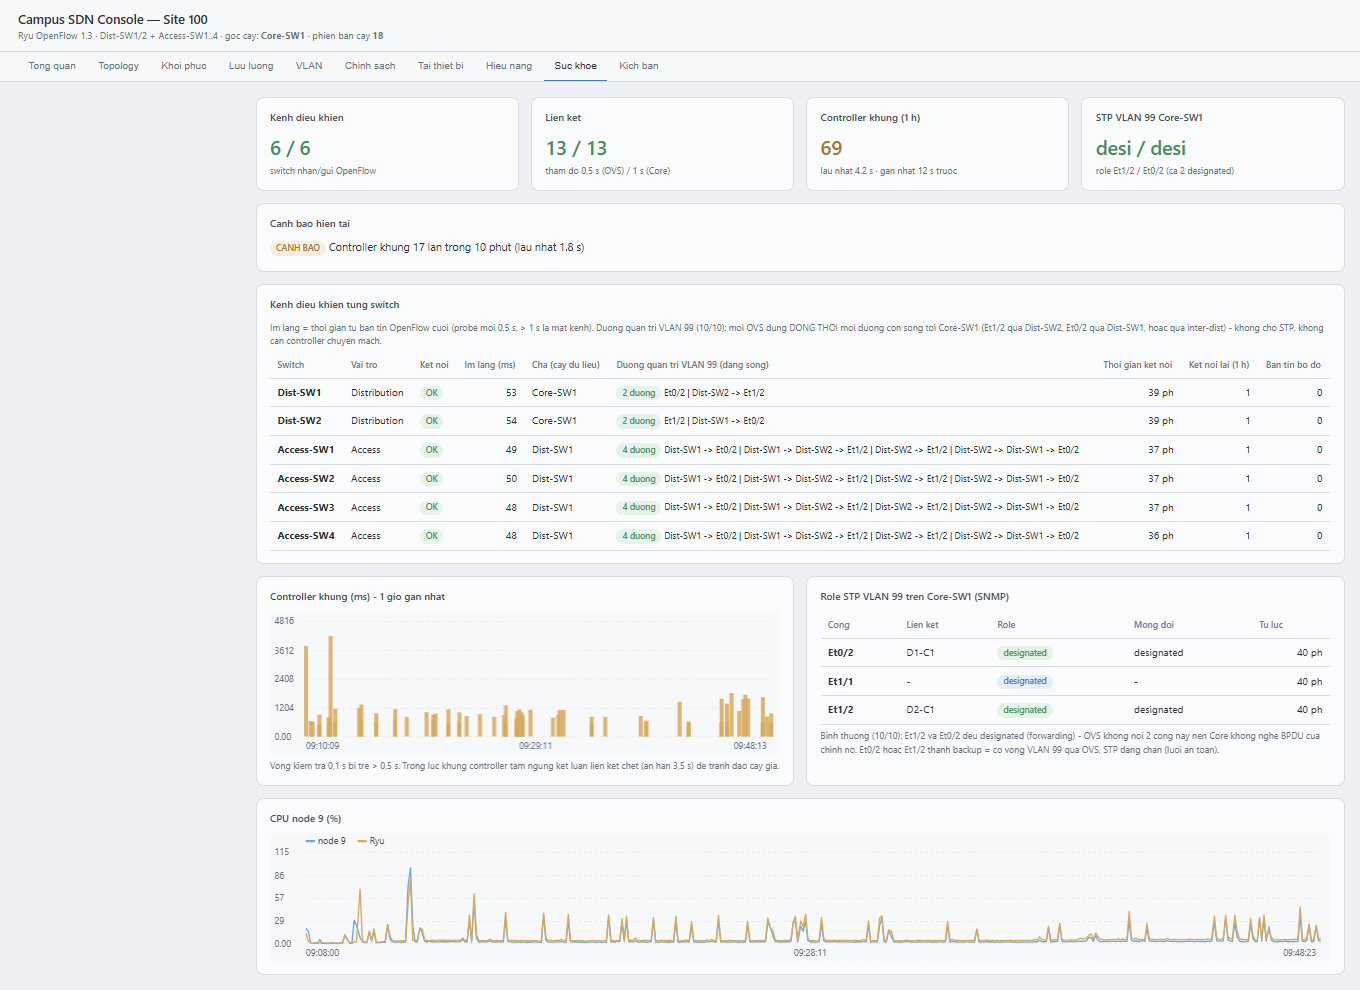
\includegraphics[width=\textwidth]{image/sdn-console-suckhoe-20261108.png}
    \caption{Trang Sức khỏe: kênh điều khiển từng switch, đường quản trị VLAN 99 nhiều đường và vai trò STP trên Core-SW1}
    \label{fig:console_health}
\end{figure}

\subsubsection{Các vấn đề kỹ thuật và nguyên nhân gốc}\label{sec:bai_hoc_sdn}

Phần SDN là phần tốn nhiều công sức nhất vì toàn bộ hành vi mà switch truyền thống có sẵn (học MAC, chống vòng, dự phòng) phải được Controller hiện thực lại, trong khi kênh điều khiển lại đi chung hạ tầng với dữ liệu. Các vấn đề chính được tổng hợp trong Bảng~\ref{tab:loi_sdn}.

\begingroup
\small
\begin{longtable}{|L{3.0cm}|L{5.2cm}|L{5.3cm}|}
    \caption{Các vấn đề SDN, nguyên nhân gốc và cách khắc phục}\label{tab:loi_sdn} \\
    \hline
    \textbf{Hiện tượng} & \textbf{Nguyên nhân gốc} & \textbf{Khắc phục} \\
    \hline
    \endfirsthead
    \hline
    \textbf{Hiện tượng} & \textbf{Nguyên nhân gốc} & \textbf{Khắc phục} \\
    \hline
    \endhead
    \hline
    \endfoot
    Máy trạm không nhận DHCP; gói bị flood với VLAN 0 & Khi switch mất kết nối tạm thời, bộ xử lý sự kiện xóa luôn bảng cổng access; khi kết nối lại, VLAN của cổng không còn nên được xác định là 0 & Giữ cấu hình cổng tĩnh khi switch mất kết nối; bổ sung hàm tra VLAN từ bảng cấu hình \\
    \hline
    Frame có thẻ VLAN nhưng Controller không nhận ra VLAN & Trường match của Packet-In chỉ có \texttt{in\_port}, thẻ 802.1Q nằm trong dữ liệu gói & Controller tự phân tích thẻ trong dữ liệu; tạo hành động gắn/bóc thẻ theo từng cổng ra \\
    \hline
    DHCP chỉ có Discover, Offer, thiếu Request/ACK & Cài flow unicast dùng trường \texttt{dl\_vlan} của OpenFlow 1.0, gây ngoại lệ làm dừng bộ xử lý & Dùng \texttt{vlan\_vid = OFPVID\_PRESENT | vlan} theo OpenFlow 1.3 \\
    \hline
    Bão broadcast VLAN 99 (130.000--250.000 gói/s), OVS liên tục mất kết nối Controller & VLAN 99 được flood trên toàn bộ lưới (Access nối kép, inter-dist, bốn đường lên Core) trong khi flow khởi động dùng hành động \texttt{NORMAL} & Thay flow \texttt{NORMAL} bằng flow tường minh; tính đường quản trị riêng cho VLAN 99 \\
    \hline
    Mỗi khi một OVS khởi động lại, bão ARP khoảng 200.000 gói/s lan ra toàn mạng & Chế độ in-band của OVS tự cài các flow ẩn (không hiển thị khi liệt kê flow) có hành động \texttt{NORMAL} cho ARP khi switch chưa kết nối Controller; nhật ký OVS có cảnh báo \texttt{in\_band: cannot find route for controller} & Tắt in-band (\texttt{disable-in-band=true}) vì kênh điều khiển đã đi qua bridge quản trị riêng \\
    \hline
    Sau khi cây đổi, dữ liệu vẫn mất thêm 11--12 giây & Core-SW1/2 (switch truyền thống) vẫn giữ vị trí MAC cũ của máy trạm & Controller phát RARP thay máy trạm theo đường mới ngay sau khi cài cây \\
    \hline
    Đứt liên kết Dist-SW2 -- Core-SW1 làm sáu OVS mất Controller tới 10 giây khi khôi phục & Khung VLAN 99 đi vòng Core-SW1 $\rightarrow$ OVS $\rightarrow$ Core-SW1 nên Core nghe chính BPDU của mình; khi khôi phục, cổng E1/2 rơi vào trạng thái \textit{Dispute} của RSTP và phải chờ hai lần forward-delay & Thiết kế lại kênh VLAN 99 không phụ thuộc STP: khung từ cổng Core không bao giờ ra cổng Core khác; mỗi switch có nhiều đường quản trị đồng thời; chống phản xạ theo MAC nguồn \\
    \hline
    Cho Core-SW2 tham gia VLAN 99 gây bão khoảng 40.000 gói/s & OVS flood tĩnh trong VLAN 99, hai router cùng VLAN định tuyến ngược unicast của nhau & Core-SW2 không tham gia VLAN 99 (SVI tắt, tuyến tĩnh qua Po10) \\
    \hline
    Tắt hẳn Dist-SW2 làm bốn VLAN mất 100\% khoảng 3,5 phút & Controller loại các Access mất kết nối khỏi cây và chặn cổng Dist-SW1 nối xuống chúng, dù các Access vẫn chạy bằng flow cũ & ``Đóng băng'' Access mất kết nối làm lá trên liên kết cha cũ; thêm đường quản trị dự phòng qua Dist-SW1 \\
    \hline
    Sau một lần cắt kép, Dist-SW2 mất Controller vĩnh viễn & Flow bảo vệ VLAN 99 bị xóa trước rồi mới cài lại; kết nối đứt giữa chừng nên bản cài mới không tới switch & Chỉ ghi đè flow quản trị, không xóa trước \\
    \hline
    Controller khựng 0,5--9 giây theo cụm, có lúc cả sáu OVS mất kết nối & ONOS chạy song song chiếm hơn một vCPU của máy Controller (2 vCPU); Ryu bị đói CPU & Tắt ONOS, ưu tiên CPU cho Ryu; thêm ân hạn để khựng không bị coi là liên kết chết \\
    \hline
    Vòng thăm dò đứng hẳn khi một switch chết & Ryu 4.34 chờ vô hạn khi hàng đợi gửi của kết nối chết đầy & Giới hạn thời gian chờ gửi 0,5 giây; Echo 2 giây $\times$ 3 lần \\
    \hline
    Khởi động đồng loạt: một Access vào chế độ khẩn cấp & Máy ảo bị chậm CPU lúc boot, gắn \texttt{/boot} quá thời gian & Đánh dấu \texttt{nofail} cho \texttt{/boot} trên sáu OVS và Controller \\
\end{longtable}
\endgroup

Bài học rút ra là trong mạng SDN in-band, mặt phẳng điều khiển phải được thiết kế như một mạng riêng (không vòng, nhiều đường, khởi động độc lập với Controller) trước khi xây dựng logic cho mặt phẳng dữ liệu; Controller phải phân biệt ``mất kênh điều khiển'' với ``liên kết dữ liệu chết''; và mọi kết luận về nguyên nhân phải dựa trên bắt gói, trạng thái STP hoặc thống kê CPU theo từng thời điểm thay vì suy đoán.

\subsubsection{Kết quả kiểm thử SDN}

\textbf{Chức năng cơ bản:} sau khi khởi động đồng thời toàn bộ Campus chính, sáu switch kết nối OpenFlow 1.3 đầy đủ, 13/13 liên kết sống. Tám máy trạm xin địa chỉ DHCP thành công với đủ bốn bản tin DORA, nhận đúng scope, gateway \texttt{.1}, DNS \texttt{10.1.90.10} và tên miền \texttt{campus.internal} (VLAN 10: \texttt{.100}, \texttt{.101}; VLAN 20: \texttt{.100}, \texttt{.101}; VLAN 30: \texttt{.100}, \texttt{.101}; VLAN 40: \texttt{.100}; máy Ubuntu PC-HanhChinh-S100: \texttt{10.1.40.102}); ping gateway, DHCP Server và liên VLAN đều thành công. Khi khởi động lại Controller, sáu switch kết nối lại sau khoảng 15 giây; khởi động lại từng Access không phát sinh bão broadcast (lưu lượng lớn nhất khoảng 365 gói/s so với 200.000 gói/s trước khi khắc phục).

\textbf{Đánh giá theo năm tiêu chí định lượng} (Bảng~\ref{tab:sdn_muc_tieu}): các phép đo được thực hiện bằng script tự động, ping 0,1 giây từ Controller tới máy trạm.

\begin{table}[H]
    \centering
    \small
    \caption{Kết quả đánh giá SDN theo năm tiêu chí}
    \label{tab:sdn_muc_tieu}
    \begin{tabularx}{\textwidth}{|P{3.3cm}|Y|}
        \hline
        \textbf{Tiêu chí} & \textbf{Kết quả đo} \\
        \hline
        Thời gian thêm VLAN & SDN: \textbf{3,8 ms} (một lệnh API, đến khi switch xác nhận); cùng thay đổi trên mỗi Core IOL cần 18 lệnh CLI, script đẩy xong khoảng 1,2 giây/thiết bị khi chờ đúng prompt. Đo đầu cuối (3 lần, sai số khoảng 5 giây, máy trạm đặt IP tĩnh): xong SDN và hai Core sau \textbf{5,3 giây}, ping được gateway sau 37,8 giây, DHCP Server sau 42,0 giây. Chưa gồm bước tạo scope DHCP làm tay \\
        \hline
        Thời gian khôi phục khi mất liên kết & Hội tụ của Controller dưới 16 ms; gián đoạn dữ liệu chủ yếu là thời gian phát hiện: cổng báo down 0--0,3 giây, đứt ngầm Access--Distribution 1,8 giây, Distribution--Core 2,9--3,4 giây, mất hẳn Dist-SW1 1,9 giây; khi liên kết trở lại 0--0,4 giây \\
        \hline
        Hiệu năng giữa các VLAN & RTT nền (nhỏ nhất) \textbf{0,38 ms} trong VLAN (lớp 2 qua OVS) và \textbf{1,3 ms} khác VLAN (qua Core). Khi 69/74 node chạy đồng thời và máy chủ ổn định (49 cặp, 10 gói/cặp): RTT trung bình 0,43 ms và 1,57 ms, lớn nhất 13,2 ms, jitter dưới 0,4 ms, mất gói 0\% (490/490). Thông lượng TCP đo bằng iperf3: khoảng 1,2 Gbit/s trong cùng Access, 170 Mbit/s liên VLAN (Bảng~\ref{tab:sdn_tai_cao}). Khi máy chủ quá tải, cùng phép đo từng cho RTT 7--16 ms và mất 2,6--6,9\% \\
        \hline
        Tải Core/Distribution & Lúc rảnh khoảng 85 packet-in/s, Ryu khoảng 4\% CPU; không tăng theo lưu lượng người dùng (luồng đã học đi thẳng bằng flow). Khi tăng lên 1000 MAC mới/giây (1088 packet-in/s), Ryu tăng tuyến tính tới 41,3\% CPU, luồng đang chạy không mất gói (100/100), 6/6 switch giữ kết nối (Hình~\ref{fig:bd_packetin}). Dưới tải dữ liệu, CPU tiến trình Dist-SW1 và Access-SW1 lên tối đa 84\% và 79\% (Bảng~\ref{tab:cpu_ram}) \\
        \hline
        Áp chính sách tập trung & Luật chặn ICMP giữa VLAN 10 và VLAN 40 áp lên bốn Access trong \textbf{8,0--12,6 ms} (12 flow-mod), gỡ trong 5,2--10,8 ms; bộ đếm của luật khớp đúng số gói bị chặn (5/5); luồng khác không bị ảnh hưởng (Hình~\ref{fig:console_policy}) \\
        \hline
    \end{tabularx}
\end{table}

\textbf{Kịch bản tự phục hồi:} trang Kịch bản của Console chạy tự động sáu kịch bản cắt liên kết (mô phỏng đứt ngầm, giữ 15 giây) với tiêu chí đạt: gián đoạn khi cắt không quá 5 giây, khi khôi phục không quá 3 giây và mạng trở về đủ 13/13 liên kết, 6/6 switch. Bảng~\ref{tab:sdn_kich_ban} là kết quả trên hệ thống hoàn chỉnh (ping 0,1 giây tới một máy trạm mỗi VLAN 10--40), cột cuối ghi kết quả trước khi tắt ONOS và thiết kế lại kênh VLAN 99 để so sánh.

\begin{table}[H]
    \centering
    \small
    \caption{Kết quả kịch bản tự phục hồi SDN (ping 0,1 giây tới bốn VLAN)}
    \label{tab:sdn_kich_ban}
    \begin{tabularx}{\textwidth}{|P{3.0cm}|P{1.9cm}|P{1.9cm}|P{1.6cm}|Z|}
        \hline
        \textbf{Kịch bản} & \textbf{Gián đoạn khi cắt} & \textbf{Khi khôi phục} & \textbf{Về đủ sau} & \textbf{Trước khi sửa} \\
        \hline
        S1: D1-C1 & 3,2 s & 0 & 2,0 s & Đạt \\
        \hline
        S2: A4-D1 & 2,0 s (VLAN 40) & 0 & 1,5 s & Đạt \\
        \hline
        S3: D1-D2 & 0 & 0 & 2,0 s & Đạt (Dist-SW1 mất Controller khoảng 1 s) \\
        \hline
        S4: D2-C1 & 0 & 0 & 1,5 s & Không đạt (10,9 s khi khôi phục) \\
        \hline
        S5: A4-D1 + D2-C1 & 3,5 s (VLAN 40) & 0,1 s & 2,5 s & Không đạt (15 s khi cắt, 10,3 s khi khôi phục) \\
        \hline
        S6: D1-C1 + D1-C2 & 3,6 s & 0 & 1,5 s & Đạt \\
        \hline
    \end{tabularx}
\end{table}

\begin{figure}[H]
    \centering
    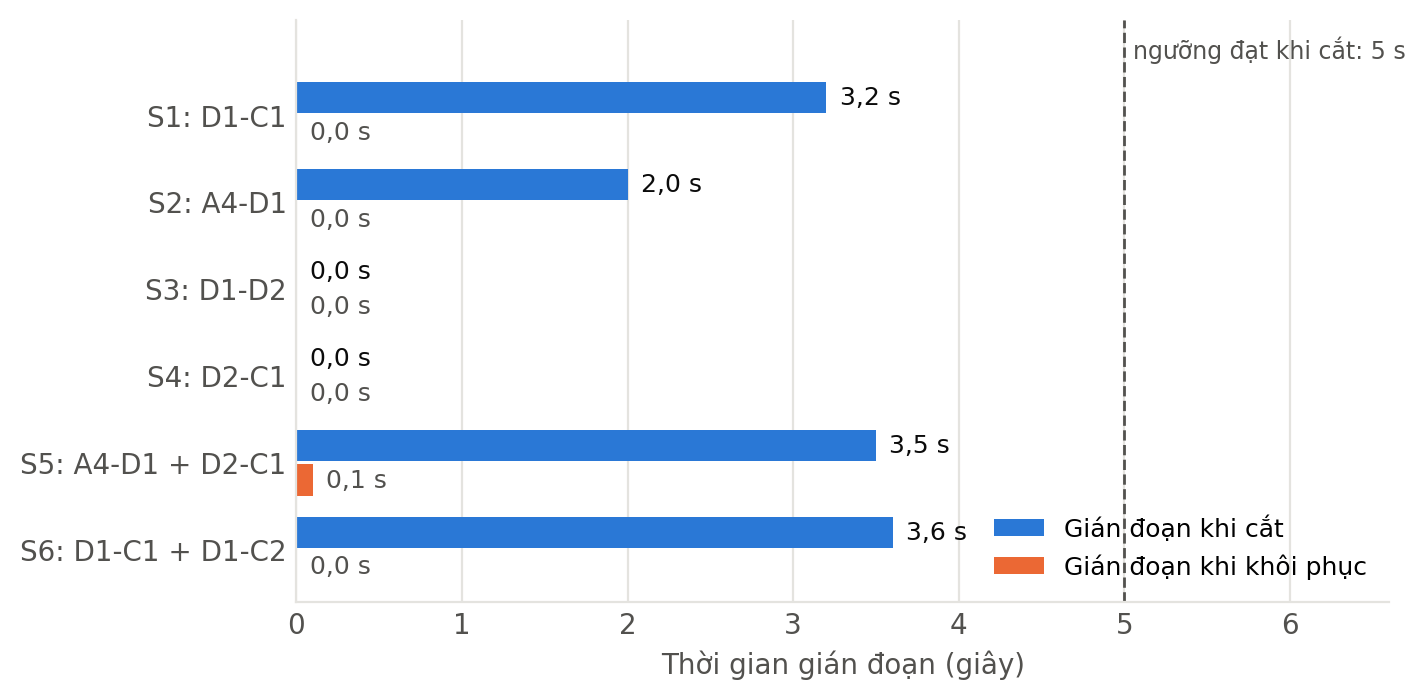
\includegraphics[width=0.95\textwidth]{image/bd-sdn-kichban.png}
    \caption{Gián đoạn của sáu kịch bản tự phục hồi SDN so với ngưỡng đạt 5 giây}
    \label{fig:bd_sdn}
\end{figure}

Trên hệ thống hoàn chỉnh, \textbf{cả sáu kịch bản đều đạt} (Hình~\ref{fig:bd_sdn}), không switch nào mất Controller trong cả loạt thử và mạng luôn trở về đủ 13/13 liên kết, 6/6 switch sau 1,5--2,5 giây (Hình~\ref{fig:console_kichban}). Phép cắt \textbf{thật} (hạ giao diện ảo trên máy chủ EVE-NG, tương đương rút dây, giữ 20 giây) cho kết quả tương tự: D2-C1 không mất gói; A4-D1 kèm D2-C1 làm VLAN 40 mất 3,2 giây, khôi phục 0,2 giây; D1-C1 mất 2,8--3,1 giây, khôi phục không quá 0,4 giây. Khi tắt hẳn Dist-SW2, dữ liệu chỉ mất 0--5 gói và bốn Access nối lại Controller qua Dist-SW1 sau khoảng 11 giây; khi bật lại không mất gói.

Hình~\ref{fig:bd_vlan} tách thời gian thêm VLAN đầu--cuối theo từng mốc: phần cấu hình chỉ mất khoảng 5 giây, phần lớn thời gian còn lại là chờ máy trạm dùng được VLAN mới.

\begin{figure}[H]
    \centering
    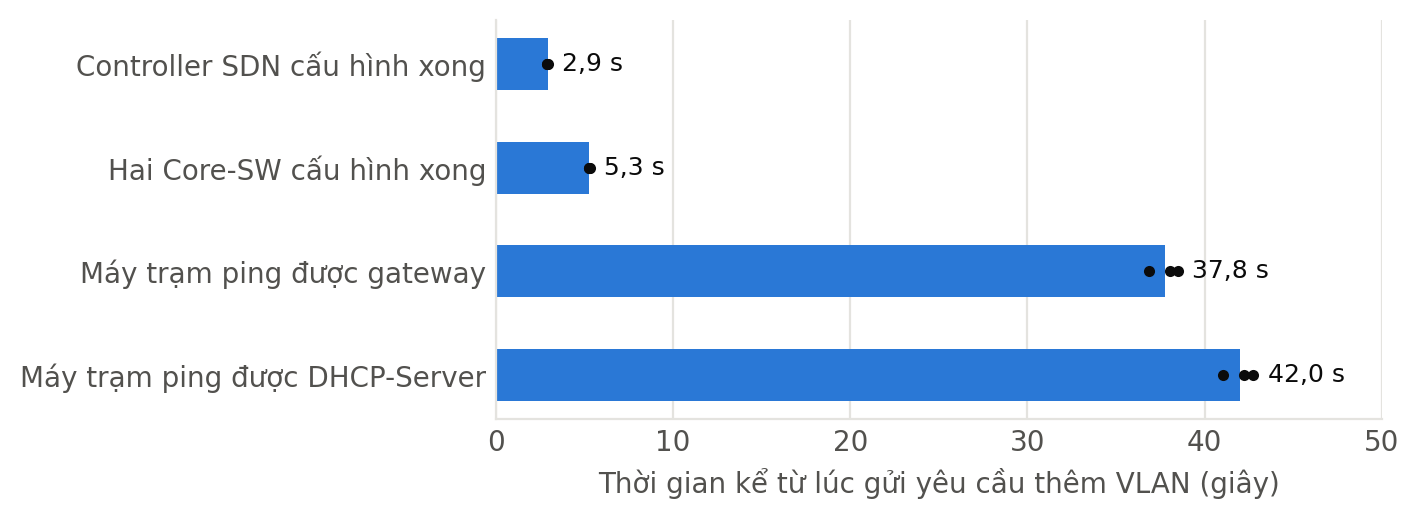
\includegraphics[width=0.9\textwidth]{image/bd-vlan-daucuoi.png}
    \caption{Thời gian thêm VLAN đầu--cuối theo từng mốc (3 lần đo; cột là trung bình, chấm là từng lần)}
    \label{fig:bd_vlan}
\end{figure}

Hình~\ref{fig:console_khoiphuc} là trang Khôi phục: bốn luồng ping liên tục và bảng sự kiện ghi thời gian phát hiện (khoảng 2--3,6 giây, chủ yếu là thời gian chờ thăm dò liên kết hết hạn) và thời gian Controller hội tụ (5--12 ms) cho từng lần cắt.

\begin{figure}[H]
    \centering
    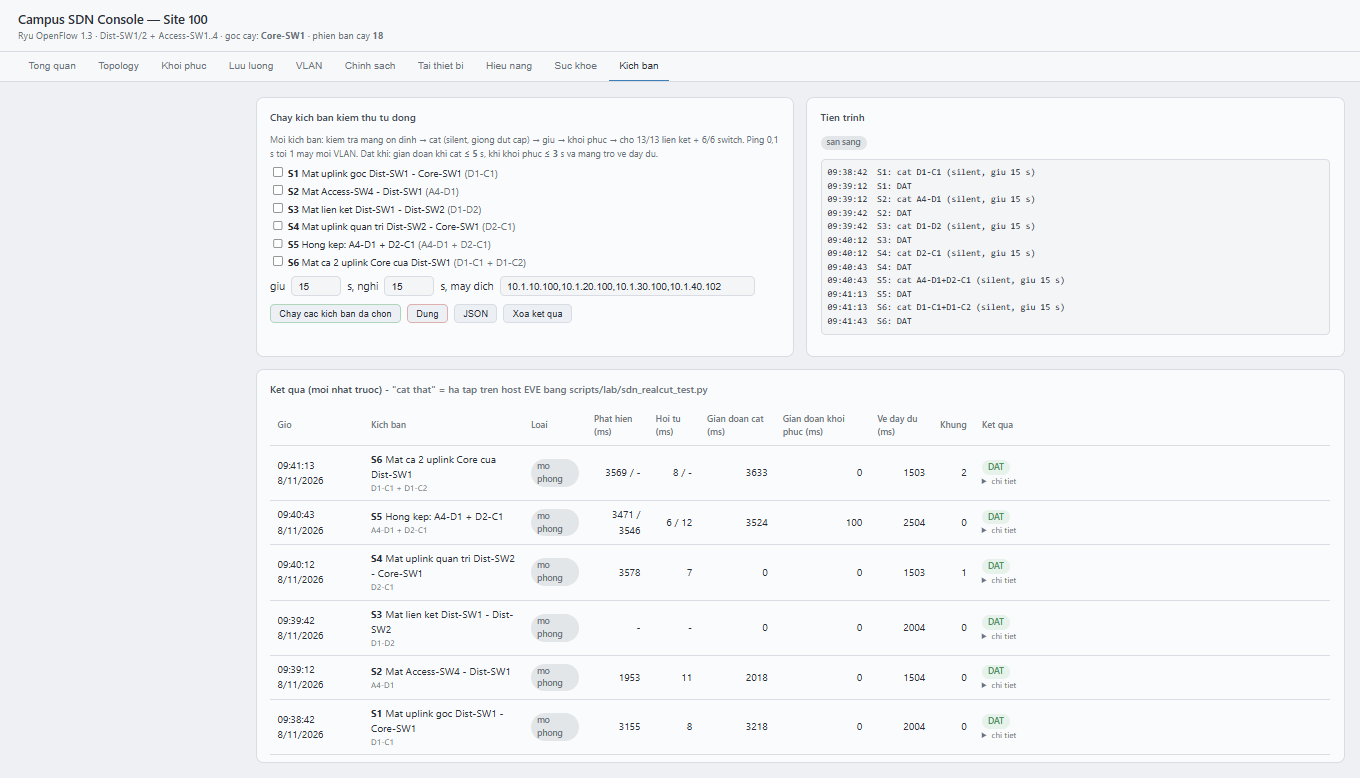
\includegraphics[width=\textwidth]{image/sdn-console-kichban-20261108.png}
    \caption{Trang Kịch bản: sáu kịch bản S1--S6 đều Đạt}
    \label{fig:console_kichban}
\end{figure}

\begin{figure}[H]
    \centering
    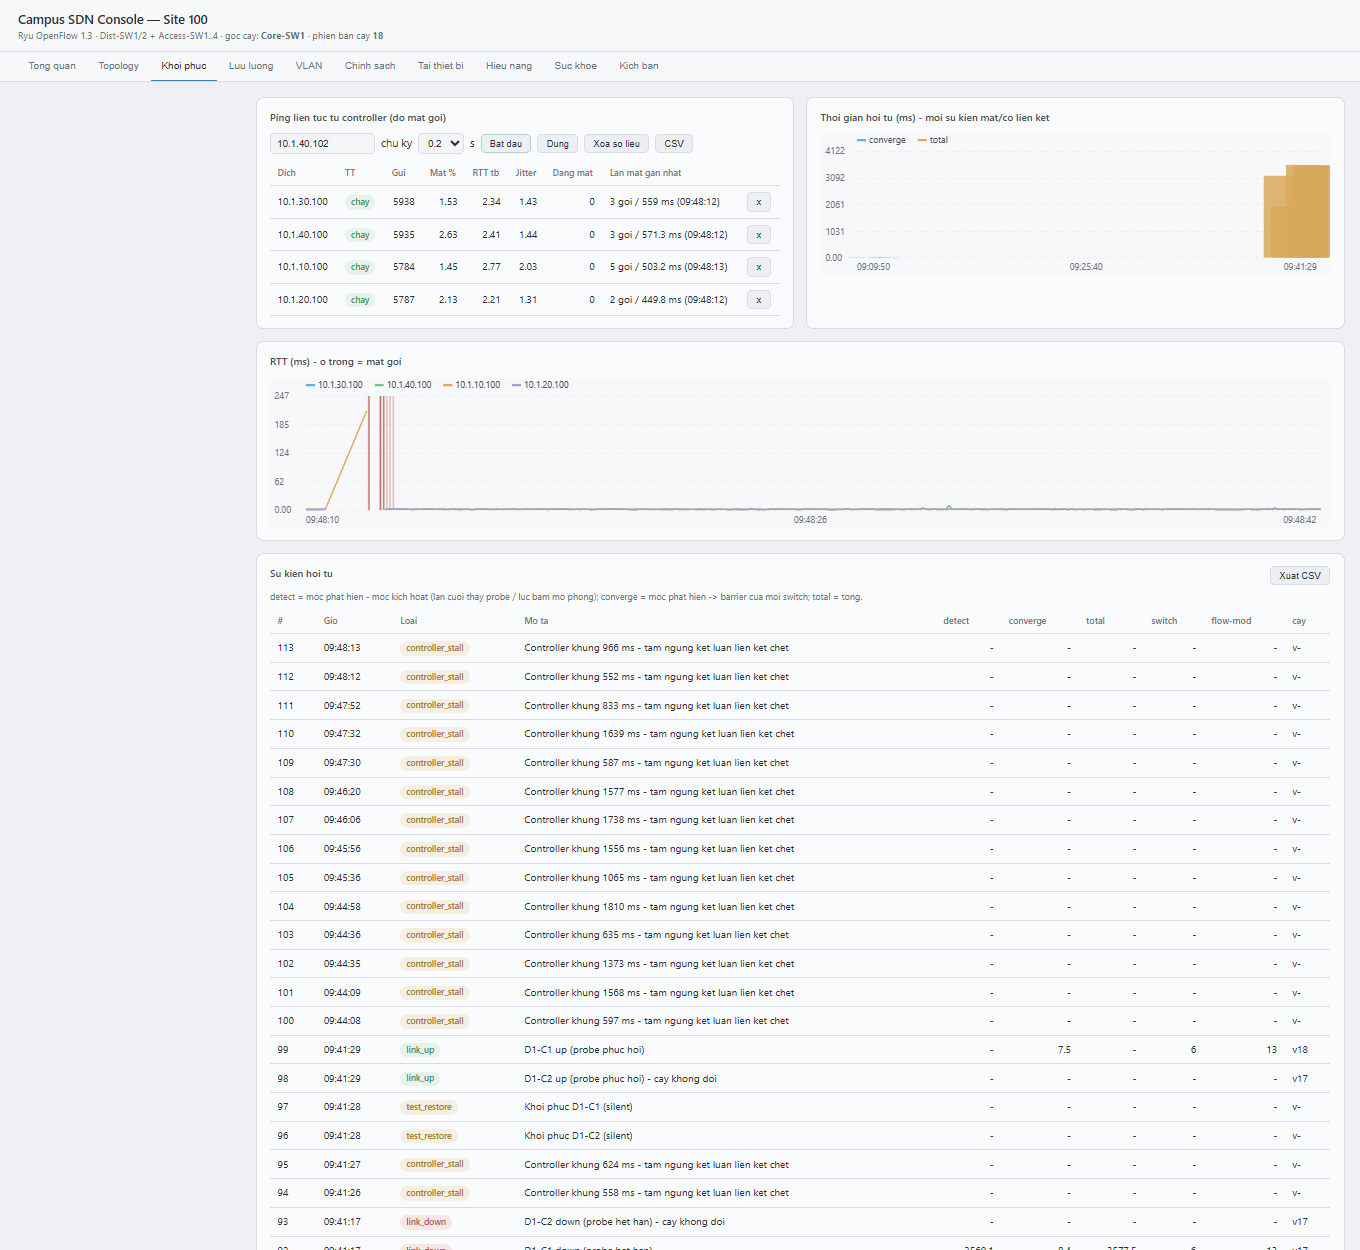
\includegraphics[width=\textwidth]{image/sdn-console-khoiphuc-20261108.png}
    \caption[Trang Khôi phục: ping liên tục và nhật ký sự kiện hội tụ]{Trang Khôi phục: ping liên tục tới bốn VLAN và nhật ký sự kiện \texttt{link\_down}/\texttt{link\_up} với thời gian phát hiện và hội tụ}
    \label{fig:console_khoiphuc}
\end{figure}

\textbf{Đo dưới tải cao:} VPCS chỉ sinh vài trăm kbit/s nên nhóm dùng các \textit{network namespace} trên máy chủ, gắn trực tiếp vào cổng Access, Server Farm, DMZ và LAN chi nhánh để đóng vai máy trạm chạy iperf3. Mỗi phép đo kéo dài 15--20 giây; song song, công cụ ping Controller qua VLAN 99 (5 gói/giây) và đọc tải qua REST để biết mặt phẳng điều khiển có bị ảnh hưởng không. Công cụ tự dừng nếu mất gói quá 60\% hoặc Controller mất switch. Kết quả ở Bảng~\ref{tab:sdn_tai_cao}.

\begin{table}[H]
    \centering
    \small
    \caption{Thông lượng dưới tải cao giữa các máy trạm}
    \label{tab:sdn_tai_cao}
    \begin{tabularx}{\textwidth}{|P{4.5cm}|P{3.4cm}|Y|}
        \hline
        \textbf{Đường đo} & \textbf{TCP, 3 lần (Mbit/s)} & \textbf{UDP: tốc độ phát $\rightarrow$ mất gói} \\
        \hline
        Cùng VLAN, cùng Access & 1184--1265 (TB 1214) & 50--500 Mbit/s $\rightarrow$ 0\% (3 lần mỗi mức) \\
        \hline
        Liên VLAN qua Core (VLAN 10 tới 40) & 165--173 (TB 170), khoảng 4100 gói gửi lại mỗi lần & 10--100 Mbit/s $\rightarrow$ tối đa 0,07\% (3 lần mỗi mức) \\
        \hline
        VLAN 10 tới Server Farm & 180--220 (TB 203), khoảng 4000 gói gửi lại mỗi lần & 5--50 Mbit/s $\rightarrow$ tối đa 0,05\% (3 lần mỗi mức) \\
        \hline
        VLAN 10 tới DMZ, qua ASAv & 0,08 & 0,1 Mbit/s $\rightarrow$ 0\%; 0,2 $\rightarrow$ 47\%; 0,5 $\rightarrow$ 79\% \\
        \hline
        Máy trạm chi nhánh tới chi nhánh (Site 200 tới 300, 300 tới 400, 500 tới 200), qua Brand-FW và overlay & Khoảng 0,09 & 0,1 Mbit/s $\rightarrow$ 0\%; 0,5 $\rightarrow$ 78\% \\
        \hline
    \end{tabularx}
\end{table}

Có ba nhận xét. Thứ nhất, dữ liệu không ảnh hưởng mặt phẳng điều khiển: trong toàn bộ 64 phép đo, ping Controller nhận 6321/6321 gói, RTT lớn nhất 325~ms, packet-in giữ quanh 85 gói/giây, luôn 6/6 switch và 13/13 liên kết. Thứ hai, OVS cùng Access không phải giới hạn ở các mức đã thử; đường liên VLAN giới hạn ở khoảng 170 Mbit/s, nhiều khả năng do Core IOL chuyển mạch bằng phần mềm (tiến trình Core-SW1 lên tới 60\% CPU, nhưng chưa tách riêng được khỏi phần OVS). Thứ ba, mọi đường qua tường lửa đều dừng ở khoảng 0,1~Mbit/s do ASAv chưa có giấy phép (\texttt{show version} báo \textit{Unlicensed}); tải trang HTTPS 50~kB từ VLAN 10, Site 200 hay Site 500 đều đạt khoảng 10--18~kB/s. Con số này là giới hạn của môi trường, không phải năng lực của thiết kế.

\begin{figure}[H]
    \centering
    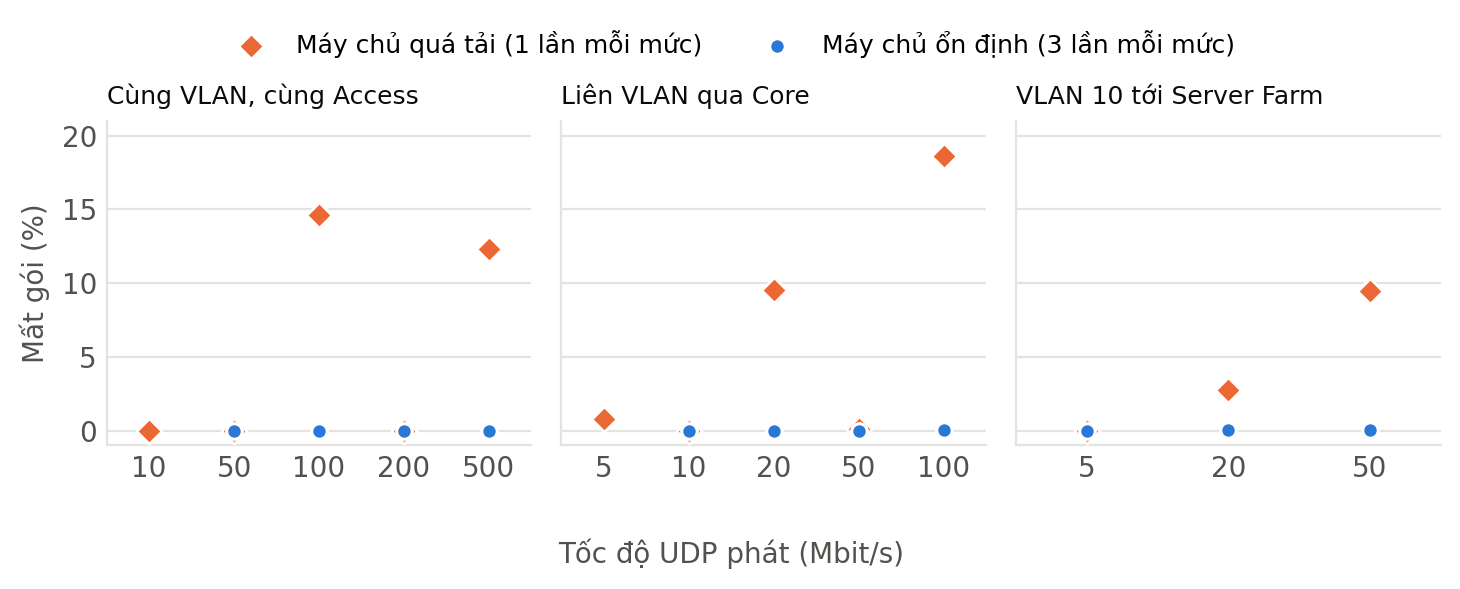
\includegraphics[width=0.95\textwidth]{image/bd-sdn-udp-haitrangthai.png}
    \caption{Mất gói UDP trên cùng cấu hình SDN ở hai trạng thái máy chủ}
    \label{fig:bd_udp_hai}
\end{figure}

\textbf{Ảnh hưởng của máy chủ ảo hóa:} cùng cấu hình và cùng phép đo được thực hiện ở hai trạng thái (Hình~\ref{fig:bd_udp_hai}). Khi máy chủ quá tải (load tới 42, đỉnh RTT VLAN 99 tới 631~ms), mất gói UDP thất thường và không tăng theo tốc độ: 14,6\% ở 100~Mbit/s nhưng 0\% ở 200~Mbit/s; các lần mất đều trùng đỉnh trễ. Khi máy chủ ổn định (load 10--15), mất gói gần như bằng 0 ở mọi mức, nên phần mất trước đó không phản ánh giới hạn của SDN. Đây là tương quan qua hai đợt đo, chưa xác định được cụ thể tài nguyên nào của máy chủ gây quá tải.

\begin{figure}[H]
    \centering
    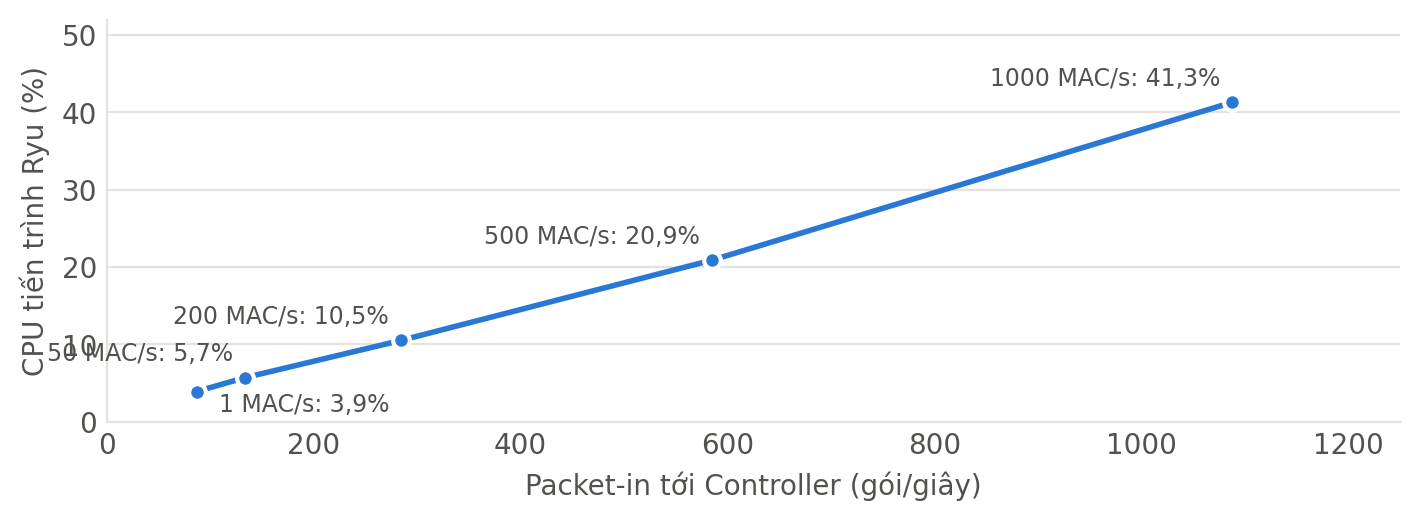
\includegraphics[width=0.85\textwidth]{image/bd-sdn-packetin.png}
    \caption{CPU của Ryu theo tải packet-in (20 giây mỗi mức)}
    \label{fig:bd_packetin}
\end{figure}

\textbf{CPU và RAM:} lấy mẫu mỗi 30 giây từ máy chủ, theo từng tiến trình node, qua ba trạng thái: rảnh (30 mẫu), tải SDN (40 mẫu), tải WAN (17 mẫu); kết quả ở Bảng~\ref{tab:cpu_ram}. Cách đo này cần thiết vì CPU do chính Core IOL báo cáo luôn là 0\%, cả qua SNMP lẫn \texttt{show processes cpu}, kể cả khi đang chuyển 336~Mbit/s, nên số liệu CPU Core trên Console không phản ánh tải chuyển mạch. vEdge chạy 2 vCPU chiếm ổn định hơn một lõi (khoảng 107\%) ngay cả lúc rảnh, trong khi vEdge2 Site 200 chạy 1 vCPU chỉ khoảng 8\%, cho thấy phần lớn CPU đó không tỷ lệ với lưu lượng.

\begin{table}[H]
    \centering
    \small
    \caption{CPU và RAM theo tiến trình node nhìn từ máy chủ (CPU 100\% tương ứng một lõi)}
    \label{tab:cpu_ram}
    \begin{tabularx}{\textwidth}{|Y|c|c|c|c|}
        \hline
        \textbf{Node} & \textbf{Rảnh, TB (\%)} & \textbf{Tải SDN, TB (\%)} & \textbf{Tải SDN, tối đa (\%)} & \textbf{RAM (MB)} \\
        \hline
        Core-SW1 / Core-SW2 & 3,7 / 0,9 & 15,1 / 0,9 & 60,4 / 1,0 & 218 \\
        \hline
        Dist-SW1 / Dist-SW2 & 11,4 / 11,2 & 26,5 / 12,2 & 84,0 / 26,8 & 969 / 919 \\
        \hline
        Access-SW1 / Access-SW4 & 7,2 / 7,0 & 26,0 / 13,3 & 78,7 / 47,8 & 944 / 911 \\
        \hline
        SDN Controller & 7,9 & 8,9 & 21,9 & 944 \\
        \hline
        FW-ASAv Site 100 (mỗi đơn vị) & 13,0 & 13,3 & 23,6 & 1526 \\
        \hline
        vEdge 2 vCPU (mỗi vEdge) & 107,5 & 108,5 & 135,0 & 960 \\
        \hline
        vManage & 38,8 & 49,3 & 229,6 & 32\,510 \\
        \hline
        Toàn bộ 69 node & 1052 & 1145 & 1801 & 81\,GB \\
        \hline
    \end{tabularx}
\end{table}

Toàn bộ lab chiếm khoảng 22\% năng lực CPU máy chủ (48 luồng) lúc rảnh, tối đa 38\% khi tải SDN.

\textbf{Hạn chế:} Controller vẫn có lúc bị khựng khi máy chủ ảo hóa chịu tải cao (nhận định từ tương quan thời gian, chưa chứng minh trực tiếp). Khi máy chủ ổn định, trang Sức khỏe ghi 5--7 lần khựng mỗi giờ, lâu nhất khoảng 1 giây; khi máy chủ quá tải là 69 lần mỗi giờ (0,5--4,2 giây). Cơ chế ân hạn giữ cho các sự kiện này không bị báo nhầm thành liên kết chết, nhưng chúng làm tăng RTT trung bình và gây mất lẻ tẻ gói đầu tiên của luồng mới (Bảng~\ref{tab:sdn_muc_tieu}).

\subsection{Triển khai mạng LAN tại các cơ sở phụ}

Khối lệnh~\ref{lst:brandfw_ch4} trích cấu hình Brand-FW Site 200; hai chi nhánh còn lại dùng cùng khuôn với địa chỉ và VLAN riêng.

\begin{lstlisting}[style=customcode,caption={Trích cấu hình Brand-FW Site 200},label={lst:brandfw_ch4}]
interface GigabitEthernet0/0.60
 vlan 60
 nameif vlan60
 security-level 100
 ip address 10.2.60.1 255.255.255.0
interface GigabitEthernet0/1
 nameif outside1
 security-level 0
 ip address 10.2.1.1 255.255.255.252
access-list SDWAN_IN extended permit ip 10.0.0.0 255.0.0.0 10.2.0.0 255.255.0.0
access-group SDWAN_IN in interface outside1
access-group SDWAN_IN in interface outside2
access-list VLAN99_IN extended permit ip 10.2.99.0 255.255.255.0 10.0.0.0 255.0.0.0
access-list VLAN99_IN extended deny ip any any log warnings
access-group VLAN99_IN in interface vlan99
route outside1 10.0.0.0 255.0.0.0 10.2.1.2 1 track 1
route outside2 10.0.0.0 255.0.0.0 10.2.1.6 2
route outside2 0.0.0.0 0.0.0.0 10.2.1.6 1 track 2
route outside1 0.0.0.0 0.0.0.0 10.2.1.2 2
dhcpd dns 10.1.90.10
dhcpd domain campus.internal
dhcpd address 10.2.60.100-10.2.60.199 vlan60
dhcpd enable vlan60
\end{lstlisting}

Các switch chi nhánh là IOL lớp 2: SwitchBrand có trunk lên Brand-FW mang hai VLAN nghiệp vụ và VLAN 99, hai trunk xuống switch khối, mỗi trunk chỉ mang VLAN của khối đó và VLAN 99; switch khối có hai cổng access. Sau khi khởi động, cấu hình của mọi switch được xác minh bằng \texttt{show vlan brief}, \texttt{show interfaces trunk} và lưu bằng \texttt{write memory}.

Kết quả cấp phát DHCP được tổng hợp trong Bảng~\ref{tab:dhcp_chi_nhanh_ch4}. Mọi địa chỉ nhận được đều nằm trong dải \texttt{.100--.199}, gateway là sub-interface \texttt{.1} của Brand-FW, DNS \texttt{10.1.90.10} và tên miền tìm kiếm \texttt{campus.internal}.

\begin{table}[H]
    \centering
    \scriptsize
    \caption{Kết quả kiểm thử DHCP tại các cơ sở phụ}
    \label{tab:dhcp_chi_nhanh_ch4}
    \begin{tabularx}{\textwidth}{|c|c|P{2.4cm}|P{4.4cm}|Z|}
        \hline
        \textbf{Site} & \textbf{VLAN} & \textbf{Subnet} & \textbf{Máy trạm} & \textbf{Địa chỉ nhận được} \\
        \hline
        200 & 60 & 10.2.60.0/24 & PC-NongNghiep-S200-1, -2 & 10.2.60.100; 10.2.60.101 \\
        \hline
        200 & 70 & 10.2.70.0/24 & PC-YTe-S200-2; PC-YTe-S200 (Ubuntu) & 10.2.70.100; 10.2.70.103 \\
        \hline
        300 & 80 & 10.3.80.0/24 & PC-DuLich-S300-1, -2 & 10.3.80.100; 10.3.80.101 \\
        \hline
        300 & 90 & 10.3.90.0/24 & PC-TaiChinh-S300-2; PC-TaiChinh-S300 (Ubuntu) & 10.3.90.101; 10.3.90.103 \\
        \hline
        400 & 50 & 10.4.50.0/24 & PC-ThuySan-S400-1, -2 & 10.4.50.100; 10.4.50.101 \\
        \hline
        400 & 60 & 10.4.60.0/24 & PC-LuHanh-S400-2; PC-LuHanh-S400 (Ubuntu) & 10.4.60.100; 10.4.60.103 \\
        \hline
    \end{tabularx}
\end{table}

\subsection{Triển khai SD-WAN}

\subsubsection{Controller, PKI và underlay}

Ba controller được cấu hình với System-IP, Site-ID 900, \texttt{organization-name site-900} và địa chỉ vBond. vManage đóng vai trò CA của hệ thống. Mỗi vEdge được đưa vào fabric theo quy trình: cấu hình cơ sở (System-IP, Site-ID, tổ chức, vBond, giao diện WAN có \texttt{tunnel-interface}), tuyến tới controller, tạo CSR, ký bằng Root CA, cài chuỗi Root CA rồi cài chứng thư thiết bị, đăng ký cặp chassis/serial trên cả ba controller và xác minh kết nối điều khiển. Hình~\ref{fig:wan_edge_list} là danh sách WAN Edge trên vManage: mười mục đã gán hostname và System-IP, mục thứ mười một là token chưa gán thiết bị.

\begin{figure}[H]
    \centering
    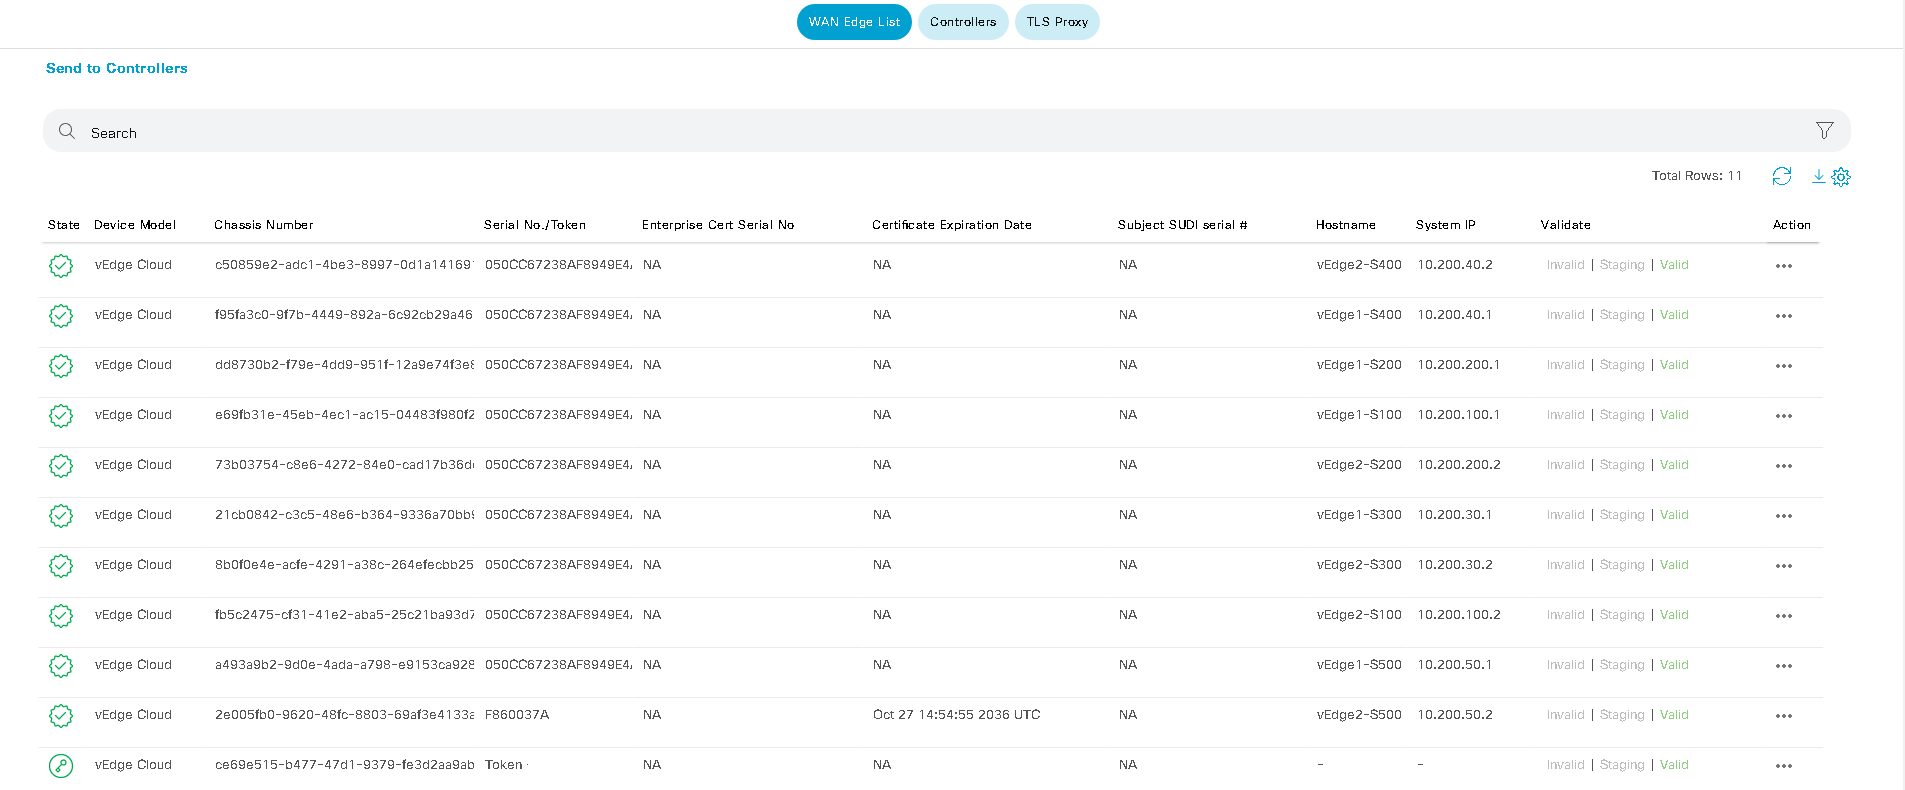
\includegraphics[width=\textwidth]{image/vmanage-wan-edge-list-20261107.png}
    \caption{Danh sách WAN Edge trên vManage: mười vEdge đã gán System-IP và một mục token chưa gán thiết bị, giá trị token đã được che}
    \label{fig:wan_edge_list}
\end{figure}

Underlay BGP được cấu hình trên hai router nhà cung cấp (Khối lệnh~\ref{lst:isp_ch4}) và trong VPN 0 của từng vEdge. Lệnh \texttt{default-originate} phải được khai báo trong \texttt{address-family ipv4} thì IOS mới gửi tuyến mặc định cho láng giềng.

\begin{lstlisting}[style=customcode,caption={Trích cấu hình BGP và NAT của router Internet},label={lst:isp_ch4}]
interface GigabitEthernet0/0
 ip address dhcp
 ip nat outside
interface GigabitEthernet0/5
 ip address 203.0.113.10 255.255.255.252
 ip nat inside
router bgp 64511
 bgp router-id 203.0.113.254
 neighbor 100.64.254.2 remote-as 64512
 neighbor 203.0.113.1 remote-as 65000
 neighbor 203.0.113.9 remote-as 65010
 address-family ipv4
  network 203.0.113.0 mask 255.255.255.252
  neighbor 100.64.254.2 activate
  neighbor 100.64.254.2 default-originate
  neighbor 100.64.254.2 prefix-list NO_DEFAULT_IN in
  neighbor 203.0.113.1 activate
  neighbor 203.0.113.1 default-originate
  neighbor 203.0.113.1 prefix-list NO_DEFAULT_IN in
 exit-address-family
ip nat inside source list NAT_ISP interface GigabitEthernet0/0 overload
ip route 10.9.0.0 255.255.0.0 203.0.113.249
ip prefix-list NO_DEFAULT_IN seq 5 deny 0.0.0.0/0
ip prefix-list NO_DEFAULT_IN seq 10 permit 0.0.0.0/0 le 32
\end{lstlisting}

\subsubsection{Cấu hình vEdge}

Khối lệnh~\ref{lst:vedge_ch4} trích cấu hình vEdge1-S100 (lược bỏ danh sách \texttt{allow-service}).

\begin{lstlisting}[style=customcode,caption={Trích cấu hình vEdge1-S100},label={lst:vedge_ch4}]
system
 host-name vEdge1-S100
 system-ip 10.200.100.1
 site-id 100
 organization-name site-900
 vbond 10.9.0.12
bfd app-route poll-interval 120000
vpn 0
 interface ge0/2
  ip address 100.64.100.1/30
  tunnel-interface
   encapsulation ipsec
   color mpls
 interface ge0/3
  ip address 203.0.113.1/30
  nat
  tunnel-interface
   encapsulation ipsec
   color biz-internet
 router bgp 65000
  neighbor 100.64.100.2 remote-as 64512
  neighbor 203.0.113.2 remote-as 64511
 ip route 10.9.0.0/24 100.64.100.2
 ip route 10.9.0.0/24 203.0.113.2
 ip route 0.0.0.0/0 100.64.100.2
 ip route 0.0.0.0/0 203.0.113.2
vpn 1
 name LAN
 router
  ospf
   area 0
    interface ge0/0
     hello-interval 2
     dead-interval  8
 interface ge0/0
  ip address 10.1.3.2/29
 interface loopback0
  ip address 10.1.255.1/32
 ip route 0.0.0.0/0 vpn 0
 omp
  advertise ospf external
omp
 advertise connected
 advertise static
\end{lstlisting}

\subsubsection{Các vấn đề kỹ thuật và nguyên nhân gốc}

\begingroup
\small
\begin{longtable}{|L{3.0cm}|L{5.2cm}|L{5.3cm}|}
    \caption{Các vấn đề SD-WAN, nguyên nhân gốc và cách khắc phục}\label{tab:loi_sdwan} \\
    \hline
    \textbf{Hiện tượng} & \textbf{Nguyên nhân gốc} & \textbf{Khắc phục} \\
    \hline
    \endfirsthead
    \hline
    \textbf{Hiện tượng} & \textbf{Nguyên nhân gốc} & \textbf{Khắc phục} \\
    \hline
    \endhead
    \hline
    \endfoot
    vEdge không xác minh được chứng thư & Thiếu chuỗi Root CA trên vEdge & Cài Root CA trước, chứng thư thiết bị sau \\
    \hline
    vBond/vSmart từ chối chứng thư dù đã ký đúng CA & Trường Organization của subject trong chứng thư không đúng giá trị nền tảng yêu cầu & Ký lại chứng thư với subject đúng chuẩn \\
    \hline
    vEdge lên vBond, vManage nhưng không có OMP với vSmart & Chưa đăng ký chassis/serial trên vSmart & Đăng ký trên đủ ba controller \\
    \hline
    Sau khi khởi động lại controller, một số vEdge rơi khỏi fabric & Danh sách thiết bị hợp lệ trên controller bị mất sau khởi động lại & Đăng ký lại; bổ sung bước kiểm tra danh sách đủ tám vEdge sau mỗi lần khởi động controller \\
    \hline
    Chỉ một color lên được controller (``1/3 vSmart'') & Tuyến \texttt{10.9.0.0/24} chỉ có qua MPLS, che tuyến \texttt{/16} qua Internet theo longest-prefix match & Khai báo tuyến \texttt{/24} qua cả hai transport (ECMP) \\
    \hline
    Mọi đường hầm chéo màu down tại chi nhánh & vEdge2 chi nhánh khai color \texttt{mpls} trên giao diện Internet & Sửa color thành \texttt{biz-internet} \\
    \hline
    BGP CE--PE không lên & Thiếu \texttt{allow-service bgp} trên tunnel-interface, thiếu \texttt{address-family} & Bổ sung cấu hình \\
    \hline
    Một TLOC mất hẳn kết nối điều khiển, OMP và BFD dù cấu hình không đổi (gặp ở vEdge2 Site 100 và vEdge1 Site 300) & Card mạng ảo của cổng WAN bị treo chiều nhận (bộ đếm drop của giao diện ảo trên máy chủ tăng liên tục) & \texttt{shutdown} / \texttt{no shutdown} cổng; BGP, TLOC, OMP và BFD lên lại \\
    \hline
    Đường hầm chéo màu của Site 100 down (biz-internet $\leftrightarrow$ mpls) & Mỗi TLOC chỉ có tuyến tới transport bên kia qua một cổng & Thêm tuyến mặc định qua từng transport trong VPN 0 của hai vEdge Site 100 \\
    \hline
    Overlay lên nhưng máy trạm các site không thông nhau & Chưa có VPN dịch vụ, cổng LAN nằm trong VPN 512 & Tạo VPN 1 \texttt{LAN}, chuyển cổng LAN vào VPN 1, thêm tuyến tổng hợp và quảng bá OMP \\
    \hline
    Mất MPLS tại chi nhánh làm mất 100\% gói, không tự phục hồi & Brand-FW không biết đường MPLS phía xa đã đứt nên vẫn đẩy lưu lượng về vEdge1; vEdge2 chuyển lưu lượng LAN qua vEdge1 nên chiều về đi vào cổng khác chiều đi và bị tường lửa trạng thái hủy & Brand-FW theo dõi beacon \texttt{10.1.255.1} bằng \texttt{sla monitor} và \texttt{track}; tuyến LAN của vEdge2 trỏ thẳng về \texttt{outside2}; control policy ưu tiên vEdge1 của mọi site \\
\end{longtable}
\endgroup

\subsubsection{Kết quả kiểm thử SD-WAN}

\begin{itemize}
    \item \textbf{Control plane:} ba controller và mười vEdge Site 100--500 đều reachable trên vManage (Hình~\ref{fig:vmanage_overview} và Hình~\ref{fig:vmanage_devices}). Mỗi vEdge Site 100 đạt 2/2 kết nối tới vSmart, mỗi vEdge chi nhánh đạt 1/1. Tại vEdge1-S100, mỗi color có một kết nối DTLS tới vSmart, riêng biz-internet có thêm kết nối tới vManage (Hình~\ref{fig:vmanage_control}).
    \item \textbf{Underlay:} mọi phiên eBGP CE--PE và phiên giữa hai nhà cung cấp ở trạng thái Established; các vEdge nhận tuyến mặc định qua transport tương ứng.
    \item \textbf{BFD:} toàn bộ phiên đều up --- mỗi vEdge Site 100 16/16, mỗi vEdge chi nhánh 10/10 (Hình~\ref{fig:vmanage_devices}); tổng các cột này là 112, bằng số đường hầm trên trang tổng quan. Cả năm site đạt BFD Full (Hình~\ref{fig:vmanage_health}). Hình~\ref{fig:bfd_s200} là đầu ra trên vEdge2 Site 200: mười phiên BFD tới các TLOC của Site 100, 300, 400, 500 đều up (timer mặc định 1000~ms $\times$ 7) và phiên OMP với vSmart ở trạng thái up.
    \item \textbf{Overlay dữ liệu:} ping giữa máy trạm các chi nhánh 200, 300, 400 thành công 10/10; máy trạm chi nhánh truy cập được dịch vụ tại Campus chính.
    \item \textbf{Chất lượng đường truyền:} thống kê app-route từ Site 200 đến Site 300 qua MPLS: mất gói 0\%, độ trễ 37~ms, jitter 6~ms --- thỏa \texttt{SLA\_REALTIME}. Trên vManage, trong 24 giờ, hai TLOC của vEdge1-S100 đều up, bảng TLOC ghi mất gói khoảng 0,2\%, độ trễ 18--20~ms, jitter 17--19~ms; biểu đồ có hai đỉnh mất gói 2--3\%, nguyên nhân chưa đối chiếu với nhật ký (Hình~\ref{fig:vmanage_tloc}).
    \item \textbf{Chính sách tập trung:} mọi vEdge nhận đúng chính sách từ vSmart (\texttt{show policy from-vsmart}). Để chứng minh chính sách được thực thi, nhóm xây dựng công cụ kiểm thử tự động: đọc bộ đếm của từng luật qua API của vManage, sinh lưu lượng thật từ máy trạm chi nhánh, rồi đọc lại bộ đếm. Chạy lần lượt từ máy trạm cả bốn chi nhánh (PC-YTe-S200-2, PC-TaiChinh-S300-2, PC-LuHanh-S400-2, VPC11 Site 500), mỗi nơi đều đạt 10/10 phép thử (Bảng~\ref{tab:kiem_thu_chinh_sach}).
    \item \textbf{Failover tại chi nhánh:} khi cắt MPLS hoặc mất vEdge1, Brand-FW phát hiện mất beacon qua \texttt{sla monitor}/\texttt{track} và chuyển lưu lượng nội bộ sang vEdge2 (Internet); khi cắt Internet hoặc mất vEdge2, lưu lượng ra Internet chuyển sang vEdge1 và thoát qua MPLS; khi nối lại, lưu lượng tự quay về. Nếu không có thiết kế beacon, chi nhánh mất 100\% gói và không tự phục hồi. Phép đo dùng cách cắt thật tại máy chủ (\texttt{ip link set <tap> down}, thiết bị không nhận sự kiện liên kết), lặp 46 lần trên cả bốn chi nhánh (Bảng~\ref{tab:failover_chi_nhanh}, Hình~\ref{fig:bd_failover_4site}), ICMP 5 gói/giây, đồng thời hai đầu đo: \textit{luồng mới} đổi ICMP id mỗi gói, \textit{luồng đang chạy} giữ nguyên id. Luồng mới khôi phục sau \textbf{3,2--13,4 giây}, không khác biệt đáng kể giữa các site. Luồng đang chạy khôi phục sau 18,6--38,1 giây. Khi nối lại liên kết, gián đoạn có trung vị 12 giây; 8/46 lần trên 20 giây, lâu nhất 41 giây.
    \item \textbf{Hai lỗi do phép đo failover phát hiện:} (1) ASA gắn kết nối vào đường ra cũ nên luồng đang chạy mất suốt thời gian cắt, dù luồng mới đã chuyển đường sau khoảng 8 giây; thêm \texttt{timeout floating-conn 0:00:30} trên bốn Brand-FW giải quyết được, đổi lại luồng đang chạy khôi phục chậm hơn luồng mới khoảng 15--30 giây. (2) Tại Site 500, khi cắt Internet, máy trạm mất Internet suốt 90 giây cắt vì cổng MPLS của vEdge1 thiếu lệnh \texttt{nat} so với ba chi nhánh kia; sau khi bổ sung, thời gian khôi phục còn 7,8--10,3 giây.
    \item \textbf{Failover transport tại Site 100:} khi tắt cổng MPLS trên cả hai vEdge Site 100, các đường hầm qua Internet tiếp tục mang lưu lượng; TLOC MPLS phục hồi khi bật lại cổng nhờ tuyến tới controller được khai báo qua cả hai transport.
    \item \textbf{AAR khi đường truyền suy giảm:} dùng \texttt{netem} tăng trễ 400~ms trên cổng MPLS của vEdge1 Site 100, trong khi Server Farm ping Site 200 5 gói/giây. Trễ của tunnel MPLS trong \texttt{show app-route stats} là trung bình trượt qua 6 chu kỳ 2 phút nên tăng dần, vượt ngưỡng 150~ms của \texttt{SLA\_REALTIME} sau khoảng 5,5 phút; lưu lượng trên tunnel chuyển từ \texttt{mpls} sang \texttt{biz-internet} trong khoảng 5,5--7 phút. Gỡ \texttt{netem}, lưu lượng tự quay về sau khoảng 10--11 phút. Toàn bộ quá trình chỉ mất 4/7578 gói (0,05\%). AAR chuyển đường êm nhưng chậm, nên chỉ phù hợp với suy giảm kéo dài; đứt hẳn vẫn dựa vào BFD và Brand-FW.
    \item \textbf{Timer BFD:} hệ thống dùng timer mặc định 1000~ms $\times$ 7; timer mới chỉ có hiệu lực khi cả hai đầu phiên cùng đổi. Thử 500~ms $\times$ 4 cho gián đoạn 3,4--6,7 giây ở 3 trong 5 lần, so với 7,7--8,3 giây của đường đối chứng, nhưng phiên với vEdge2 Site 200 (1 vCPU) tự rớt mỗi 15--60 giây khi không cắt liên kết, nên timer rút ngắn không được áp dụng.
    \item \textbf{Tách thời gian khôi phục theo từng chiều:} bắt gói đồng thời trên các cổng của Brand-FW và vEdge khi cắt MPLS của vEdge1 Site 200, đích là cổng outside của FW Site 100, được 4/5 lần hợp lệ. Gói trả lời về tới máy trạm sau 8,3--9,1 giây (trung bình 8,8 giây), ổn định qua các lần đo. Chiều đi dao động hơn: Brand-FW chuyển sang vEdge2 sau 3,4--7,7 giây, tức sau 2--4 lần thăm dò SLA thất bại. Có lần chiều đi xong sau 3,43 giây, Site 100 trả lời ngay nhưng gói trả lời vẫn mất 5,2 giây mới về tới Site 200. Vì vậy giới hạn chính là chiều về, chờ BFD mặc định 7 giây để Site 100 bỏ đường cũ; chiều đi là giới hạn thứ hai. Muốn giảm RTO phải giảm cả timer BFD ở hai site lẫn chu kỳ SLA trên Brand-FW (Hình~\ref{fig:bd_failover}).
    \item \textbf{Site 500:} VPC11 nhận DHCP \texttt{10.5.10.100} và ping gateway 20/20. Máy trạm Site 500 thông Site 200, 300, 400, Server Farm, Web Server và Internet. Đo nền 5 phút (1500 gói, máy chủ ổn định): tới Site 200 mất 0\%, RTT trung vị 4~ms, phân vị 95 là 5~ms; tới Server Farm mất 0\%, 7~ms và 31~ms; để đối chứng, Site 200 tới Site 300 cũng mất 0\%, 5~ms và 10~ms. Lượt đo trước đó ghi mất 2,75\% và RTT gần 1 giây; khi máy chủ quá tải, đo đối chứng cho thấy các cặp site khác cũng tăng RTT tương tự (trung bình 116--233~ms) nên đây là hiện tượng chung do máy chủ, không phải lỗi riêng của Site 500. Failover của Site 500 có trong Bảng~\ref{tab:failover_chi_nhanh}.
    \item \textbf{Thông lượng liên site:} đo bằng \texttt{tools iperf} giữa các vEdge trong VPN~1, không qua tường lửa, được 13/15 chiều (giữa máy trạm, qua tường lửa, xem Bảng~\ref{tab:sdn_tai_cao}). TCP trung bình 1,95~Mbit/s (1,66--2,20) giữa các vEdge1 và 1,73~Mbit/s ở hai chiều vEdge2 về Site 100. UDP 2~Mbit/s gần như không mất gói, 3~Mbit/s mất khoảng 14\%, 10~Mbit/s mất khoảng 81\%. Hai vEdge cùng site nối trực tiếp đạt 50~Mbit/s không mất gói, nên đây là giới hạn của WAN mô phỏng (nghi do router nhà cung cấp chạy vIOS, chưa chứng minh), không phản ánh năng lực SD-WAN (Hình~\ref{fig:bd_udp} và Hình~\ref{fig:bd_tcp}).
\end{itemize}

\begin{table}[H]
    \centering
    \small
    \caption{Thời gian khôi phục khi cắt thật tại chi nhánh, giây: nhỏ nhất--lớn nhất (trung bình), số lần trong ngoặc vuông}
    \label{tab:failover_chi_nhanh}
    \begin{tabularx}{\textwidth}{|P{1.75cm}|Y|Y|Y|Y|P{1.75cm}|}
        \hline
        \textbf{Kịch bản} & \textbf{Site 200} & \textbf{Site 300} & \textbf{Site 400} & \textbf{Site 500} & \textbf{Luồng đang chạy} \\
        \hline
        Cắt MPLS & 7,8--10,0 (8,5) [5] & 7,9--8,5 (8,2) [3] & 8,1--8,5 (8,3) [3] & 7,8--11,2 (8,9) [5] & 32,5--38,1 \\
        \hline
        Mất vEdge1 & 8,7 (8,7) [2] & 7,8--8,4 (8,1) [2] & 8,3--8,7 (8,5) [2] & 7,4--10,0 (8,4) [3] & 32,9--36,6 \\
        \hline
        Cắt Internet & 7,2--11,1 (9,3) [3] & 9,1--11,8 (10,5) [3] & 11,3--13,2 (12,2) [3] & 7,8--10,3 (9,1) [3] & 22,6--28,6 \\
        \hline
        Mất vEdge2 & 3,2--4,8 (4,0) [2] & 4,7--13,4 (9,1) [2] & 8,8--10,2 (9,6) [2] & 6,0--8,4 (7,2) [3] & 18,6--28,9 \\
        \hline
    \end{tabularx}
\end{table}

Các cột site là luồng mới. Hai kịch bản đầu đo lưu lượng liên site, hai kịch bản sau đo lưu lượng ra Internet (8.8.8.8). Số lần lặp tại mỗi kịch bản từ 2 đến 5 nên chỉ cho biết khoảng dao động, chưa đủ để so sánh giữa các site.

\begin{figure}[H]
    \centering
    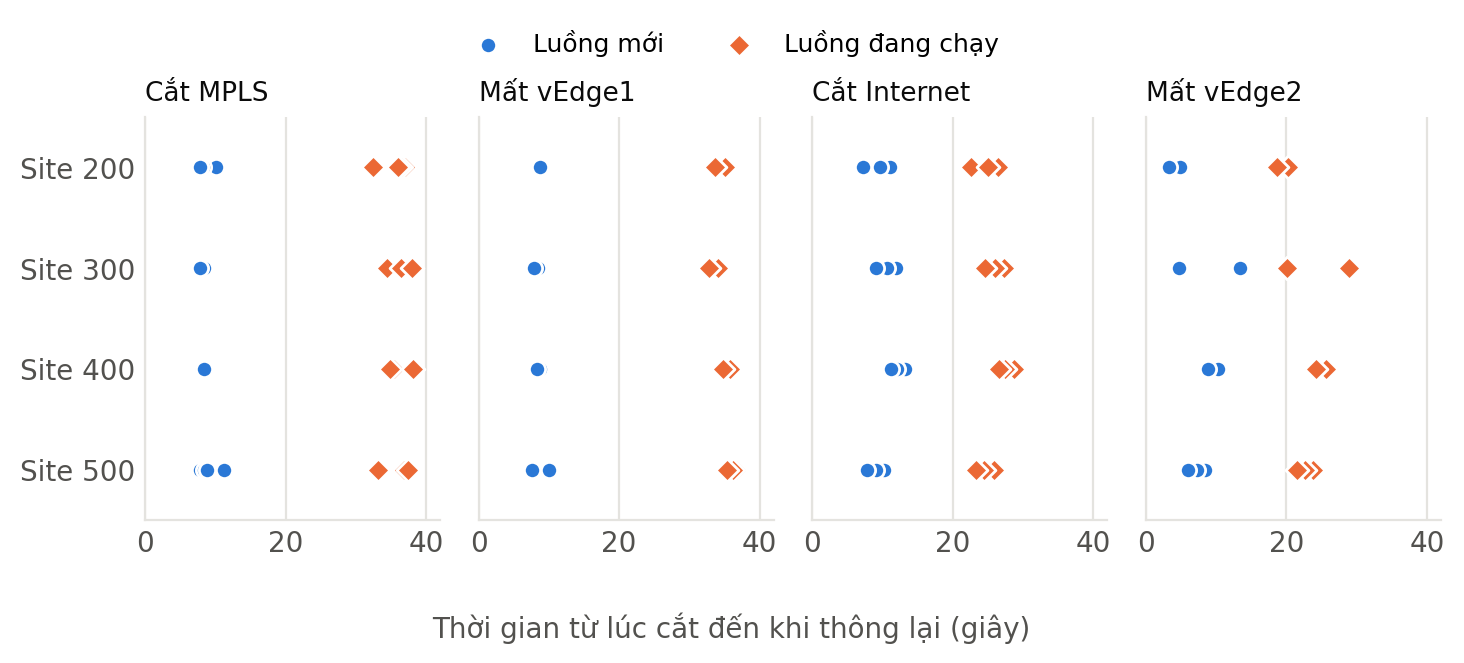
\includegraphics[width=\textwidth]{image/bd-failover-4site.png}
    \caption{Thời gian khôi phục từng lần cắt, theo site và kịch bản}
    \label{fig:bd_failover_4site}
\end{figure}

\begin{figure}[H]
    \centering
    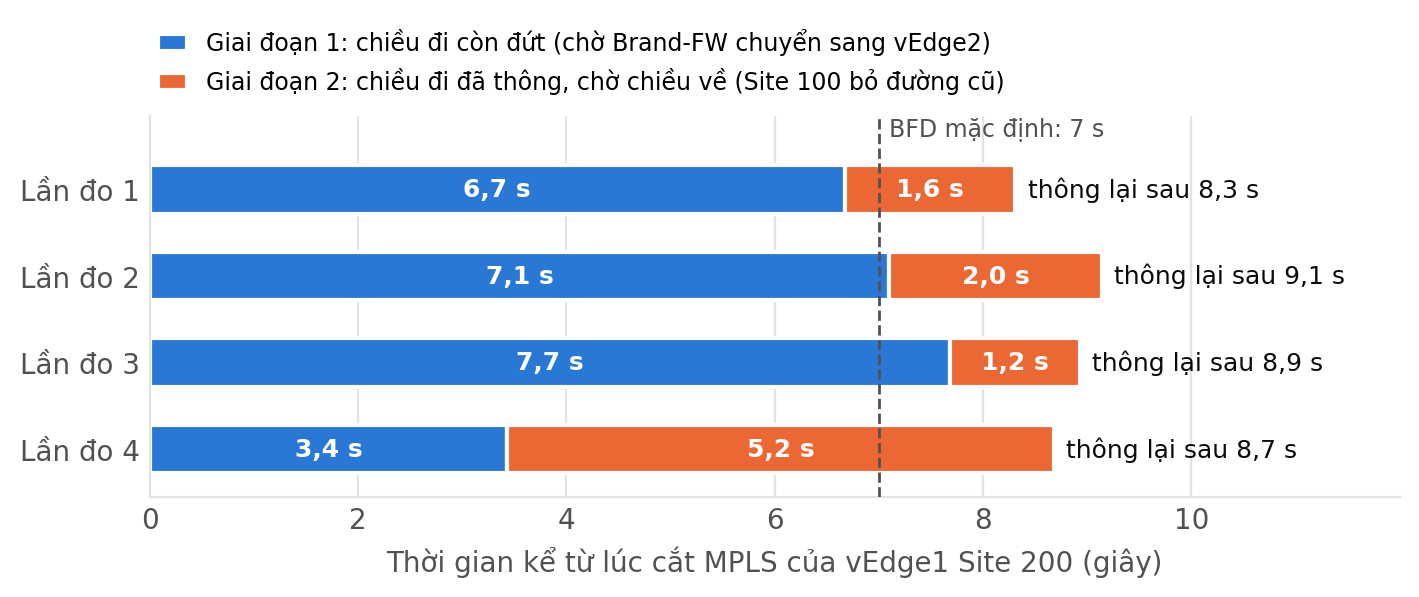
\includegraphics[width=0.95\textwidth]{image/bd-failover-2chieu.png}
    \caption{Thời gian khôi phục theo từng chiều khi cắt MPLS vEdge1 Site 200 (4 lần hợp lệ)}
    \label{fig:bd_failover}
\end{figure}

\begin{figure}[H]
    \centering
    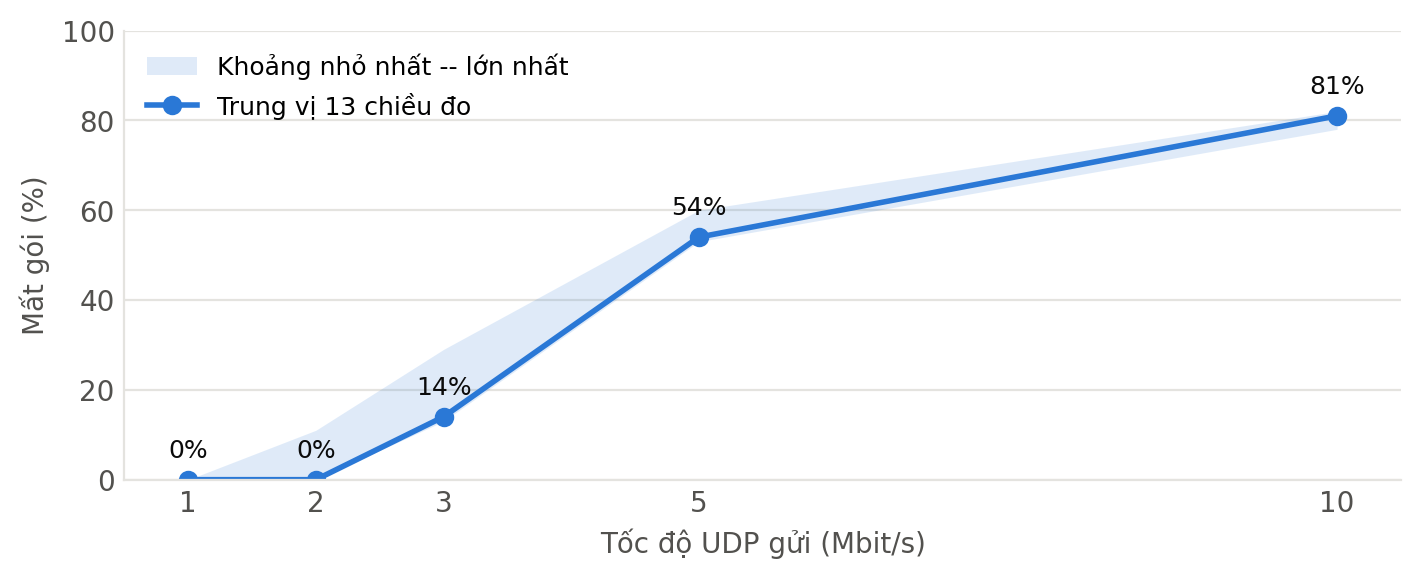
\includegraphics[width=0.9\textwidth]{image/bd-udp-matgoi.png}
    \caption{Tỷ lệ mất gói UDP theo tốc độ gửi giữa các vEdge}
    \label{fig:bd_udp}
\end{figure}

\begin{figure}[H]
    \centering
    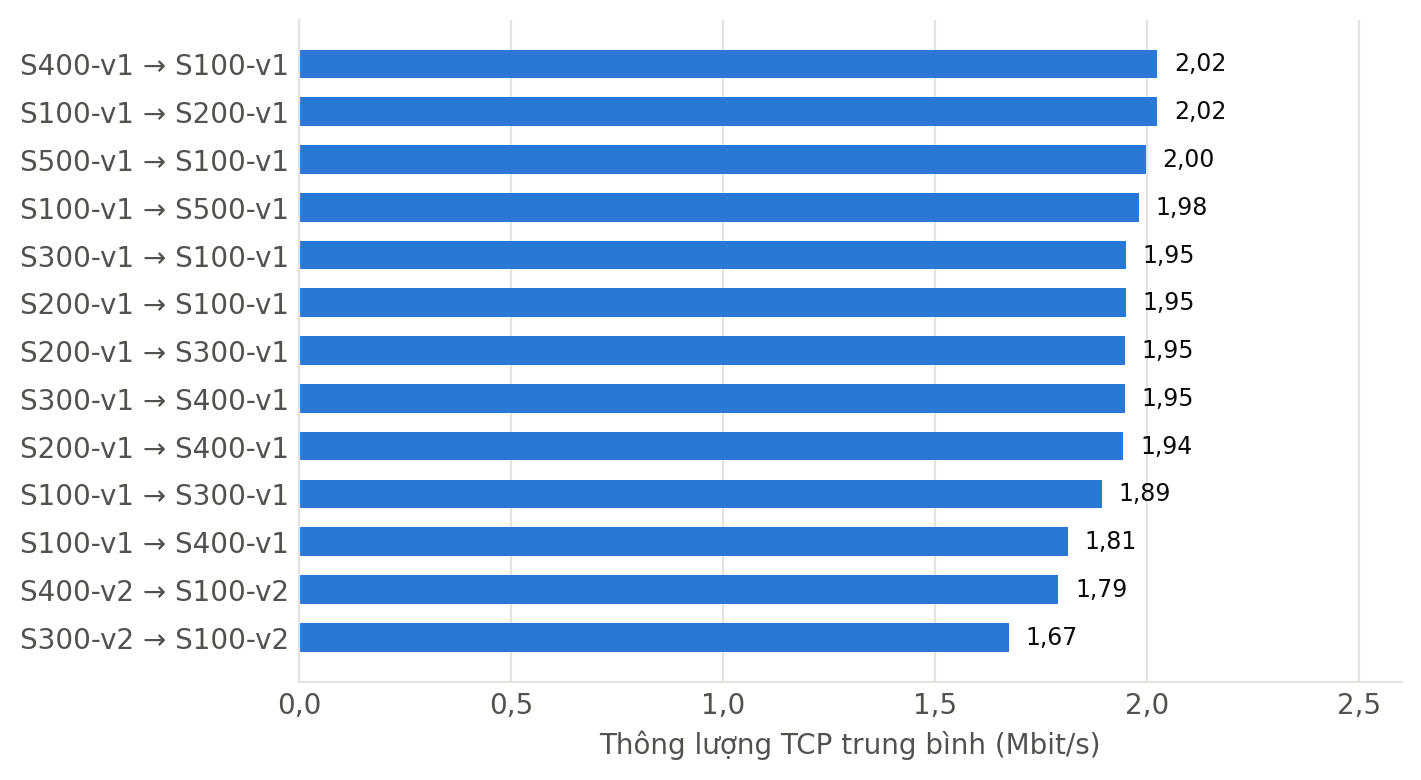
\includegraphics[width=0.9\textwidth]{image/bd-tcp-thongluong.png}
    \caption{Thông lượng TCP trung bình theo từng chiều đo giữa các vEdge}
    \label{fig:bd_tcp}
\end{figure}

\begin{figure}[H]
    \centering
    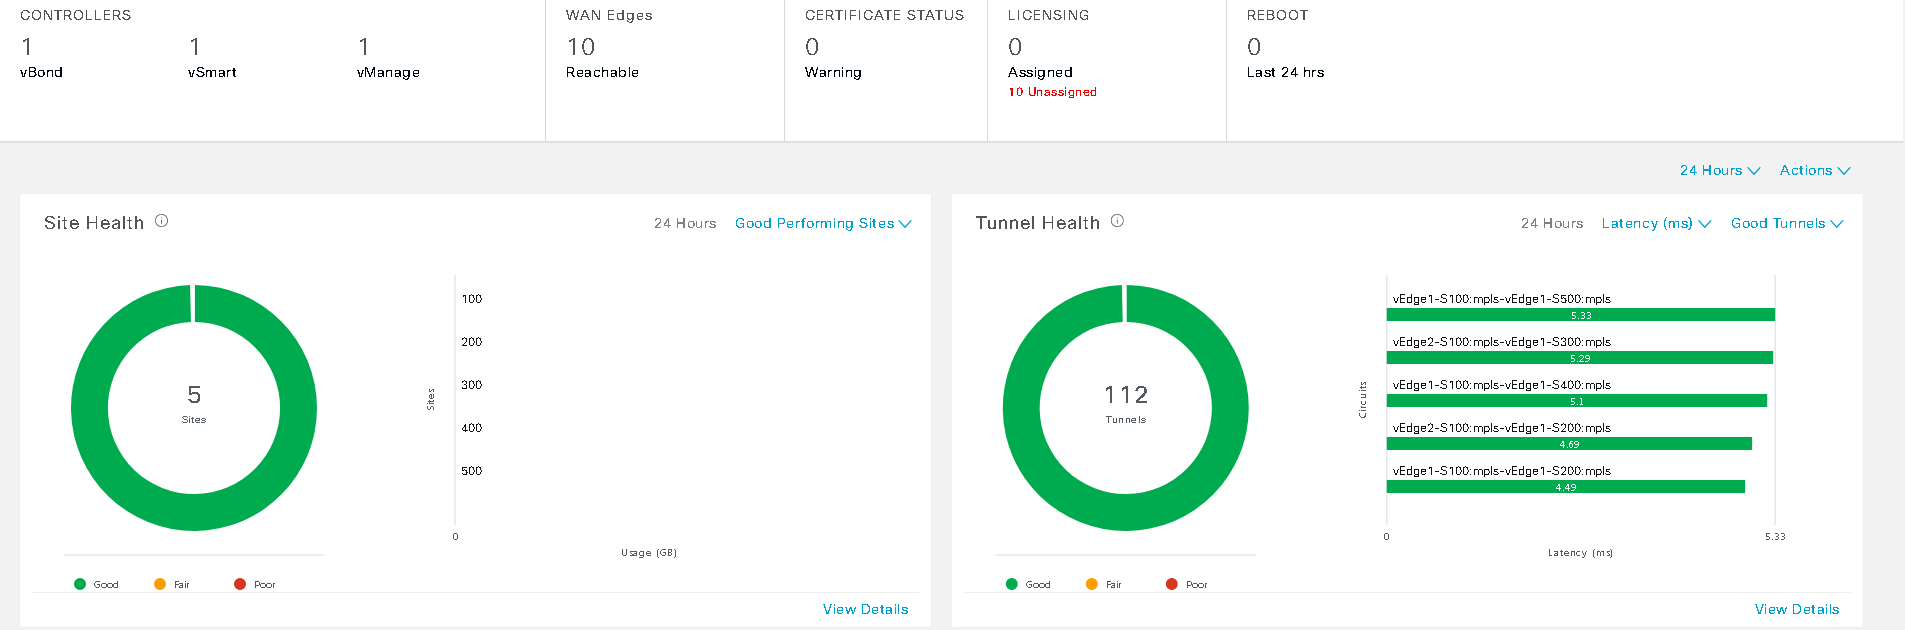
\includegraphics[width=\textwidth]{image/vmanage-overview-20261107.png}
    \caption{Trang tổng quan vManage: ba controller, mười WAN Edge reachable, năm site và 112 đường hầm ở mức tốt}
    \label{fig:vmanage_overview}
\end{figure}

\begin{figure}[H]
    \centering
    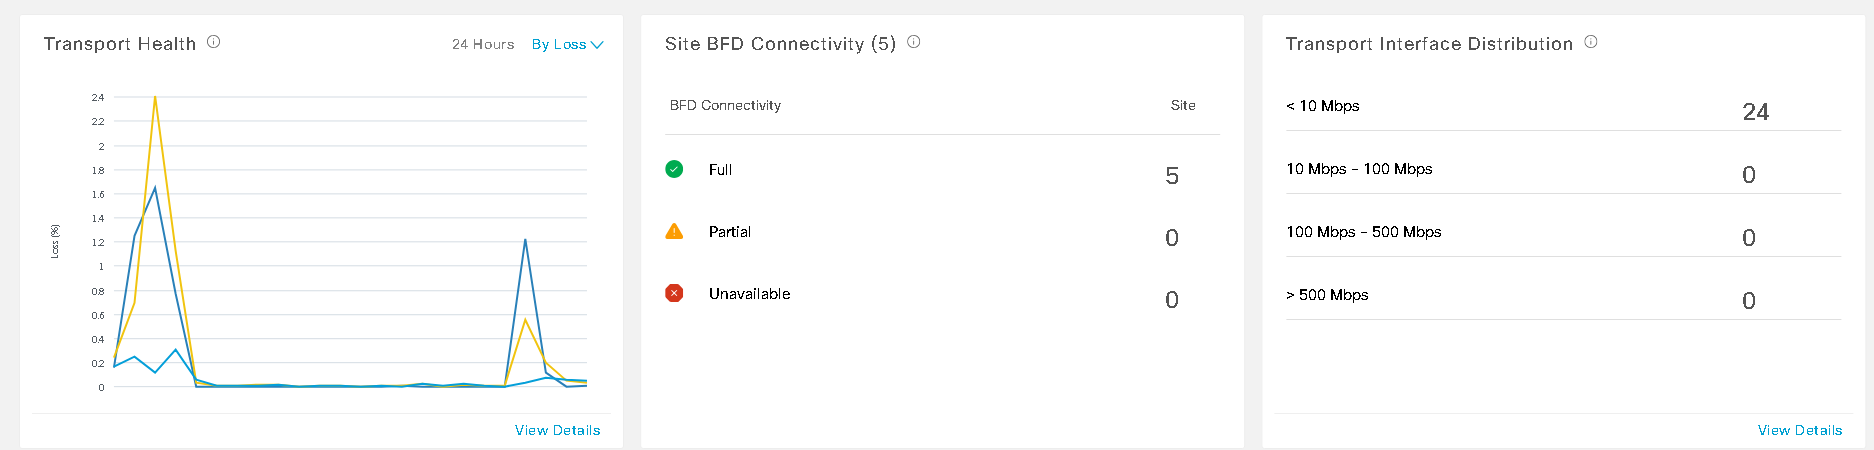
\includegraphics[width=\textwidth]{image/vmanage-health-20261107.png}
    \caption{vManage: mất gói theo transport trong 24 giờ, năm site đạt BFD Full và phân bố băng thông cổng transport}
    \label{fig:vmanage_health}
\end{figure}

\begin{figure}[H]
    \centering
    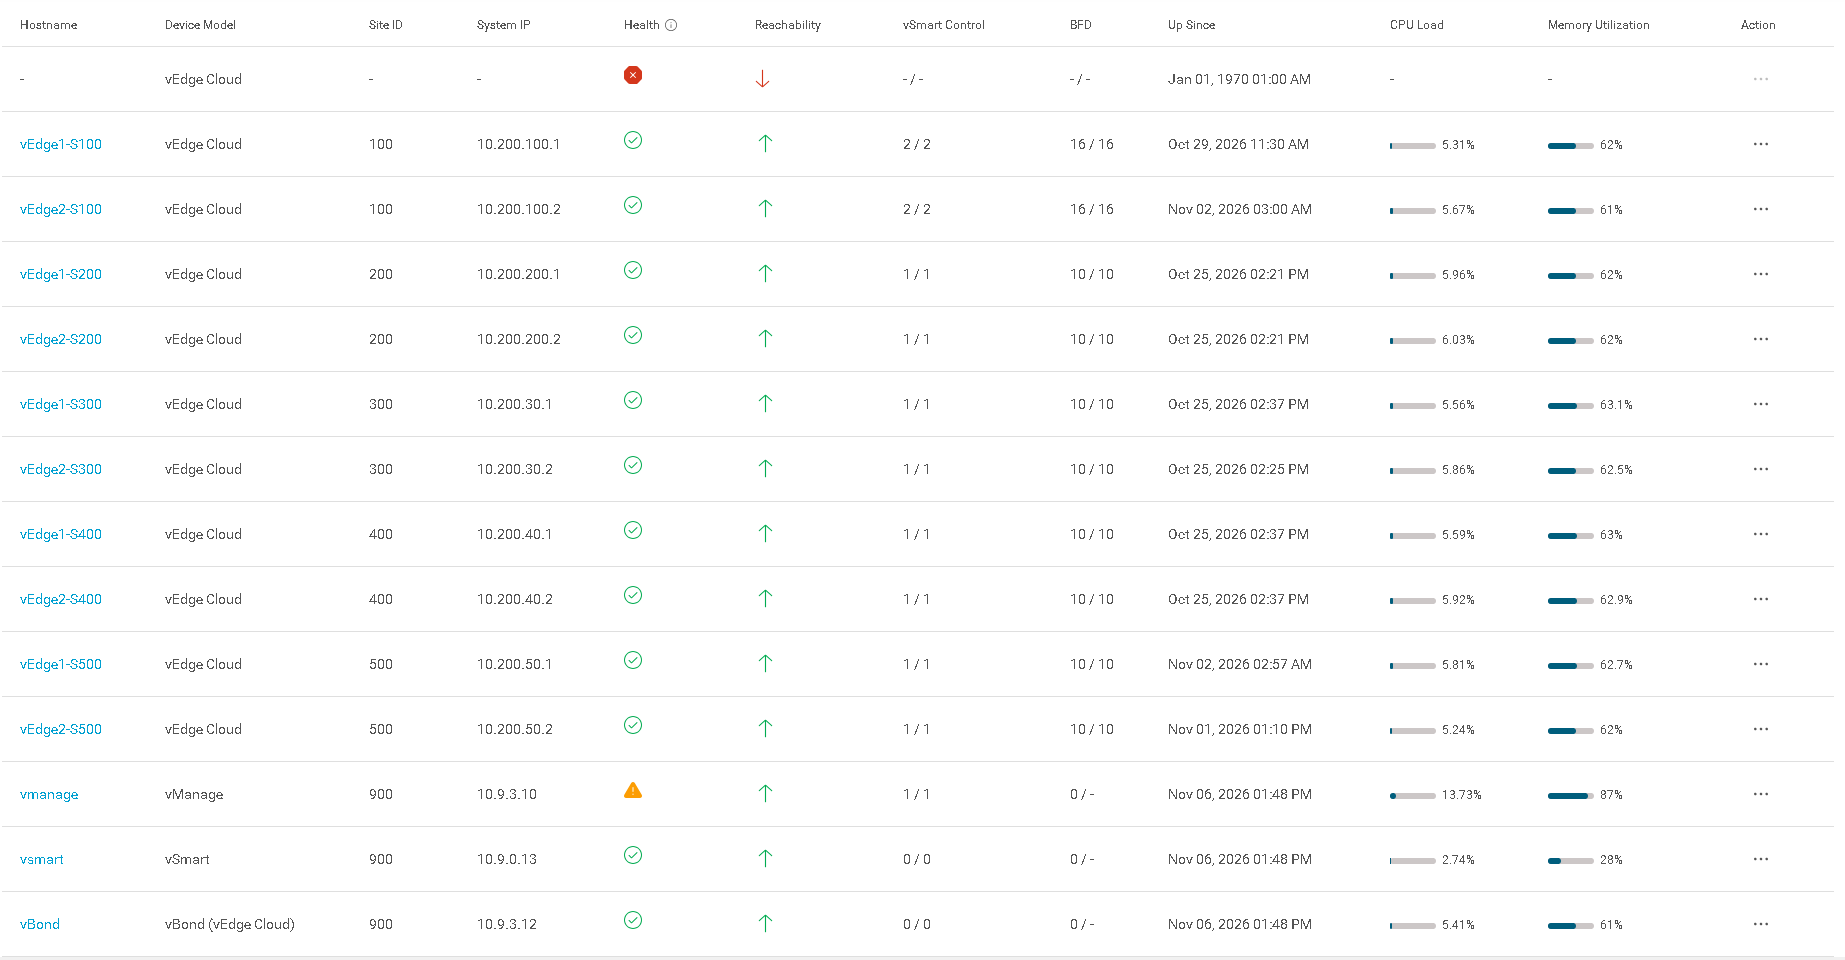
\includegraphics[width=\textwidth]{image/vmanage-devices-20261107.png}
    \caption{Danh sách thiết bị trên vManage. Dòng đầu không có tên là mục WAN Edge chưa gán thiết bị; vManage hiện cảnh báo vàng, bộ nhớ 87\%}
    \label{fig:vmanage_devices}
\end{figure}

\begin{figure}[H]
    \centering
    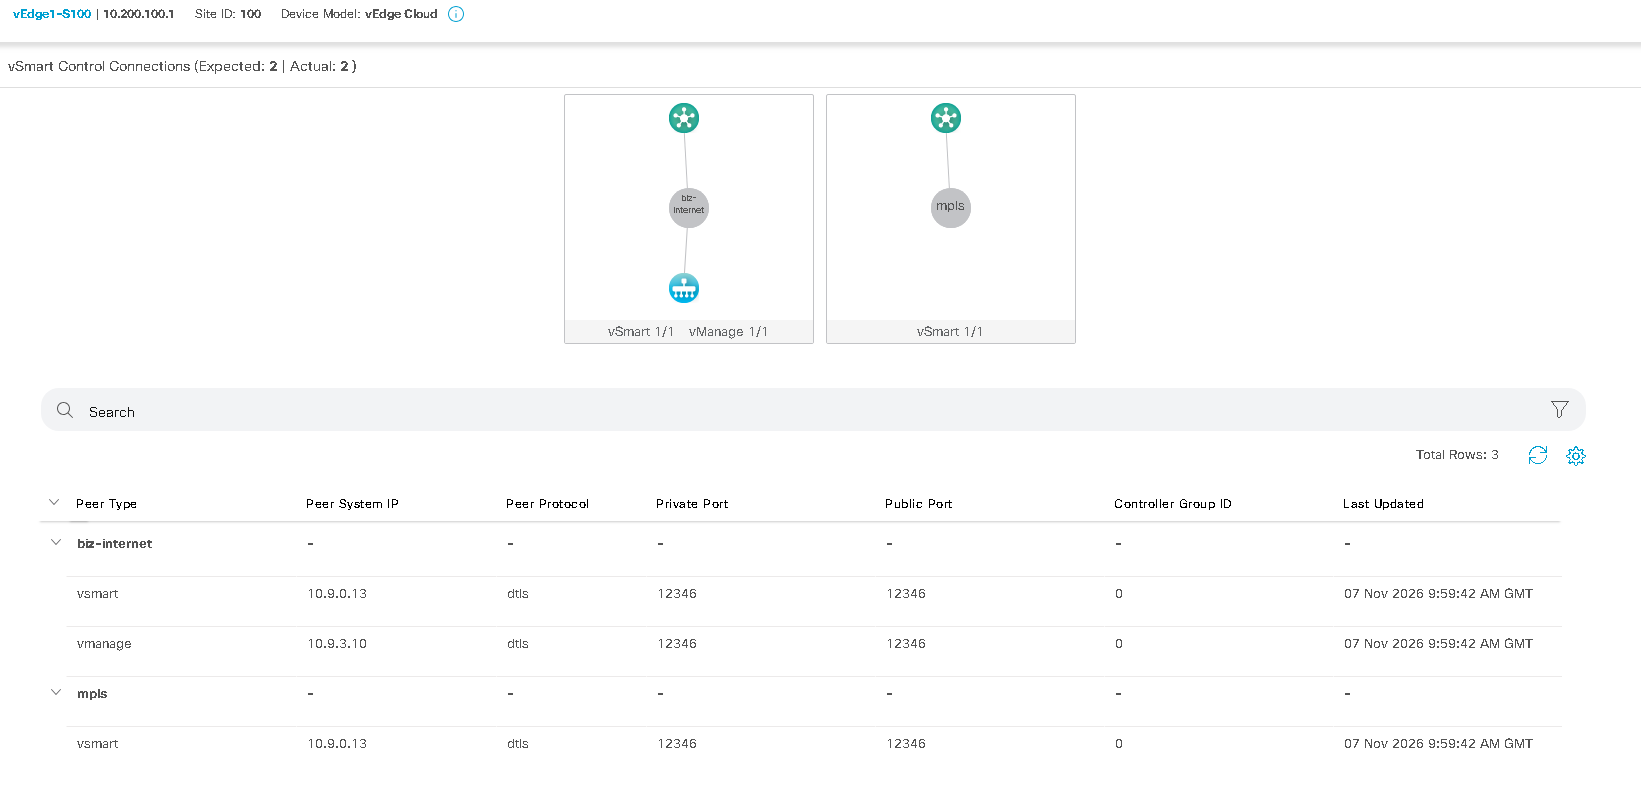
\includegraphics[width=\textwidth]{image/vmanage-control-s100-20261107.png}
    \caption{Kết nối điều khiển của vEdge1-S100 trên hai color}
    \label{fig:vmanage_control}
\end{figure}

\begin{figure}[H]
    \centering
    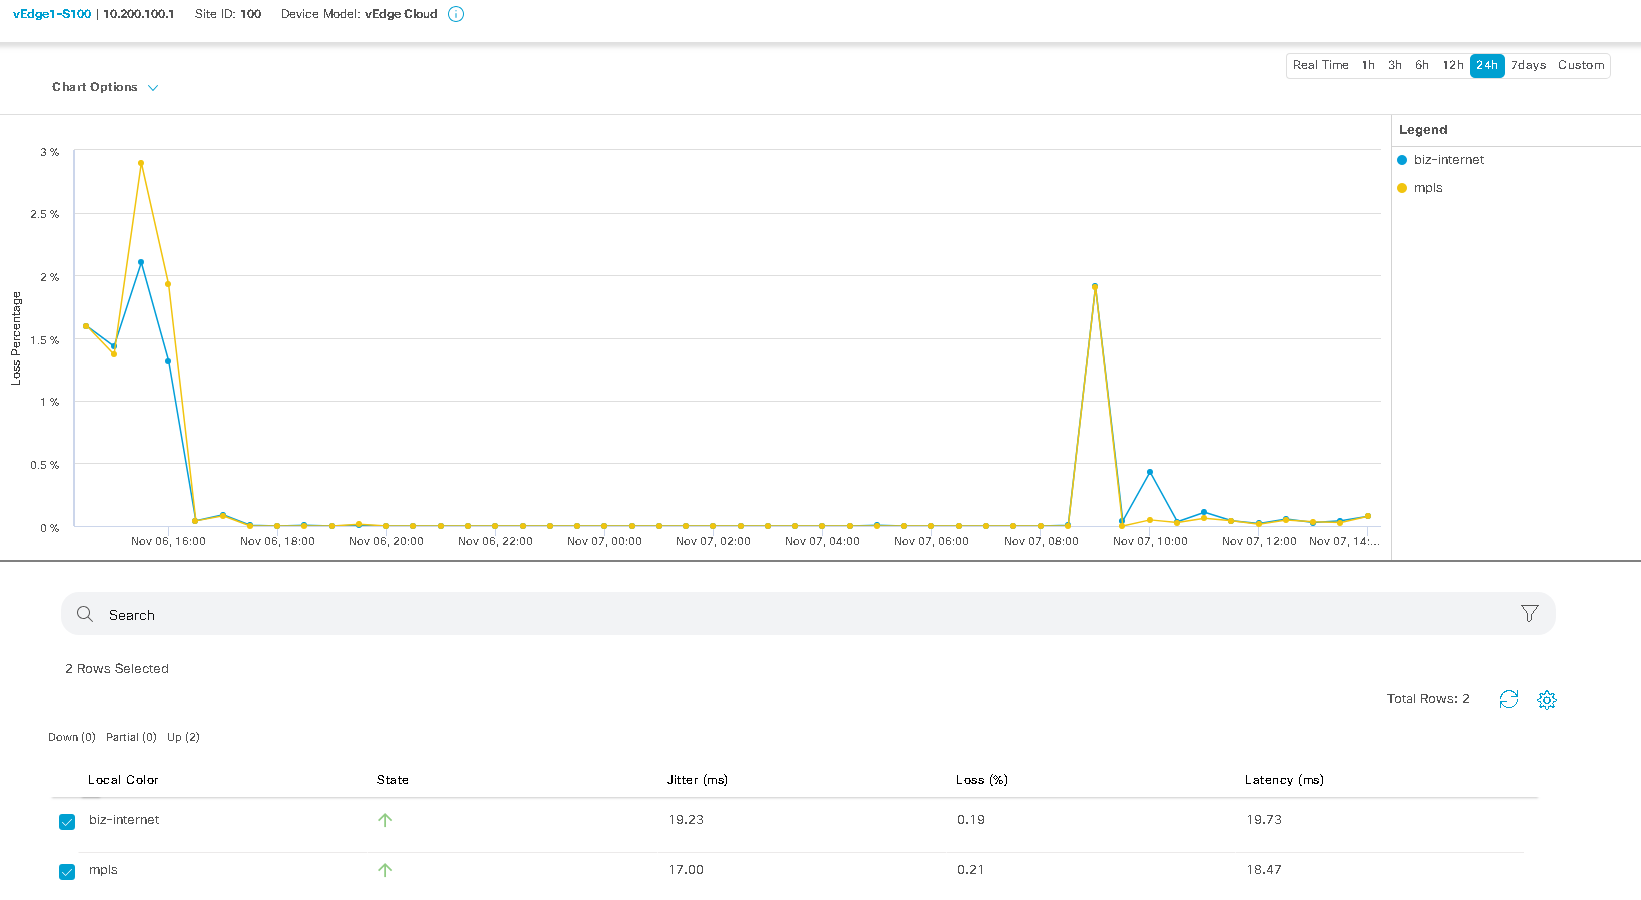
\includegraphics[width=\textwidth]{image/vmanage-tloc-s100-20261107.png}
    \caption{Mất gói theo TLOC của vEdge1-S100 trong 24 giờ, hai color mpls và biz-internet đều up}
    \label{fig:vmanage_tloc}
\end{figure}

\begin{figure}[H]
    \centering
    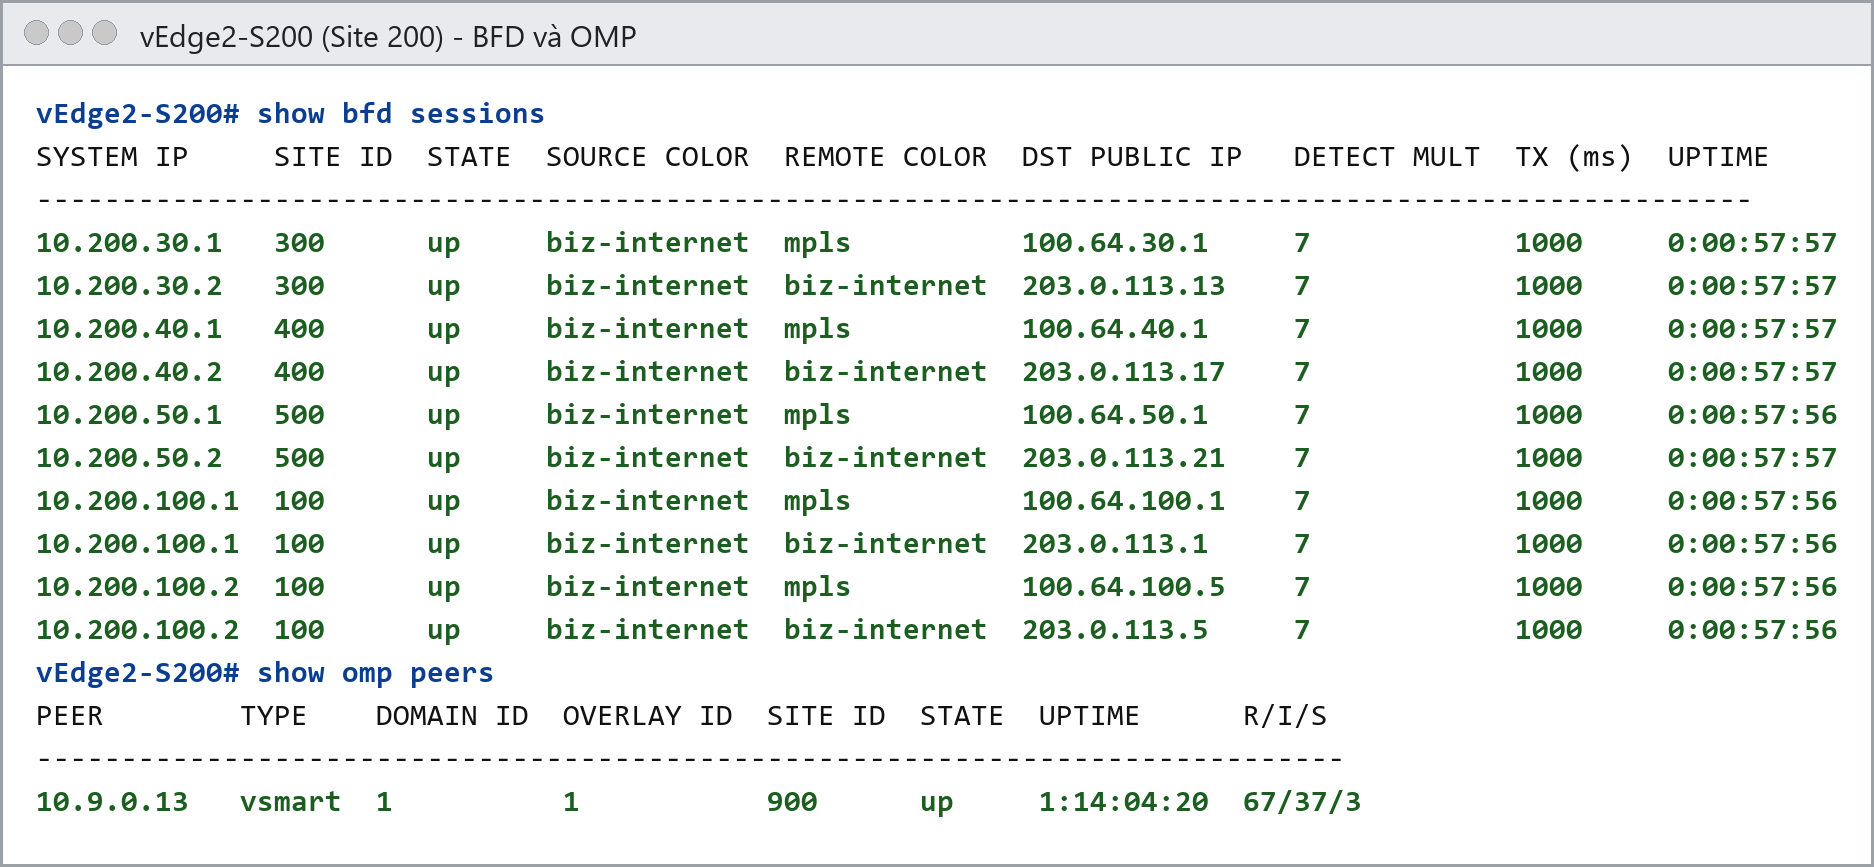
\includegraphics[width=\textwidth]{image/sdwan-bfd-s200.png}
    \caption{vEdge2 Site 200: mười phiên BFD tới các TLOC của Site 100, 300, 400, 500 và phiên OMP với vSmart}
    \label{fig:bfd_s200}
\end{figure}

\begin{table}[H]
    \centering
    \scriptsize
    \caption{Kết quả kiểm thử chính sách tập trung (bộ đếm ghi theo máy trạm Site 200)}
    \label{tab:kiem_thu_chinh_sach}
    \begin{tabularx}{\textwidth}{|c|P{4.3cm}|P{3.9cm}|Z|c|}
        \hline
        \textbf{Mã} & \textbf{Phép thử} & \textbf{Bộ đếm} & \textbf{Thay đổi quan sát} & \textbf{Kết quả} \\
        \hline
        W-1 & vBond có đủ danh sách vEdge hợp lệ & -- & Không thiếu serial & Đạt \\
        \hline
        DP-1 & TCP 23 đến Server Farm bị chặn & TELNET\_TO\_FARM & +9 gói tại vEdge1-S200 & Đạt \\
        \hline
        DP-2 & TCP 22 đến DMZ bị chặn & ADMIN\_TO\_DMZ & +9 gói tại vEdge1-S200 & Đạt \\
        \hline
        DP-3 & HTTP đến DMZ được đi qua & ADMIN\_TO\_DMZ, TELNET\_TO\_FARM, AAR\_WEB & +0, +0 và +17 (được phân loại SLA\_\allowbreak BUSINESS) & Đạt \\
        \hline
        DP-4 & ICMP đến Server Farm được đếm & ICMP\_BRANCH & +15 & Đạt \\
        \hline
        AAR-1 & ICMP liên site theo SLA\_REALTIME & AAR\_ICMP & +54 tại vEdge1-S100, +28 tại vEdge1-S200 & Đạt \\
        \hline
        CP-1 & Chi nhánh chọn vEdge1-S100 cho 10.1.90.0/24 & Bảng tuyến OMP & Tuyến của vEdge1 có cờ C (được chọn), của vEdge2 chỉ có R, xem trên cả vEdge1-S200 và vEdge2-S200 & Đạt \\
        \hline
    \end{tabularx}
\end{table}

Bảng~\ref{tab:kiem_thu_chinh_sach} gồm 7 mã phép thử nhưng ứng với 10 lần kiểm tra: DP-3 kiểm tra đồng thời ba bộ đếm, còn CP-1 được xem trên hai vEdge của Site 200. Công cụ dùng lệnh \texttt{ping -P 6 -p <cổng>} của VPCS để gửi gói TCP SYN đến cổng đích, tương đương một lần mở kết nối Telnet/SSH đối với vEdge. Các bộ đếm tăng đúng như mong đợi đồng thời tại vEdge chi nhánh, chứng minh chính sách chỉ khai báo một lần trên vSmart đã được đẩy xuống và thực thi tại các Edge. Giới hạn của phép thử: luồng kiểm thử xuất phát từ Site 200 và chỉ có một luồng ICMP; việc thực thi chính sách được chứng minh qua bộ đếm trên vEdge, còn khả năng truy cập đầu--cuối vào dịch vụ Campus chính được kiểm chứng riêng ở Mục~\ref{sec:bai_hoc_dich_vu} và các phần kiểm thử dịch vụ.

Các chính sách được cấu hình bằng CLI trực tiếp trên vSmart, không qua giao diện vManage, nên trang Configuration $\rightarrow$ Policies của vManage hiển thị trống; bằng chứng chính sách đang chạy nằm ở đầu ra lệnh trên thiết bị. Khối lệnh~\ref{lst:vsmart_policy_ch4} cho thấy nơi áp chính sách trên vSmart, Khối lệnh~\ref{lst:vedge_policy_ch4} cho thấy vEdge1-S200 đã nhận SLA class, data policy và AAR từ vSmart. \texttt{PREFER-VE1} không có trong đầu ra của vEdge vì control policy được vSmart thực thi khi gửi tuyến OMP, không đẩy xuống Edge.

\begin{lstlisting}[style=customcode,caption={vSmart: show running-config apply-policy},label={lst:vsmart_policy_ch4}]
apply-policy
 site-list ALL_EDGES
  control-policy PREFER-VE1 out
  app-route-policy AAR_LAN
 !
 site-list BRANCHES
  data-policy DP_BRANCH from-service
 !
!
\end{lstlisting}

\begin{lstlisting}[style=customcode,caption={Trích show policy from-vsmart trên vEdge1-S200},label={lst:vedge_policy_ch4}]
from-vsmart sla-class SLA_REALTIME
 loss    2
 latency 150
 jitter  50
from-vsmart data-policy DP_BRANCH
 direction from-service
 vpn-list VPN_LAN
  sequence 10
   match
    destination-data-prefix-list SERVER_FARM
    destination-port             23
    protocol                     6
   action drop
    count TELNET_TO_FARM
from-vsmart app-route-policy AAR_LAN
 vpn-list VPN_LAN
  sequence 10
   match
    protocol 1
   action
    count AAR_ICMP
    sla-class             SLA_REALTIME
    sla-class fallback-to-best-path
\end{lstlisting}

\subsubsection{Báo cáo tình trạng SD-WAN 7 ngày từ vManage}

Ngoài các phép đo tại một thời điểm, dashboard vManage có chức năng xuất báo cáo tổng hợp (\textit{Executive Summary Report}) dạng PDF, gồm ba phần Site, Device và Tunnel. Mỗi phần có trạng thái Good/Fair/Poor hiện tại và biểu đồ theo khung 6 giờ. Bản xuất bao phủ 7 ngày gần nhất tính đến lúc xuất. Tại thời điểm xuất, cả 5 site, 10 vEdge và 112 đường hầm đều ở mức Good. Bảng~\ref{tab:bao_cao_7_ngay} tổng hợp diễn biến theo thời gian, nhãn giờ lấy theo báo cáo.

\begin{table}[H]
    \centering
    \small
    \caption{Diễn biến 7 ngày trong báo cáo vManage (đếm từ biểu đồ; đường hầm là 50 đường kém nhất)}
    \label{tab:bao_cao_7_ngay}
    \begin{tabularx}{\textwidth}{|P{3.5cm}|P{2.6cm}|P{2.6cm}|Z|}
        \hline
        \textbf{Khung thời gian} & \textbf{5 site} & \textbf{10 vEdge} & \textbf{50 đường hầm} \\
        \hline
        31/10 12h -- 01/11 06h & 5 Good & 10 Good & 50 Good; riêng 01/11 06h: 21 Good, 29 Fair \\
        \hline
        01/11 12h & 4 Fair, 1 Good & 8 Fair, 2 Good & 10 Poor, 7 Fair, 33 Good \\
        \hline
        01/11 18h & 4 Fair, 1 Good & 8 Fair, 1 Good, 1 không có dữ liệu & 10 Poor, 35 Good, 5 không có dữ liệu \\
        \hline
        02/11 00h & 5 Good & 10 Good & 50 Good \\
        \hline
        02/11 06h & 5 Good & 10 Good & 50 Fair \\
        \hline
        02/11 12h -- 18h & Không có dữ liệu & Không có dữ liệu & 50 Poor \\
        \hline
        03/11 00h -- 06/11 06h & Không có dữ liệu & Không có dữ liệu & Không có dữ liệu (hệ thống ngừng vận hành) \\
        \hline
        06/11 12h & 5 Good & 10 Good & 26 Good, 24 Fair \\
        \hline
        06/11 18h -- 07/11 12h & 5 Good & 10 Good & 50 Good \\
        \hline
    \end{tabularx}
\end{table}

Từ báo cáo có thể rút ra các nhận định sau:

\begin{itemize}
    \item \textbf{Giai đoạn 01--02/11} khớp với nhật ký vận hành: tường lửa FW-ASAv Site 100 khởi động lại lặp do \texttt{route track} và \texttt{sla monitor}, đã sửa ngày 02/11. Site 500 vẫn Good trong khi bốn site còn lại xuống Fair (Hình~\ref{fig:bc7_site}). Mười đường hầm Poor ngày 01/11 đều tới \texttt{vEdge1-S500:mpls} (Hình~\ref{fig:bc7_tunnel}), phù hợp với việc vEdge1-S500 unreachable từ tối 01/11 (Hình~\ref{fig:bc7_thietbi}).
    \item \textbf{Giai đoạn 03--06/11} không có dữ liệu vì hệ thống được ngừng vận hành có chủ đích trong giai đoạn này, không phải sự cố; dữ liệu có lại khi vManage khởi động chiều 06/11 (cột Up Since ở Hình~\ref{fig:vmanage_devices}). Báo cáo của vManage chỉ phản ánh các khung thời gian hệ thống đang chạy. Cả 50 đường hầm Poor ở hai khung 02/11 12h--18h, ngay trước khoảng này, nhiều khả năng ứng với quá trình dừng hệ thống; nhận định này chưa được kiểm chứng.
    \item \textbf{Nhãn Good không đồng nghĩa không mất gói.} Trong mục đường hầm Good ở khung hiện tại, năm đường có mất gói cao nhất đều đi qua TLOC biz-internet của vEdge2-S200, mất 15,5--15,6\% so với gần 0\% ở 12 giờ trước, độ trễ tới 72,57~ms (Hình~\ref{fig:bc7_chiso}). Nhật ký trên vEdge giải thích con số này. Khoảng 17 phút trước khi xuất báo cáo, các vEdge Site 100 và Site 200 cùng mất kết nối điều khiển tới cả ba controller do hết thời gian chờ (\texttt{VS\_TMO}, \texttt{VM\_TMO}, \texttt{VB\_TMO}); toàn bộ phiên BFD của vEdge2-S200 rớt và dựng lại trong khoảng 3 giây với cổng nguồn mới. Hiện tượng tương tự đã xảy ra khoảng 5 giờ trước đó. Đọc lại vào sáng hôm sau, cả mười đường hầm của vEdge2-S200 mất 0--1 gói trên khoảng 120 gói thăm dò mỗi cửa sổ. Như vậy mức 15,6\% phản ánh sự kiện ngắn nằm trong khung tính, không phải mất gói kéo dài. Vì sao controller hết thời gian chờ đồng loạt thì chưa xác định.
\end{itemize}

\begin{figure}[H]
    \centering
    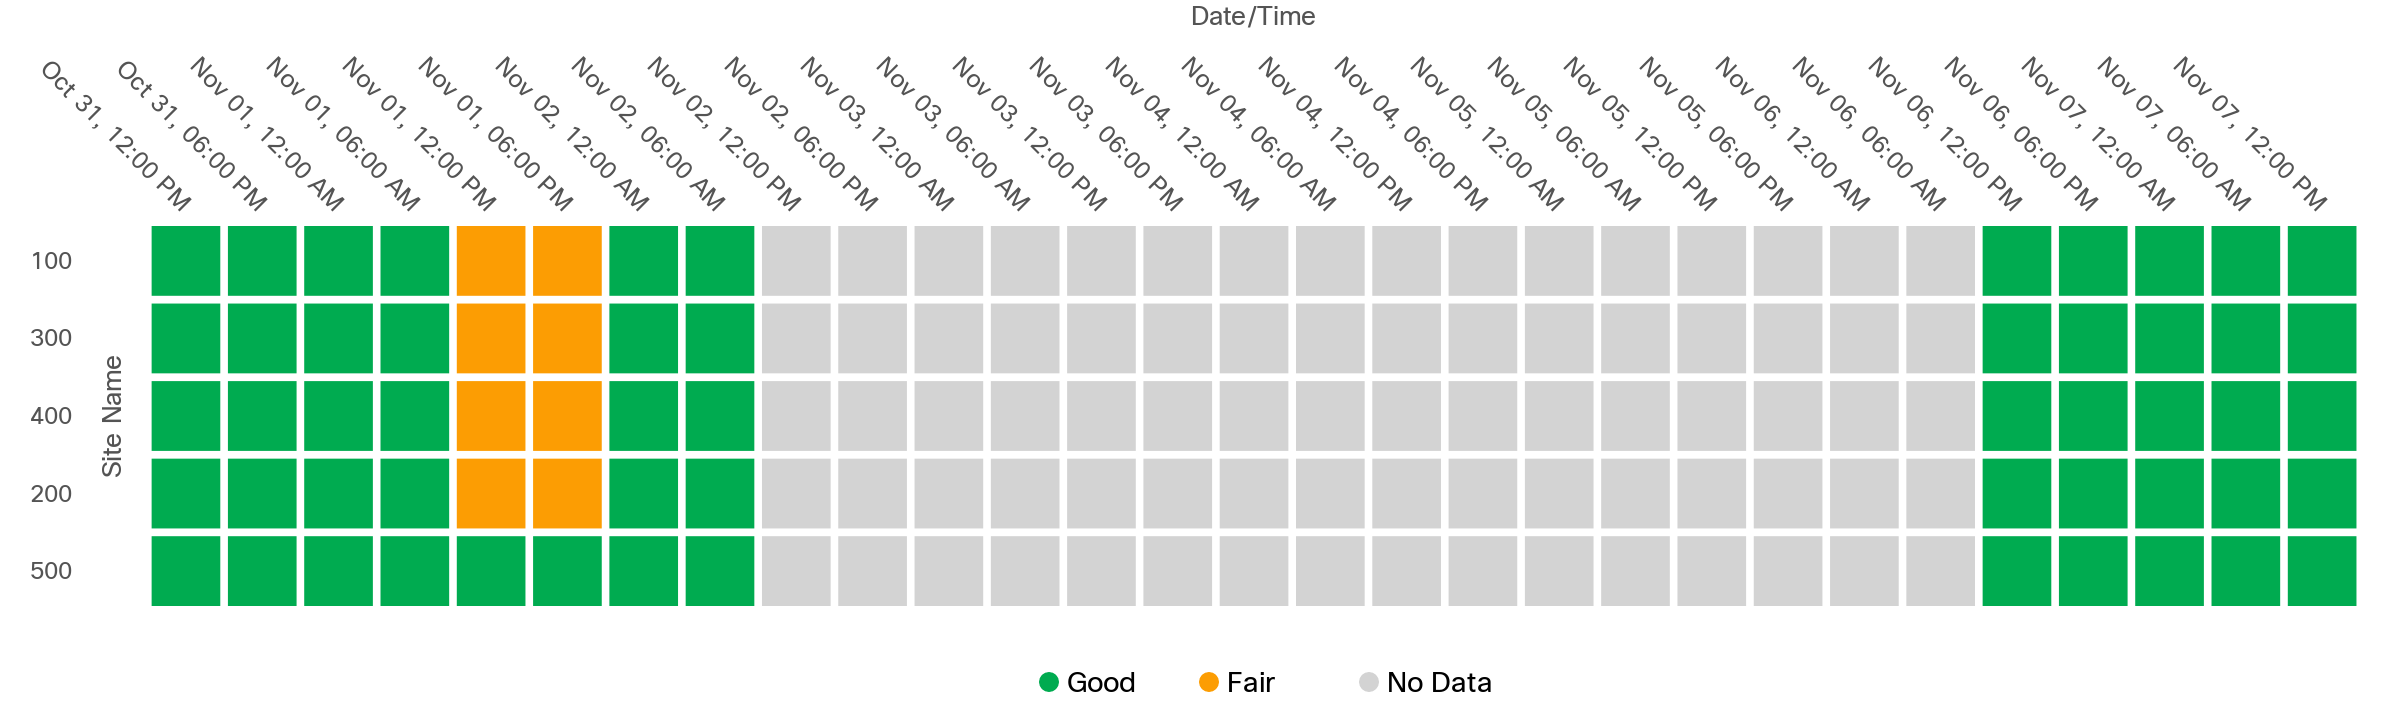
\includegraphics[width=\textwidth]{image/vmanage-7ngay-site.png}
    \caption{Báo cáo vManage: tình trạng 5 site theo khung 6 giờ trong 7 ngày}
    \label{fig:bc7_site}
\end{figure}

\begin{figure}[H]
    \centering
    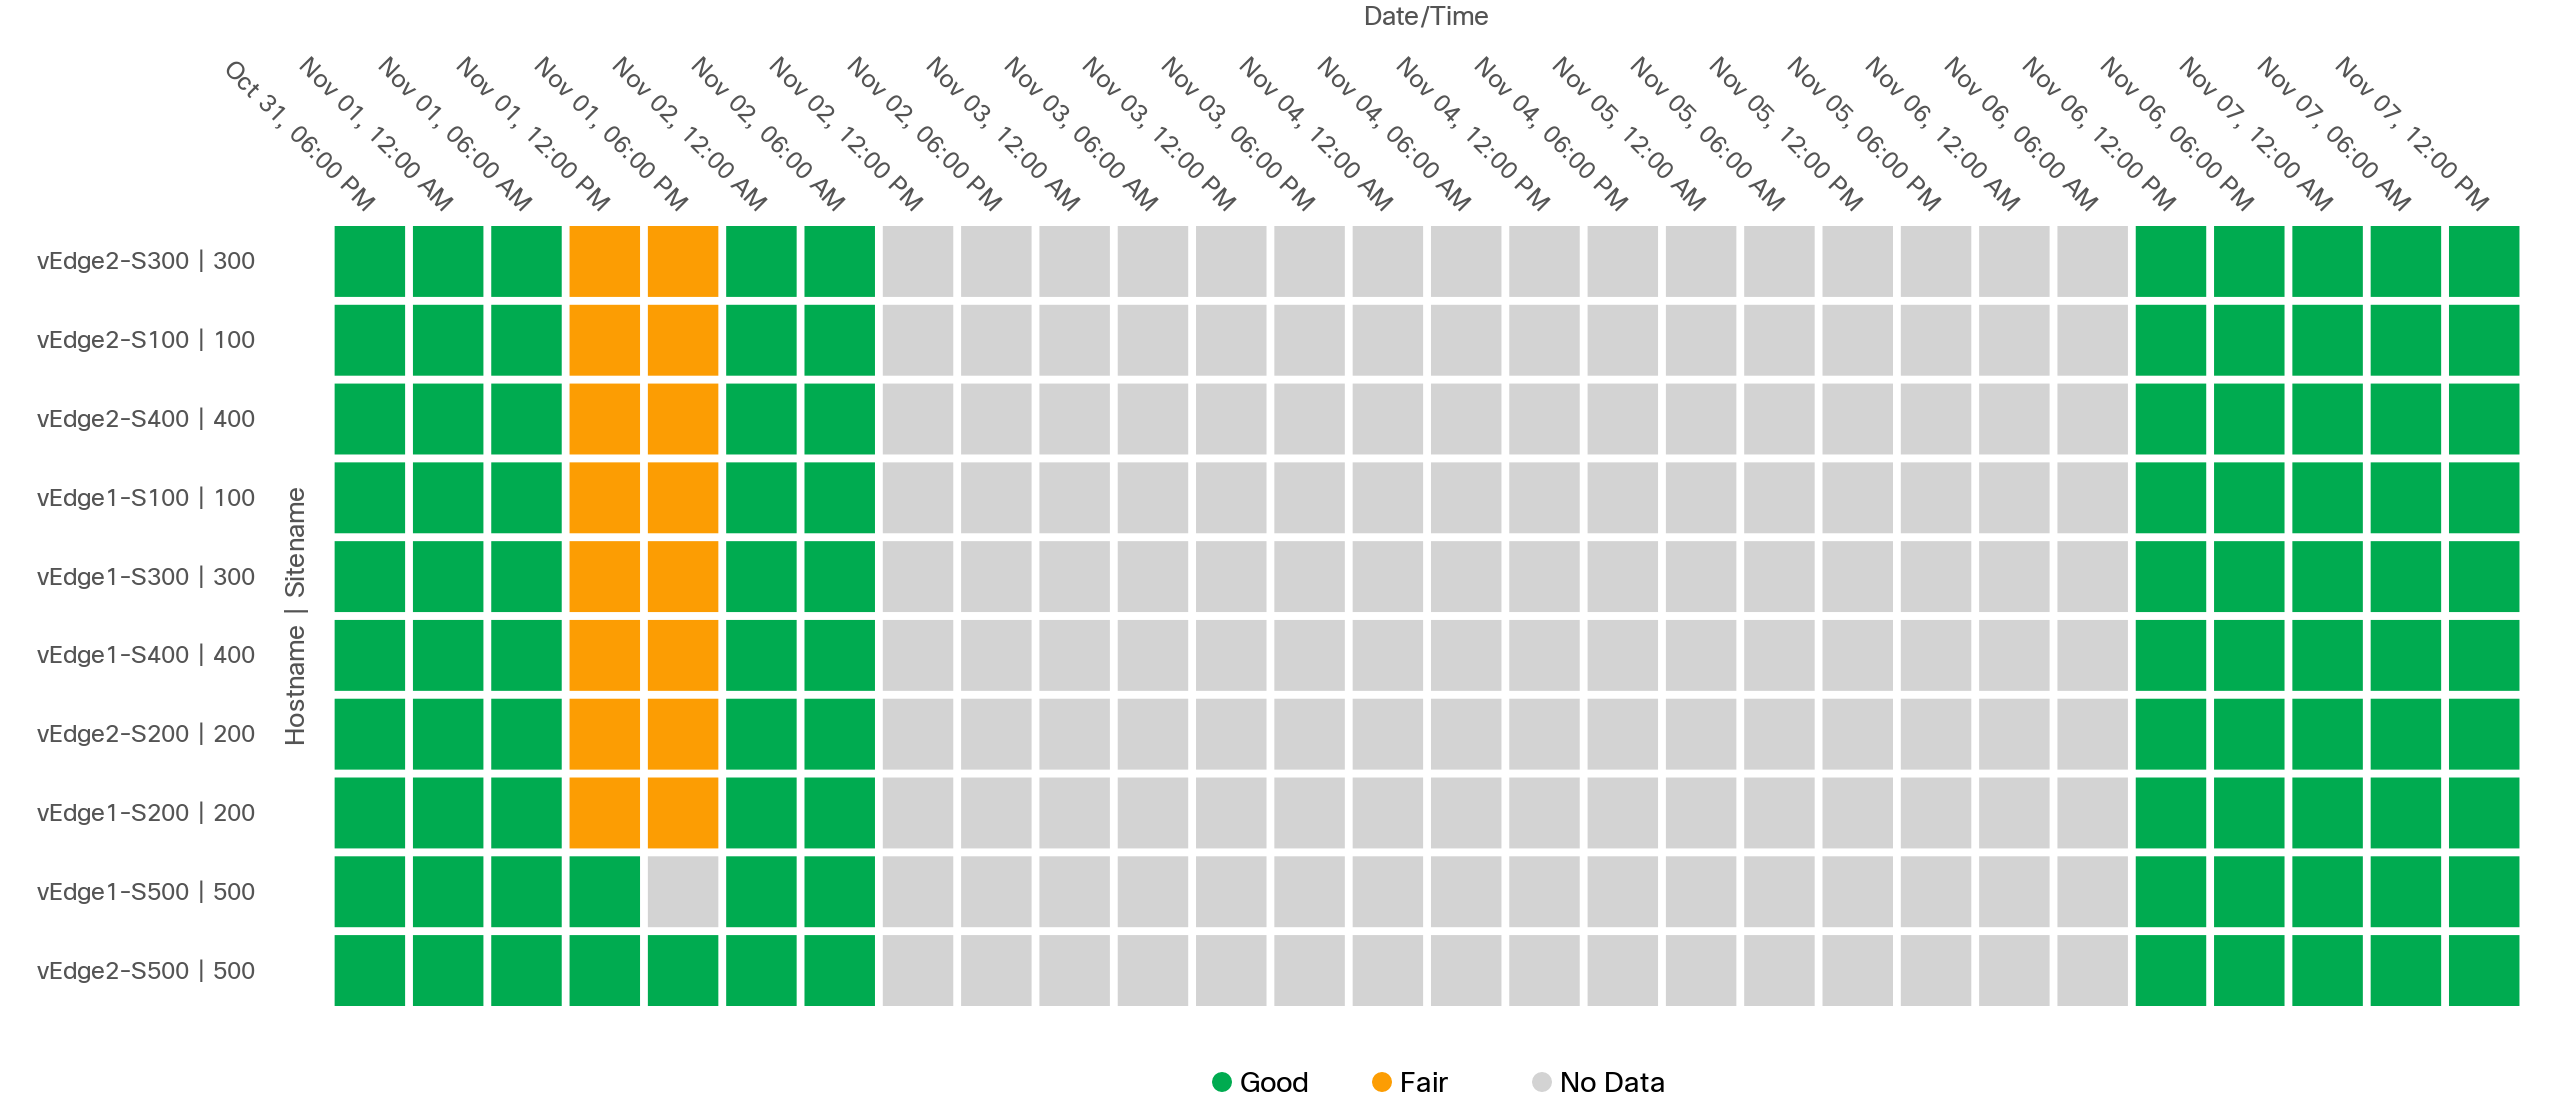
\includegraphics[width=\textwidth]{image/vmanage-7ngay-thietbi.png}
    \caption{Báo cáo vManage: tình trạng 10 vEdge theo khung 6 giờ}
    \label{fig:bc7_thietbi}
\end{figure}

\begin{figure}[H]
    \centering
    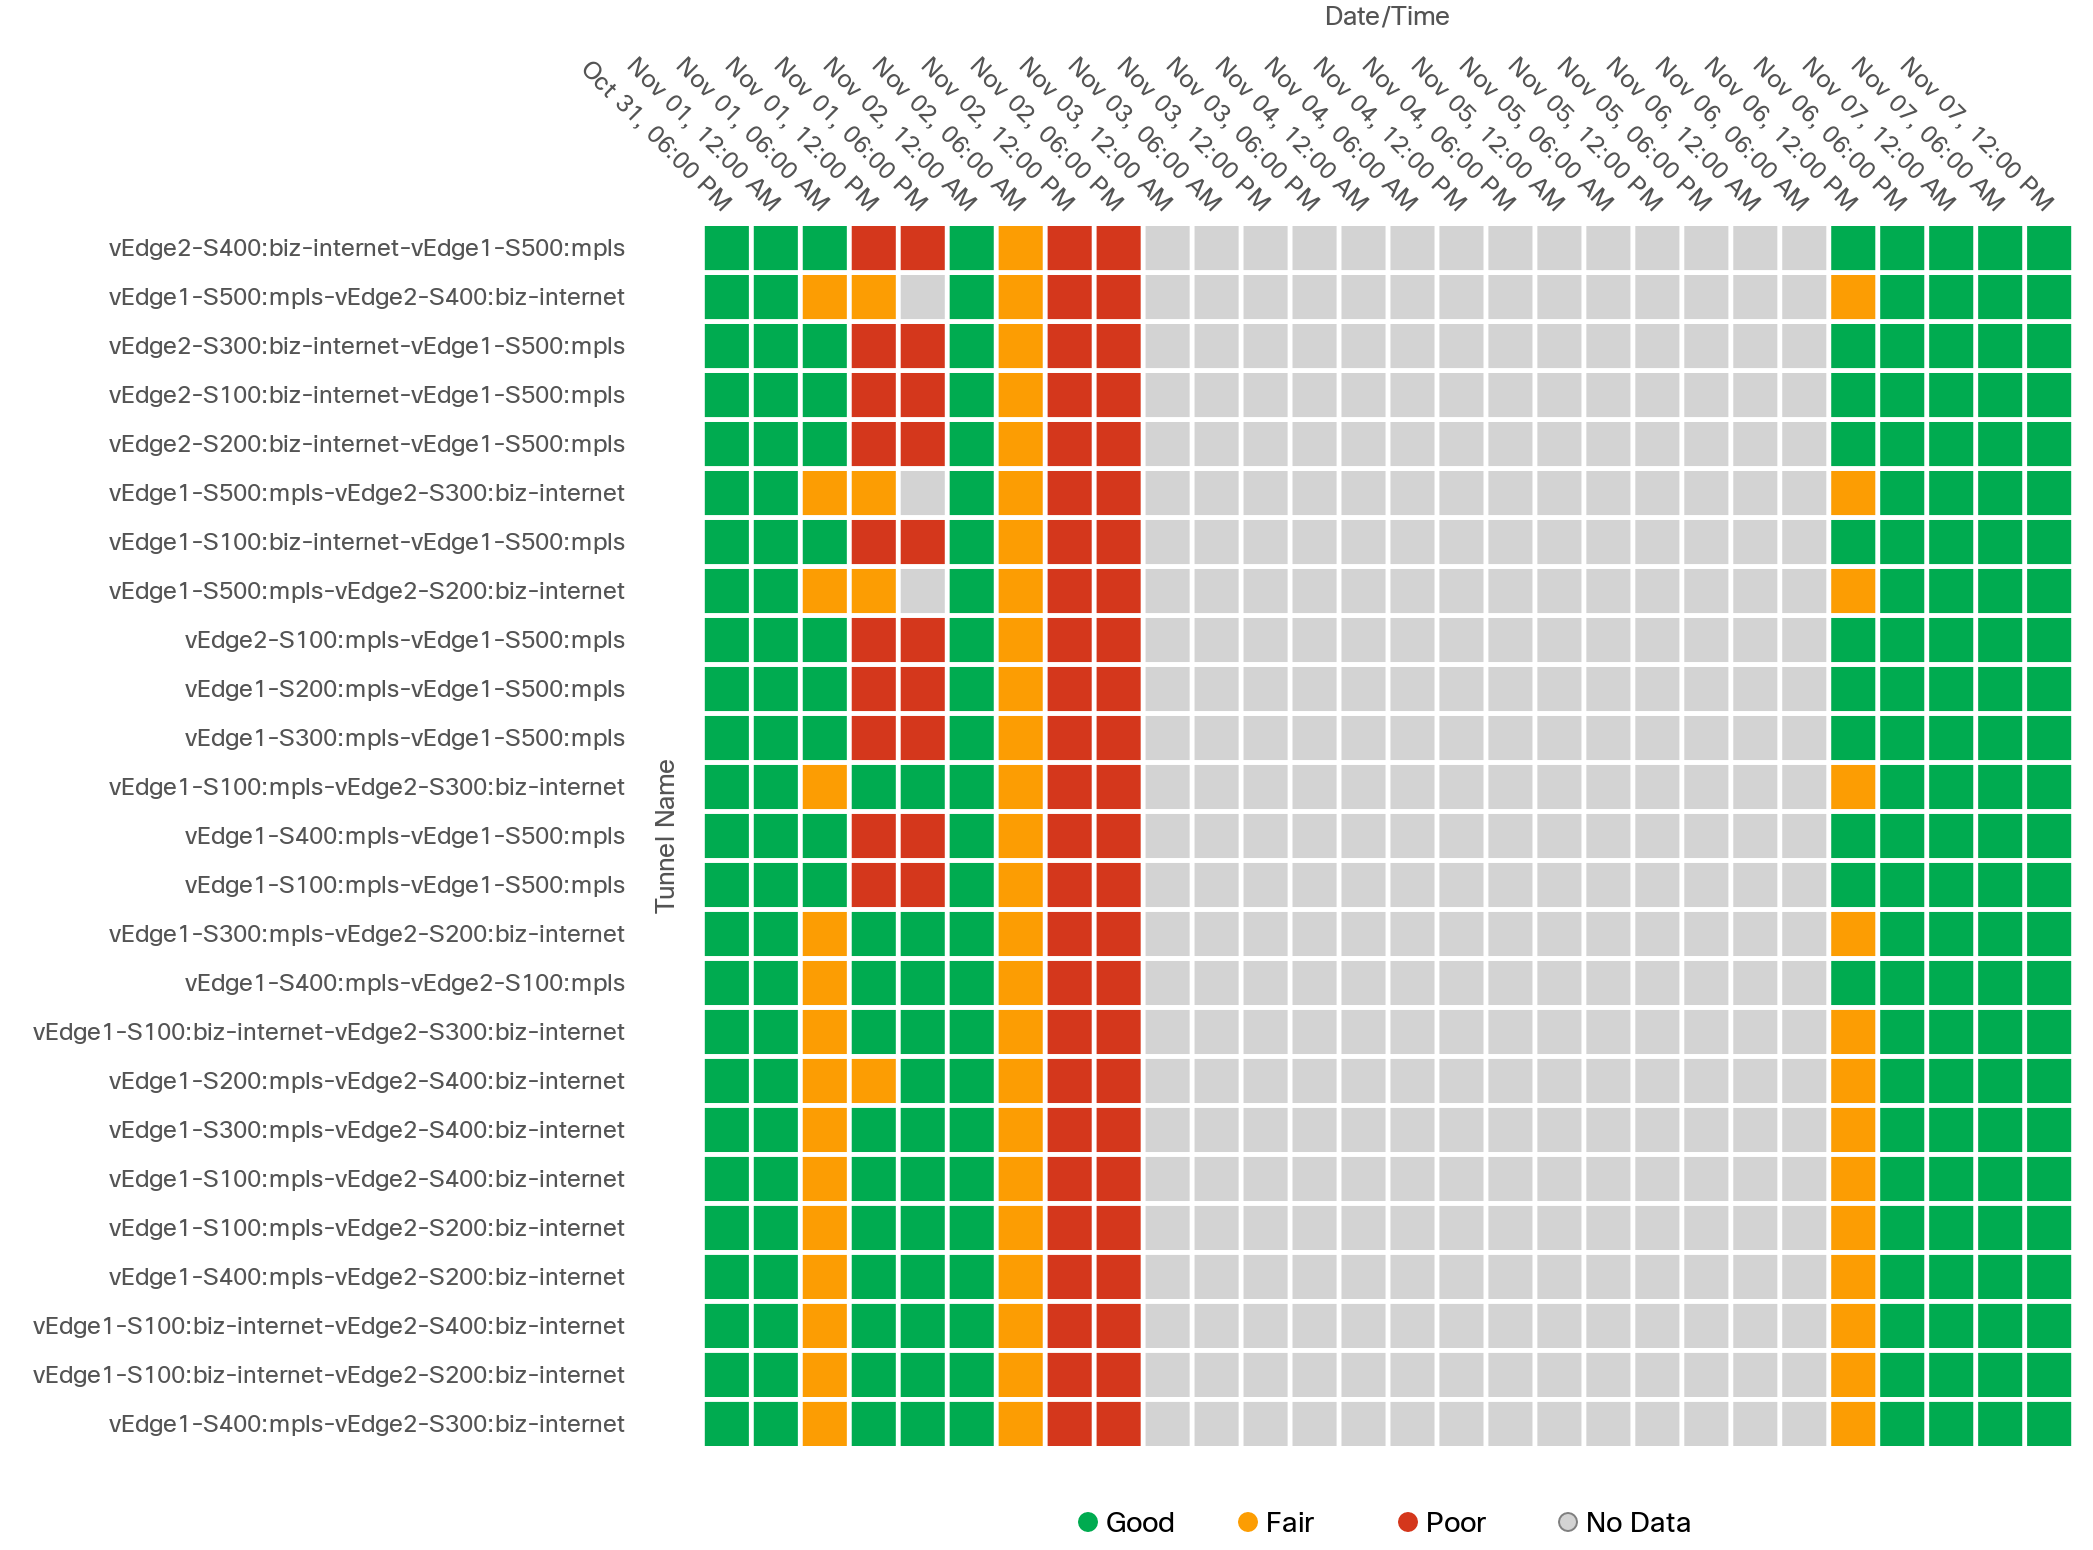
\includegraphics[width=0.9\textwidth]{image/vmanage-7ngay-tunnel.png}
    \caption{Báo cáo vManage: 25 trong 50 đường hầm kém nhất theo khung 6 giờ}
    \label{fig:bc7_tunnel}
\end{figure}

\begin{figure}[H]
    \centering
    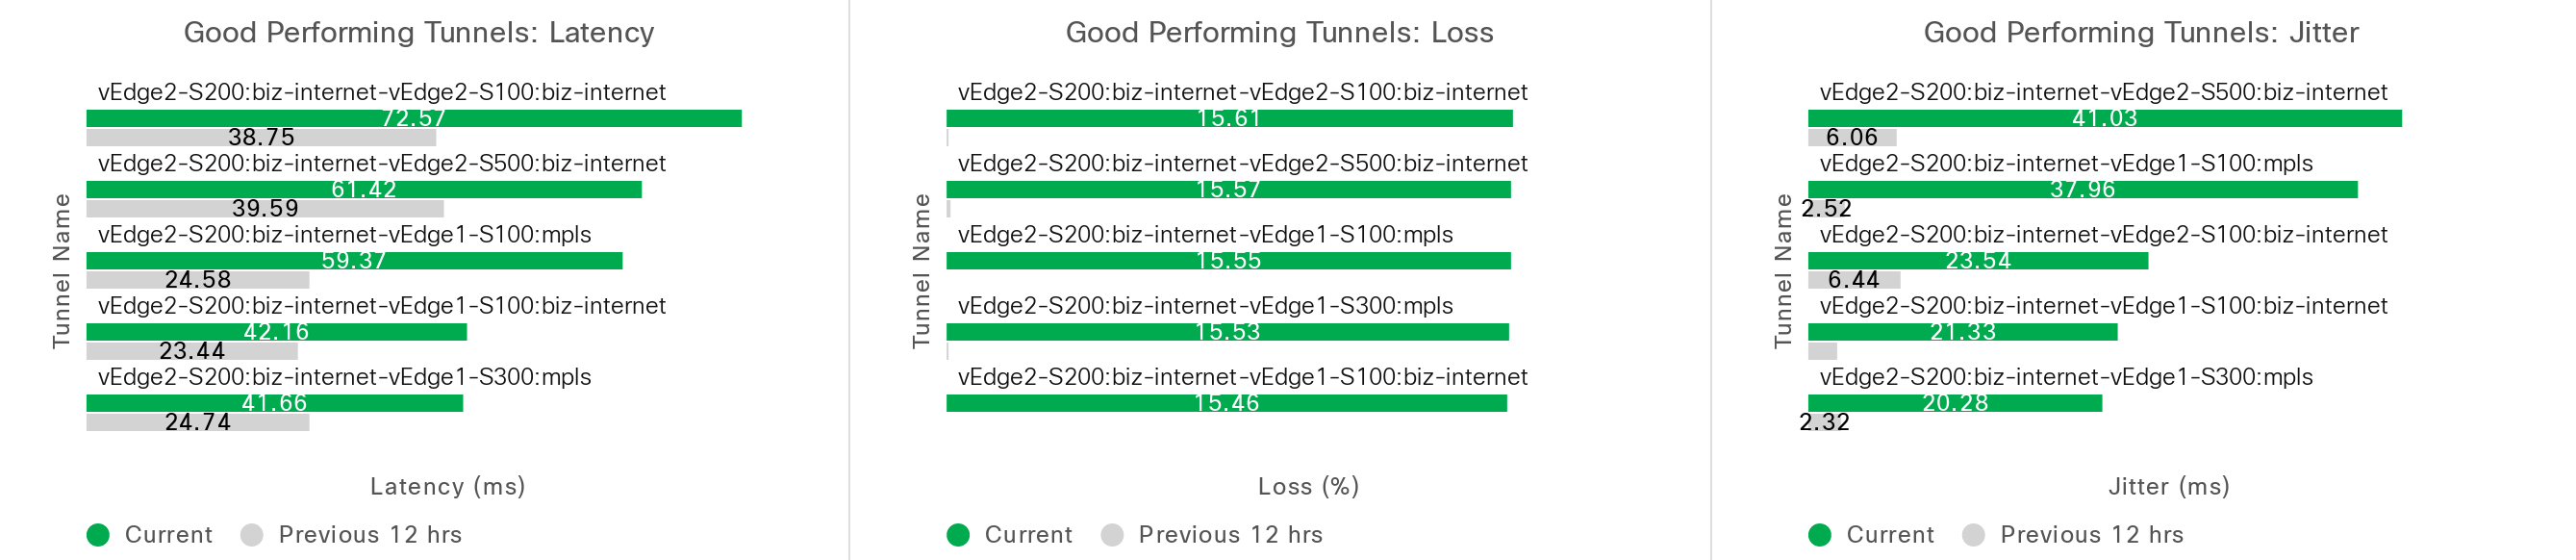
\includegraphics[width=\textwidth]{image/vmanage-7ngay-tunnel-chiso.png}
    \caption{Báo cáo vManage: năm đường hầm cao nhất theo độ trễ, mất gói và jitter trong nhóm Good, so với 12 giờ trước}
    \label{fig:bc7_chiso}
\end{figure}

\subsection{Truy cập Internet và cảnh báo sự cố}

\subsubsection{Triển khai}

Việc cho người dùng ra Internet được làm theo từng giai đoạn, kiểm thử xong giai đoạn trước mới sang giai đoạn sau: (1) router Internet nhận địa chỉ DHCP từ mạng thật của phòng lab, PAT các dải \texttt{203.0.113.0/24} và \texttt{100.64.0.0/10}; (2) vEdge Site 100 bật \texttt{nat} trên cổng \texttt{biz-internet} và thêm tuyến mặc định kiểu NAT trong VPN 1; (3) chi nhánh: vEdge2 tương tự, Brand-FW tách tuyến nội bộ và tuyến Internet (Khối lệnh~\ref{lst:brandfw_ch4}); (4) DNS Server chuyển tiếp tên ngoài, tường lửa biên chỉ cho riêng máy chủ DNS hỏi ra ngoài; (5) chính sách theo vùng (VLAN 99, Server Farm, DMZ, Site 900); (6) ma trận kiểm thử. Dự phòng Internet của chi nhánh được thực hiện bằng NAT trên cổng MPLS của vEdge1 kèm IP SLA \texttt{track 2} trên Brand-FW.

Cảnh báo email được triển khai sau cùng: Switch32 mở thêm một dòng ACL cho riêng vManage gửi SMTP 587, vManage được khai báo DNS (\texttt{vpn 0 dns 8.8.8.8 primary}), sau đó cấu hình máy chủ SMTP và luật thông báo \texttt{SDWAN-DOWN-ALERT} trên giao diện vManage.

\subsubsection{Các vấn đề kỹ thuật}\label{sec:bai_hoc_internet}

\begingroup
\small
\begin{longtable}{|L{3.0cm}|L{5.2cm}|L{5.3cm}|}
    \caption{Các vấn đề khi triển khai Internet và cảnh báo}\label{tab:loi_internet} \\
    \hline
    \textbf{Hiện tượng} & \textbf{Nguyên nhân gốc} & \textbf{Khắc phục} \\
    \hline
    \endfirsthead
    \hline
    \textbf{Hiện tượng} & \textbf{Nguyên nhân gốc} & \textbf{Khắc phục} \\
    \hline
    \endhead
    \hline
    \endfoot
    Router Internet mất Internet ngay sau khi bật NAT trên vEdge Site 100 & Phiên BGP lên lại, vEdge quảng bá ngược tuyến mặc định học từ MPLS; eBGP (AD 20) thắng tuyến mặc định DHCP (AD 254), tạo vòng lặp & Prefix-list \texttt{NO\_DEFAULT\_IN} chiều vào trên mọi láng giềng của router Internet, làm mới bằng \texttt{clear ip bgp * soft in} (không reset phiên) \\
    \hline
    Lưu lượng Internet chia tải sang MPLS và bị mất & VPN 0 có hai tuyến mặc định ECMP, MPLS ban đầu không có đường ra Internet & Router Internet gửi tuyến mặc định cho router MPLS và NAT cả dải \texttt{100.64.0.0/10} \\
    \hline
    Tuyến mặc định của chi nhánh xuất hiện ở mọi site & Tuyến tĩnh mặc định trong VPN 1 của vEdge1 bị \texttt{advertise static} quảng bá vào OMP & Chỉ dùng tuyến mặc định kiểu NAT (không lên OMP); để Brand-FW chọn đường ra \\
    \hline
    Khi vEdge2 hỏng, máy trạm vẫn không tới được một số đích Internet & Đích thăm dò SLA ban đầu là \texttt{8.8.8.8}; tuyến \texttt{/32} ghim gói thăm dò kéo cả lưu lượng người dùng tới \texttt{8.8.8.8} về vEdge2 đã hỏng & Đổi đích thăm dò sang \texttt{9.9.9.9} \\
    \hline
    Ping từ VLAN 99 Campus chính tới chi nhánh thất bại & Tường lửa biên có giao diện management nối trực tiếp \texttt{10.1.99.0/24} nên gói trả về đi ra management, không khớp phiên trên inside (bất đối xứng) & \texttt{management-only} cho Management0/0 và tuyến \texttt{10.1.99.0/24} qua Core-SW1 \\
    \hline
    vManage không gửi được thư cảnh báo & Máy chủ SMTP từ chối xác thực (\texttt{535 Username and Password not accepted}) do thông tin nhập trên giao diện sai; mạng không chặn (bộ đếm ACL của luồng 587 vẫn tăng) & Nhập lại tài khoản đầy đủ và mật khẩu ứng dụng; xác nhận qua nhật ký gửi thư của vManage \\
\end{longtable}
\endgroup

\subsubsection{Kết quả kiểm thử}

\begin{table}[H]
    \centering
    \small
    \caption{Ma trận kiểm thử truy cập Internet}
    \label{tab:kiem_thu_internet}
    \begin{tabularx}{\textwidth}{|L{5.6cm}|Y|}
        \hline
        \textbf{Kiểm thử} & \textbf{Kết quả} \\
        \hline
        Máy trạm Site 200/300/400: DHCP và \texttt{ping google.com} & Đạt, 3/3 mỗi site; DNS \texttt{10.1.90.10}, tên miền \texttt{campus.internal} \\
        \hline
        Tên nội bộ \texttt{www.campus.internal} sau khi bật chuyển tiếp DNS & Đạt, vẫn phân giải \texttt{10.1.1.10} \\
        \hline
        Traceroute từ chi nhánh ra Internet & Đạt, chặng đầu là vEdge2 tại chỗ (DIA), không vòng qua Site 100 \\
        \hline
        Cắt \texttt{biz-internet} tại Site 200, rồi khôi phục & Đạt: \texttt{track 2} Down sau khoảng 30 giây, Internet chuyển sang MPLS (ping \texttt{8.8.8.8}, \texttt{google.com} 3/3); khôi phục thì quay về vEdge2 \\
        \hline
        Site 100: VLAN 10 ra Internet / VLAN 99 ra Internet & Đạt: 3/3 / bị chặn đúng thiết kế \\
        \hline
        VLAN 99 Campus chính tới chi nhánh & Đạt: 10/10 tới Site 200, 5/5 tới Site 300, Site 400 \\
        \hline
        Site 900 ra Internet có kiểm soát & Đạt: DNS, HTTPS, ping qua; HTTP 80, SSH 22 bị chặn; kết nối điều khiển của fabric không bị ảnh hưởng \\
        \hline
    \end{tabularx}
\end{table}

\begin{figure}[H]
    \centering
    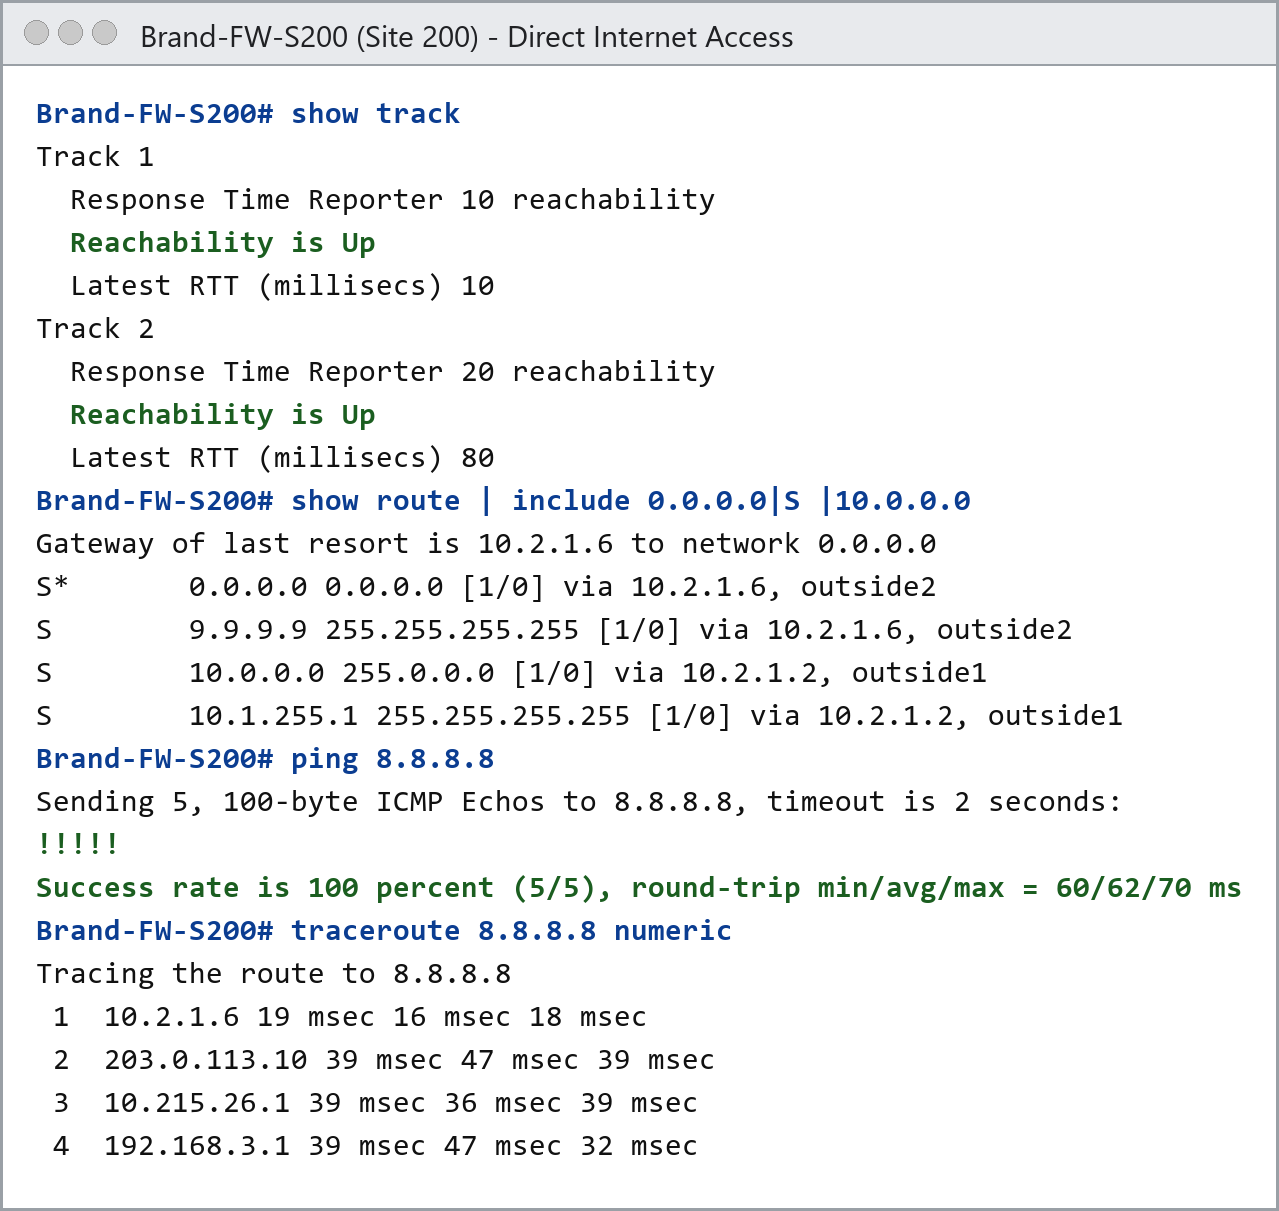
\includegraphics[width=0.75\textwidth]{image/dia-brandfw-s200.png}
    \caption{Brand-FW Site 200: hai đối tượng track, tuyến mặc định qua vEdge2 và traceroute ra Internet}
    \label{fig:dia_brandfw}
\end{figure}

\textbf{Cảnh báo email:} khi tắt cổng \texttt{biz-internet} của vEdge2 Site 200, vManage gửi thư cảnh báo cho từng sự kiện (Bảng~\ref{tab:canh_bao_email}); khi bật lại cổng, thiết bị phục hồi đủ 3 kết nối điều khiển và 8 phiên BFD, vManage gửi thư cho sự kiện Interface State Change. Luật thông báo chọn mức Critical, Major và Medium cùng các alarm phục hồi BFD, Control, OMP Up, nên quản trị viên nhận cả thư báo lỗi lẫn thư báo phục hồi.

\begin{table}[H]
    \centering
    \small
    \caption{Thư cảnh báo khi tắt và bật lại cổng Internet của vEdge2 Site 200}
    \label{tab:canh_bao_email}
    \begin{tabularx}{\textwidth}{|P{3.2cm}|Z|P{2.4cm}|}
        \hline
        \textbf{Thời điểm sau khi tắt cổng} & \textbf{Sự kiện} & \textbf{Thư} \\
        \hline
        khoảng 20 giây & All BFD sessions for the node are down & Đã gửi \\
        \hline
        khoảng 35 giây & All Control connections for the node are down & Đã gửi \\
        \hline
        khoảng 70 giây & All OMP sessions for the node are down & Đã gửi \\
        \hline
        khi bật lại cổng & Interface State Change & Đã gửi \\
        \hline
    \end{tabularx}
\end{table}

\subsection{Triển khai dịch vụ}

\subsubsection{DHCP và DNS}

DHCP Server tại \texttt{10.1.90.10} chạy vai trò DHCP của Windows Server 2012 R2 với bốn scope đang hoạt động cho VLAN 10--40; mỗi scope có dải \texttt{.100--.199}, gateway \texttt{.1}, DNS \texttt{10.1.90.10} (option 6) và tên miền \texttt{campus.internal} (option 15). Relay từ hai Core có \texttt{giaddr} tương ứng \texttt{.2} và \texttt{.3} nên máy chủ chọn đúng scope. Cùng máy chủ chạy DNS với zone thuận \texttt{campus.internal} (bản ghi A cho www, web, mail, dns, dhcp, syslog; bản ghi MX trỏ mail), zone ngược cho DMZ và chuyển tiếp tên ngoài tới \texttt{8.8.8.8}, \texttt{1.1.1.1} (tắt root hints). Hình~\ref{fig:dhcp_scopes} và Hình~\ref{fig:dhcp_leases} là giao diện quản trị DHCP: bốn scope đều \texttt{Active} và scope VLAN 10 đang cấp hai lease cho máy trạm của Campus chính; Hình~\ref{fig:dns_zone} là zone \texttt{campus.internal} với bản ghi MX và các bản ghi A của dịch vụ.

\begin{figure}[H]
    \centering
    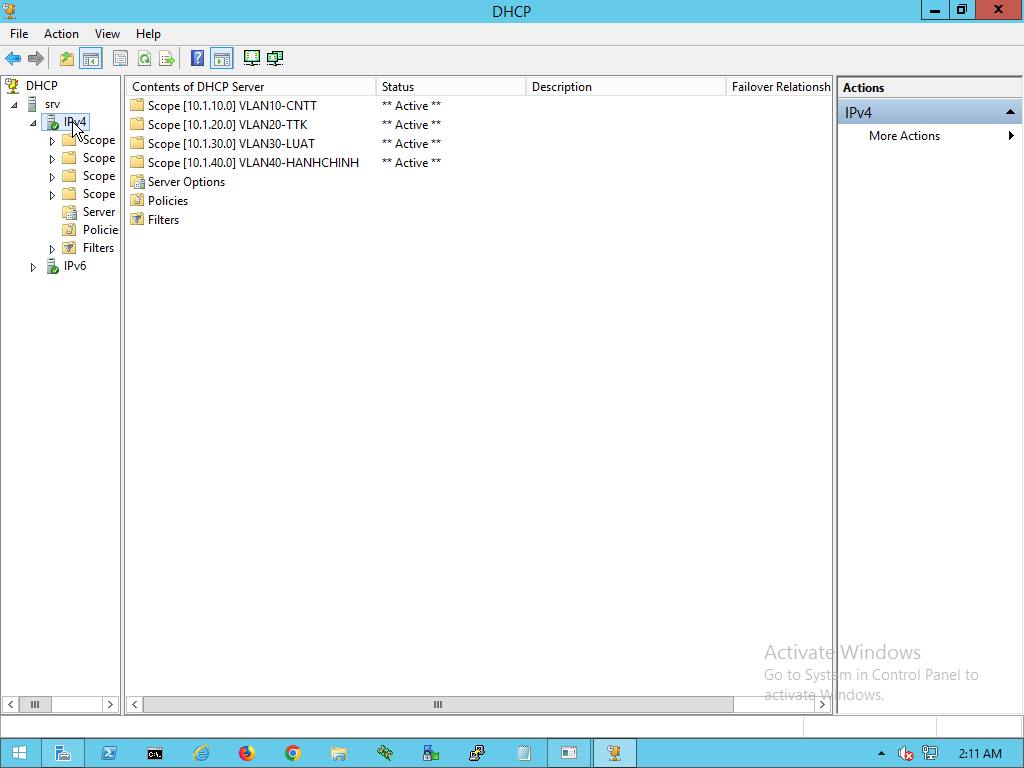
\includegraphics[width=0.8\textwidth]{image/dhcp-scopes-20261108.png}
    \caption{DHCP Server (Windows Server 2012 R2): bốn scope VLAN 10--40 đang hoạt động}
    \label{fig:dhcp_scopes}
\end{figure}

\begin{figure}[H]
    \centering
    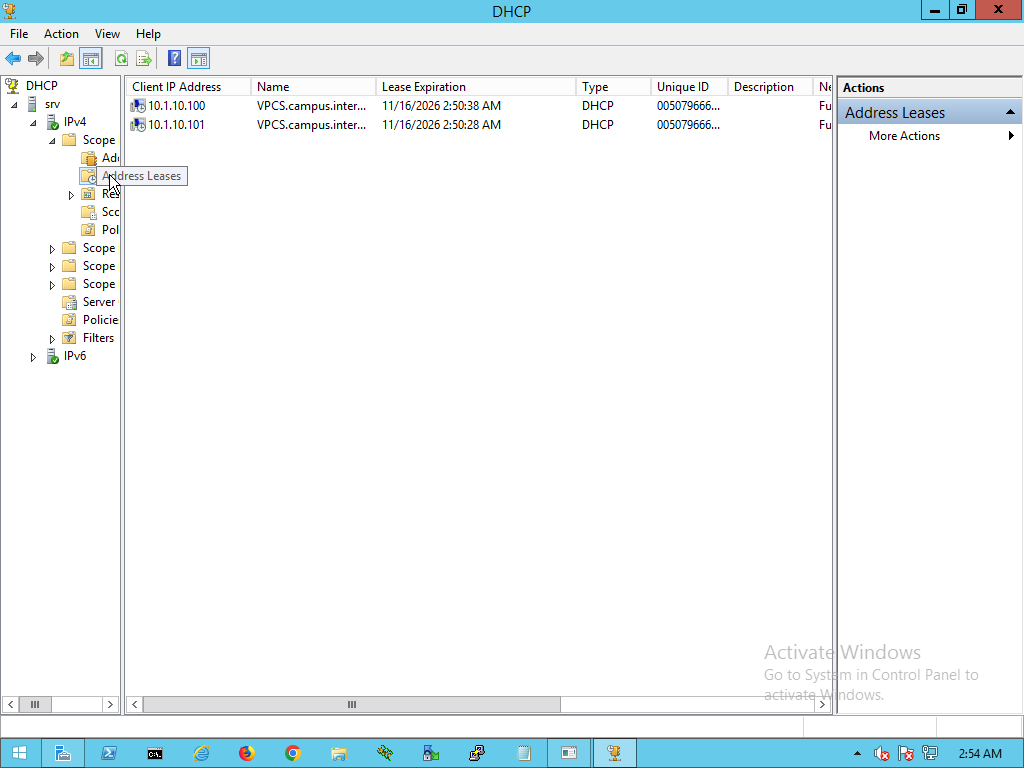
\includegraphics[width=0.8\textwidth]{image/dhcp-leases-vlan10-20261108.png}
    \caption{Lease đã cấp trong scope VLAN 10 qua DHCP Relay của Core}
    \label{fig:dhcp_leases}
\end{figure}

\begin{figure}[H]
    \centering
    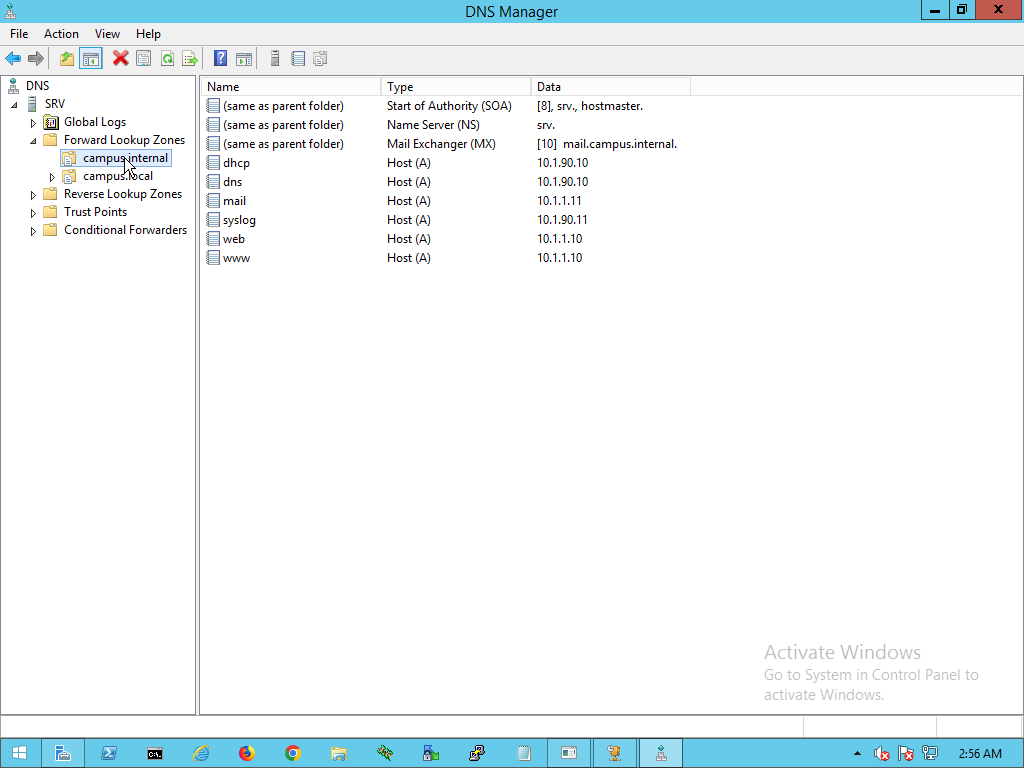
\includegraphics[width=0.8\textwidth]{image/dns-zone-20261108.png}
    \caption[DNS Manager: zone campus.internal và các bản ghi dịch vụ]{DNS Manager: zone \texttt{campus.internal} với bản ghi MX và bản ghi A cho dhcp, dns, mail, syslog, web, www}
    \label{fig:dns_zone}
\end{figure}

\subsubsection{Web và Mail}

Web Server chạy Nginx với chứng chỉ tự ký cho \texttt{www.campus.internal} (SAN gồm tên web và địa chỉ \texttt{10.1.1.10}); HTTP được chuyển hướng 301 sang HTTPS; trang \texttt{/whoami} trả về địa chỉ máy khách để kiểm chứng đường đi. Mail Server chạy hMailServer 5.6.8 với tên miền \texttt{campus.internal}, năm hộp thư (\texttt{admin}, \texttt{hanhchinh}, \texttt{luhanh}, \texttt{taichinh}, \texttt{yte}; Hình~\ref{fig:hmail_accounts}), mở các cổng 25, 110, 143, 587 trên tường lửa của máy chủ.

\begin{figure}[H]
    \centering
    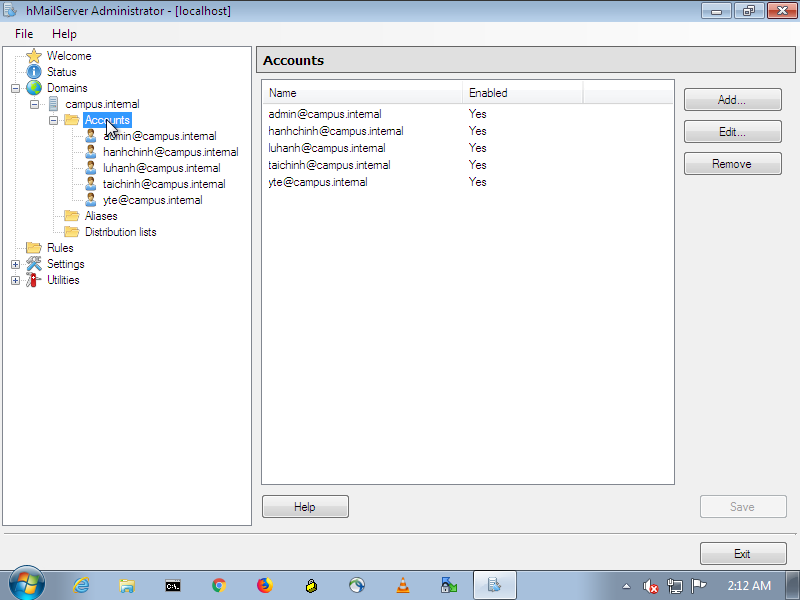
\includegraphics[width=0.75\textwidth]{image/mail-hmail-accounts-20261108.png}
    \caption[hMailServer Administrator: tên miền và năm hộp thư]{hMailServer Administrator: tên miền \texttt{campus.internal} và năm hộp thư}
    \label{fig:hmail_accounts}
\end{figure}

\subsubsection{Các vấn đề kỹ thuật tại lớp dịch vụ}\label{sec:bai_hoc_dich_vu}

\textbf{Tên miền \texttt{.local}:} ban đầu hệ thống dùng \texttt{campus.local}. Máy trạm Ubuntu phân giải được bằng \texttt{dig} nhưng trình duyệt và ứng dụng thư không tìm thấy máy chủ, vì cấu hình phân giải tên mặc định chuyển \texttt{*.local} cho mDNS và trả ``không tồn tại'' trước khi hỏi DNS. Hệ thống được chuyển sang \texttt{campus.internal}: tạo zone mới, đổi option 15 trên DHCP Server và \texttt{dhcpd domain} trên ba Brand-FW, cấp lại chứng chỉ Web, đổi tên miền trên Mail Server (giữ \texttt{campus.local} làm bí danh trong giai đoạn chuyển tiếp). Sau khi chuyển, máy trạm Ubuntu với cấu hình mặc định phân giải đúng mọi tên nội bộ.

\textbf{Giới hạn bảng kết nối của tường lửa:} ASAv chạy không có giấy phép chỉ cho phép tối đa 100 kết nối đồng thời. Khi lab chưa có Internet, các truy vấn DNS ra ngoài không có lời đáp chiếm đầy bảng kết nối, khiến kết nối IMAP từ chi nhánh bị từ chối dù ping vẫn thành công. Nguyên nhân được xác định qua bộ đếm \texttt{Denied} của \texttt{show resource usage} và công cụ \texttt{packet-tracer}. Khắc phục bằng ACL \texttt{INSIDE\_OUT} chỉ cho máy chủ DNS hỏi ra ngoài và giảm thời gian chờ của phiên DNS xuống 10 giây; số kết nối giảm từ 100 xuống khoảng 45 và ổn định. Sau khi có Internet, bảng kết nối khi kiểm thử chỉ khoảng 7/100. Giới hạn băng thông của ASAv không giấy phép vẫn đủ cho ping và phân giải tên nhưng không đủ để duyệt web thực tế.

\subsubsection{Kết quả kiểm thử dịch vụ}

Phép thử được thực hiện từ máy trạm Ubuntu PC-YTe-S200 (\texttt{10.2.70.103}) tại chi nhánh Cần Thơ, qua overlay SD-WAN và tường lửa biên:
\begin{itemize}
    \item DHCP cấp \texttt{search campus.internal}; tên \texttt{www}, \texttt{mail} và bản ghi MX phân giải đúng.
    \item \texttt{https://www.campus.internal/whoami} trả về \texttt{client=10.2.70.103}, chứng minh gói đi thẳng từ chi nhánh qua overlay không bị NAT; chứng chỉ đúng tên; HTTP được chuyển hướng sang HTTPS; cổng không được công bố (8080) bị tường lửa chặn.
    \item Gửi thư qua SMTP 587 có xác thực từ hộp thư \texttt{yte} đến hộp thư \texttt{admin} của tên miền \texttt{campus.internal} thành công; đọc thư qua IMAP; tiêu đề \texttt{Received} ghi nhận địa chỉ \texttt{10.2.70.103}.
    \item Ứng dụng thư trên máy trạm Ubuntu ở ba chi nhánh kết nối IMAP ổn định sau khi xử lý giới hạn bảng kết nối.
\end{itemize}

\textbf{Kiểm thử từ Campus chính.} Máy trạm Ubuntu tại VLAN 40 (PC-HanhChinh-S100, địa chỉ \texttt{10.1.40.102}) truy cập dịch vụ qua mạng SDN, Core và tường lửa biên vào DMZ: máy kết nối được TCP 143 và 587 tới Mail Server \texttt{10.1.1.11}; Firefox mở được trang \texttt{https://www.campus.internal} và trang \texttt{/whoami} trả về \texttt{client=10.1.40.102} (Hình~\ref{fig:web_s100}, Hình~\ref{fig:whoami_s100}); Thunderbird gửi thành công thư từ hộp thư \texttt{hanhchinh} tới \texttt{yte} qua SMTP 587 (Hình~\ref{fig:mail_s100}).

\begin{figure}[H]
    \centering
    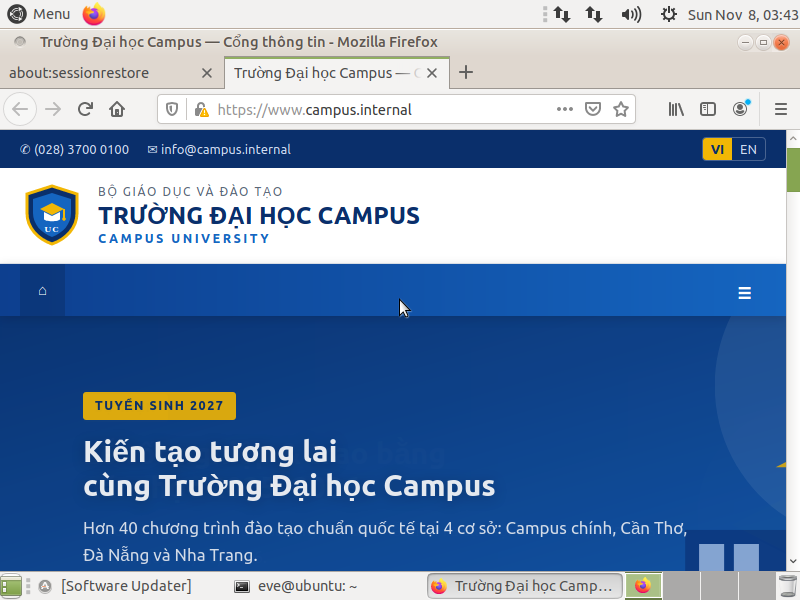
\includegraphics[width=0.8\textwidth]{image/web-campus-s100-20261108.png}
    \caption[Trang web của trường mở từ máy trạm VLAN 40 Campus chính]{Trang web \texttt{https://www.campus.internal} mở từ PC-HanhChinh-S100 tại VLAN 40 Campus chính}
    \label{fig:web_s100}
\end{figure}

\begin{figure}[H]
    \centering
    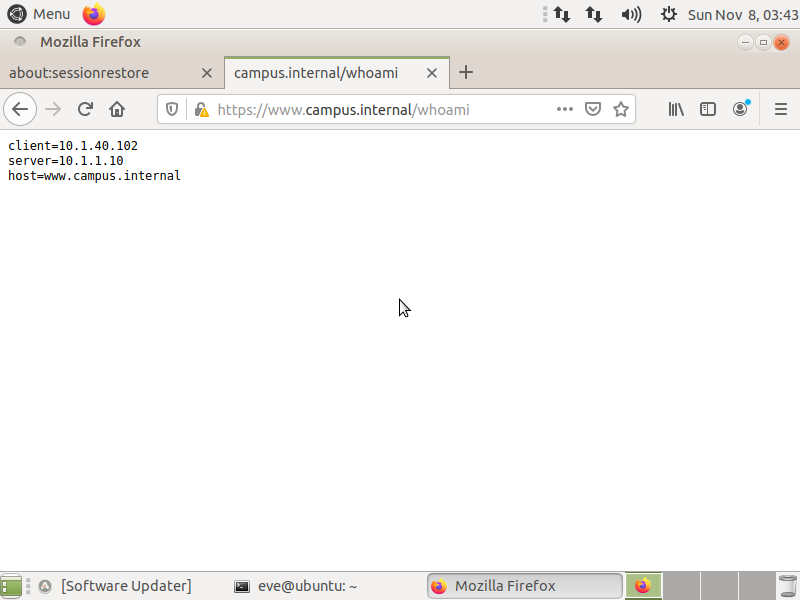
\includegraphics[width=0.8\textwidth]{image/web-whoami-s100-20261108.png}
    \caption[Trang whoami: máy chủ Web thấy đúng địa chỉ máy trạm]{Trang \texttt{/whoami}: máy chủ Web thấy đúng địa chỉ máy trạm \texttt{10.1.40.102}, không qua NAT}
    \label{fig:whoami_s100}
\end{figure}

\begin{figure}[H]
    \centering
    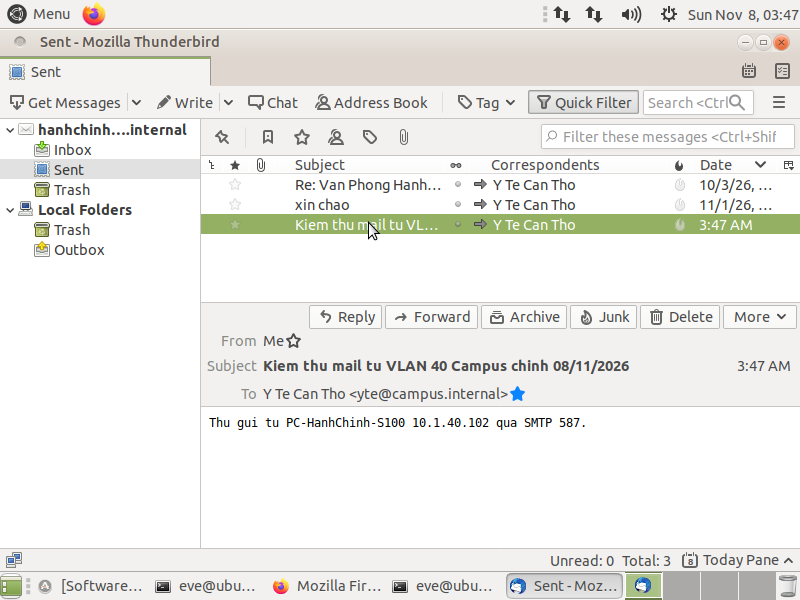
\includegraphics[width=0.8\textwidth]{image/mail-sent-s100-20261108.png}
    \caption[Thunderbird trên PC-HanhChinh-S100: thư kiểm thử gửi qua SMTP 587]{Thunderbird trên PC-HanhChinh-S100: thư kiểm thử gửi từ \texttt{hanhchinh@campus.internal} tới \texttt{yte@campus.internal} qua SMTP 587}
    \label{fig:mail_s100}
\end{figure}

Syslog Server (Kiwi Syslog, \texttt{10.1.90.11}) nhận nhật ký thực tế từ tường lửa và các thiết bị hạ tầng qua UDP 514; tường lửa Active ghi nhật ký ở mức \texttt{informational} và bộ đếm \texttt{Trap logging} của nó cho thấy hơn 11.000 bản tin đã được gửi tới máy chủ này. Hình~\ref{fig:syslog_kiwi} là màn hình Kiwi Syslog: nhật ký của Web Server (\texttt{10.1.1.10}) đi qua tường lửa tới cổng UDP 514 của máy chủ, tường lửa ghi lại kết nối này (\texttt{\%ASA-6-302015}) và các gói bị luật \texttt{INSIDE\_OUT} chặn, ví dụ gói DNS từ VLAN 99 ra Internet (\texttt{\%ASA-4-106023}).

\begin{figure}[H]
    \centering
    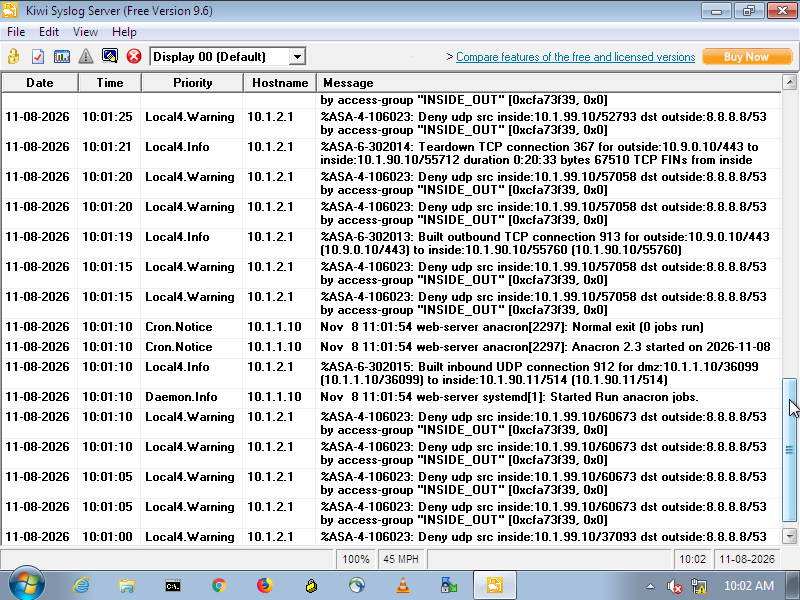
\includegraphics[width=0.85\textwidth]{image/syslog-kiwi-20261108.png}
    \caption{Kiwi Syslog nhận nhật ký từ tường lửa (\texttt{10.1.2.1}) và Web Server (\texttt{10.1.1.10})}
    \label{fig:syslog_kiwi}
\end{figure}

\subsection{Vận hành tự động: Campus NetOps Bot}\label{sec:netops_bot}

Để giảm thao tác thủ công khi giám sát hệ thống nhiều thành phần (Ryu, vManage, tường lửa, hơn bốn mươi thiết bị Cisco/Viptela), nhóm phát triển \textit{Campus NetOps Bot}: một trợ lý vận hành qua Telegram chạy ngay trong topology, trên máy chủ Windows Server tại Server Farm của Campus chính (\texttt{10.1.90.10}). Bot kết nối thiết bị bằng SSH trong băng (in-band) với tài khoản riêng \texttt{netops}, chỉ được phép từ hai địa chỉ quản trị (ACL \texttt{NETOPS\_MGMT} trên vty); với các chi nhánh, bot đi qua overlay SD-WAN. Bot đọc REST API của vManage và của SDN Controller. Chỉ những người dùng Telegram có trong danh sách cho phép mới dùng được bot, và mật khẩu không bao giờ được gửi tới mô hình ngôn ngữ. Các chức năng chính:

\begin{itemize}
    \item \textbf{Hỏi đáp và lệnh chỉ đọc:} người vận hành hỏi bằng ngôn ngữ tự nhiên hoặc dùng lệnh trực tiếp (\texttt{/health}, \texttt{/show}, \texttt{/ping}, \texttt{/dhcp}); bộ lọc chỉ cho phép \texttt{show}, \texttt{ping}, \texttt{traceroute} và che mật khẩu, khóa trong đầu ra.
    \item \textbf{Chẩn đoán theo lớp} (\texttt{/diag}): mỗi bài chẩn đoán dừng ở lớp lỗi đầu tiên và đưa bằng chứng. Với vEdge: cổng transport $\rightarrow$ BGP underlay $\rightarrow$ tuyến mặc định $\rightarrow$ kết nối điều khiển $\rightarrow$ OMP $\rightarrow$ BFD. Với DHCP Campus chính: OVS và liên kết SDN $\rightarrow$ SVI Core $\rightarrow$ relay $\rightarrow$ DHCP Server. Với tường lửa: HA, giao diện, OSPF, tuyến mặc định, gói bị hủy. Ngoài ra có bài cho SDN và cho DHCP từng chi nhánh.
    \item \textbf{Cảnh báo chủ động:} đọc alarm mới của vManage, phát hiện vManage mất kết nối, OVS mất Controller, liên kết OVS chết hoặc Controller khựng lâu; mỗi cảnh báo kèm nút chạy chẩn đoán ngay hoặc tạm tắt một giờ. Cảnh báo vẫn được gửi khi chính vManage hỏng, khắc phục điểm yếu của thư cảnh báo chỉ do vManage gửi; bot có chống báo lặp khi một sự kiện dao động liên tục.
    \item \textbf{Thay đổi cấu hình có duyệt và tự hoàn tác} (\texttt{/change}): bot hiển thị các dòng sẽ thêm, chỉ áp khi người có quyền bấm Duyệt, chụp trạng thái trước/sau (cổng, BGP, OSPF, VRRP, BFD); nếu trạng thái xấu đi thì tự hoàn tác (\texttt{configure replace} trên IOS, \texttt{commit confirmed} trên Viptela). Kiểm tra tuân thủ thiết kế (\texttt{/compliance}), sao lưu và so lệch cấu hình với kho mã (\texttt{/backup}, \texttt{/drift}).
\end{itemize}

Hình~\ref{fig:bot_health} là kết quả lệnh \texttt{/health}: 13/13 thiết bị SD-WAN reachable, đủ phiên BFD, và bốn kiểm tra của SDN Site 100 đều đạt. Hình~\ref{fig:bot_diag_fw} là bài chẩn đoán tường lửa: HA Primary Active/Secondary Standby Ready, 7/7 giao diện up, sáu láng giềng OSPF \texttt{FULL}. Bộ tự kiểm tra của bot (DNS, kết nối Telegram, SSH tới hai tường lửa và các switch Site 100 và chi nhánh, REST của Ryu và vManage) đạt 23/23 mục.

\begin{figure}[H]
    \centering
    \begin{minipage}[t]{0.49\textwidth}
        \centering
        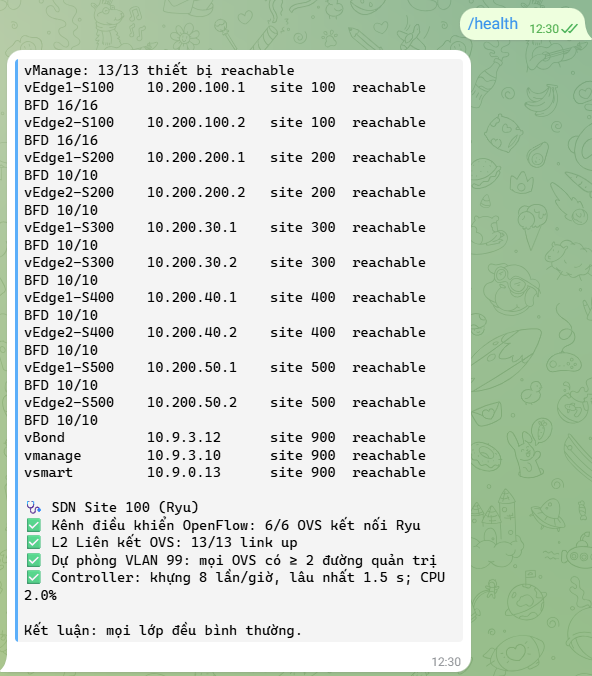
\includegraphics[width=\textwidth]{image/netops-bot-health.png}
        \caption{NetOps Bot: lệnh \texttt{/health} tổng hợp SD-WAN và SDN}
        \label{fig:bot_health}
    \end{minipage}\hfill
    \begin{minipage}[t]{0.49\textwidth}
        \centering
        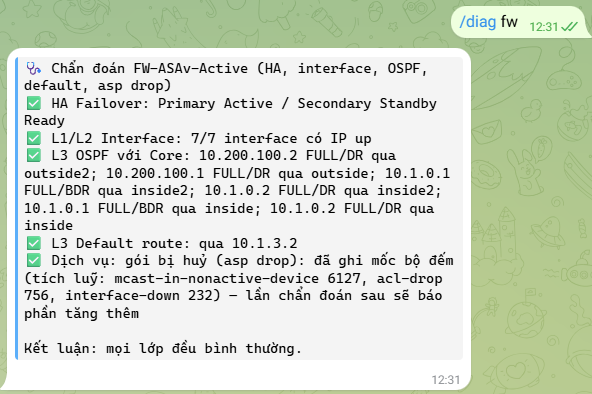
\includegraphics[width=\textwidth]{image/netops-bot-diag-fw.png}
        \caption{NetOps Bot: chẩn đoán theo lớp tường lửa HA Site 100}
        \label{fig:bot_diag_fw}
    \end{minipage}
\end{figure}

Bot đã phát huy tác dụng trong sự cố ngày 01/11/2026: Telegram nhận hàng trăm cảnh báo OSPF và kết nối điều khiển. Từ các cảnh báo này, nhóm xác định được hai vEdge Site 100 rớt OSPF cùng một giây, rồi tìm ra nguyên nhân là cặp tường lửa khởi động lại lặp (Mục~\ref{sec:fw_ha}).

\subsection{Tổng hợp kết quả kiểm thử}

\begingroup
\scriptsize
\setlength{\tabcolsep}{3pt}
\begin{longtable}{|P{0.7cm}|P{2.8cm}|L{3.4cm}|P{1.8cm}|L{4.0cm}|}
    \caption{Tổng hợp kịch bản kiểm thử và kết quả}\label{tab:kiem_thu_tong_hop_ch4} \\
    \hline
    \textbf{Mã} & \textbf{Kịch bản} & \textbf{Kết quả mong đợi} & \textbf{Trạng thái} & \textbf{Bằng chứng/ghi chú} \\
    \hline
    \endfirsthead
    \multicolumn{5}{c}{\textit{Bảng~\ref{tab:kiem_thu_tong_hop_ch4} (tiếp theo)}} \\
    \hline
    \textbf{Mã} & \textbf{Kịch bản} & \textbf{Kết quả mong đợi} & \textbf{Trạng thái} & \textbf{Bằng chứng/ghi chú} \\
    \hline
    \endhead
    \hline
    \endfoot
    T01 & Topology & 74 node, 107 mạng, không liên kết treo & \textbf{Đạt} & Kiểm tra lại không báo lỗi; tệp trên EVE trùng bản lưu; hai cloud pnet0 không nối thiết bị \\
    \hline
    T02 & VRRP và OSPF Site 100 & Core-SW1 Master, Core-SW2 Backup; OSPF FULL giữa Core, FW và vEdge & \textbf{Đạt} & 5/5 VLAN Master/Backup đúng; FW có 6 láng giềng FULL; Po10 2/2 cổng \\
    \hline
    T03 & Tường lửa HA & Primary Active, Secondary Standby Ready; tự chuyển khi lỗi & \textbf{Đạt} & Sync Done; chuyển chủ động dưới 1 s, rút cáp inside 11 s, tắt hẳn Active 21 s; ASDM từ PC-Management \\
    \hline
    T04 & DHCP Campus chính & Máy trạm nhận lease qua relay & \textbf{Đạt} & 7/7 VPCS và máy Ubuntu VLAN 40; DORA đầy đủ \\
    \hline
    T05 & DHCP chi nhánh & Máy trạm nhận đúng subnet, gateway, DNS, tên miền & \textbf{Đạt} & Bảng~\ref{tab:dhcp_chi_nhanh_ch4} \\
    \hline
    T06 & Ryu--OVS & 6 switch kết nối OpenFlow 1.3 & \textbf{Đạt} & Console: 6/6 switch, 13/13 liên kết \\
    \hline
    T07 & Chống vòng lặp & Không bão khi khởi động, khởi động lại switch & \textbf{Đạt} & Tối đa khoảng 365 gói/s so với 200.000 gói/s trước khắc phục \\
    \hline
    T08 & Thêm VLAN qua API & VLAN mới hoạt động trên các OVS liên quan & \textbf{Đạt} & 3,8 ms; máy trạm nhận DHCP, ping gateway 3/3 \\
    \hline
    T09 & Tự phục hồi SDN & Kịch bản S1--S6 đạt tiêu chí gián đoạn & \textbf{Đạt} & 6/6 kịch bản; cắt thật 3/3; tắt hẳn Dist-SW2 mất 0--5 gói \\
    \hline
    T10 & Hiệu năng giữa các VLAN & Không mất gói, độ trễ thấp & \textbf{Đạt} & RTT nền 0,38 / 1,3 ms; 69/74 node chạy: 0,43 / 1,57 ms, 0\% mất (490/490); khi máy chủ quá tải từng mất 2,6--6,9\% \\
    \hline
    T11 & Chính sách SDN tập trung & Áp/gỡ luật toàn campus, có bộ đếm & \textbf{Đạt} & Áp 8,0--12,6 ms, gỡ 5,2--10,8 ms; bộ đếm 5/5 \\
    \hline
    T12 & Giám sát tải & Số liệu cổng, packet-in, CPU Core & \textbf{Đạt} & Đọc đúng dưới tải 1,2 Gbit/s và 1000 MAC mới/giây; CPU Core đo từ máy chủ vì IOL luôn báo 0\% \\
    \hline
    T13 & BGP underlay & Mọi phiên Established, có default & \textbf{Đạt} & Hai nhà cung cấp và 10 vEdge \\
    \hline
    T14 & SD-WAN control plane & 10 vEdge có kết nối điều khiển và OMP & \textbf{Đạt} & 3 controller và 10 vEdge reachable \\
    \hline
    T15 & TLOC và BFD & Mọi đường hầm up & \textbf{Đạt} & 16/16 (mỗi vEdge Site 100), 10/10 (mỗi vEdge chi nhánh), 112 đường hầm \\
    \hline
    T16 & Overlay dữ liệu & Máy trạm các site thông nhau & \textbf{Đạt} & Ping chéo chi nhánh 10/10 \\
    \hline
    T17 & SLA và AAR & Chính sách được nhận, lưu lượng được phân loại đúng & \textbf{Đạt} & Loss 0\%, 37 ms, jitter 6 ms; bộ đếm AAR\_ICMP, AAR\_WEB tăng; khi tăng trễ MPLS, tự chuyển sang Internet sau khoảng 5,5--7 phút, mất 0,05\% \\
    \hline
    T18 & Data policy và control policy & Chặn Telnet/SSH vào Farm, DMZ; chi nhánh chọn vEdge1 & \textbf{Đạt} & 10/10 lần kiểm tra qua bộ đếm và bảng tuyến OMP, tại cả bốn chi nhánh \\
    \hline
    T19 & Failover transport Site 100 & Chuyển sang Internet khi mất MPLS & \textbf{Đạt} & Lưu lượng đi qua Internet; MPLS phục hồi sau khi bổ sung tuyến controller \\
    \hline
    T20 & Failover transport chi nhánh & Tự chuyển sang vEdge2 khi mất MPLS hoặc vEdge1 và quay lại & \textbf{Đạt} & Bốn chi nhánh, 25 lần cắt: 7,4--11,2 giây \\
    \hline
    T21 & Internet tại chỗ (DIA) & Máy trạm mọi site ra Internet, phân giải tên ngoài & \textbf{Đạt} & Ba chi nhánh 3/3; traceroute chặng đầu là vEdge2 \\
    \hline
    T22 & Dự phòng Internet chi nhánh & Mất biz-internet hoặc vEdge2 thì ra qua MPLS & \textbf{Đạt} & Bốn chi nhánh, 21 lần cắt Internet hoặc mất vEdge2: 3,2--13,4 giây; đã sửa lỗi thiếu \texttt{nat} tại Site 500 \\
    \hline
    T23 & Chính sách Internet theo vùng & VLAN 99 bị chặn; Site 900 chỉ dịch vụ cho phép & \textbf{Đạt} & VLAN 99 bị chặn; Site 900: 80, 22 bị chặn, 443, DNS qua \\
    \hline
    T24 & Cảnh báo email & Có thư khi Edge mất kết nối & \textbf{Đạt} & Thư BFD, Control, OMP Down và Interface State Change \\
    \hline
    T25 & DNS, Web, Mail từ chi nhánh & Phân giải tên, HTTPS, gửi/nhận thư & \textbf{Đạt} & Kiểm thử từ PC-YTe-S200 \\
    \hline
    T26 & ACL biên & Chỉ cổng dịch vụ vào DMZ & \textbf{Đạt} & Cổng 8080 bị chặn; Web/Mail thông \\
    \hline
    T27 & Syslog & Nhận nhật ký UDP 514 & \textbf{Đạt} & Nhật ký từ tường lửa và thiết bị hạ tầng \\
    \hline
    T28 & Web, Mail từ VLAN 40 Campus & Máy trạm Campus dùng Web, Mail & \textbf{Đạt} & HTTPS và \texttt{/whoami} đúng địa chỉ; TCP 143/587 thông; gửi thư SMTP 587 thành công từ PC-HanhChinh-S100 \\
    \hline
    T29 & Site 500 & Edge mới vào fabric, máy trạm thông các site, failover & \textbf{Đạt} & Hai vEdge vào fabric; máy trạm thông mọi site, mất 0\%, RTT trung vị 4--7~ms; failover 6,0--11,2 giây với luồng mới \\
    \hline
    T30 & NetOps Bot & Giám sát, chẩn đoán, cảnh báo qua Telegram & \textbf{Đạt} & \texttt{/health}, \texttt{/diag} chạy thật; tự kiểm tra 23/23; cảnh báo thật trong sự cố 01/11 \\
\end{longtable}
\endgroup

\subsection{Đánh giá}

\subsubsection{Mức độ đáp ứng yêu cầu chức năng}

Cả 30 kịch bản đều đạt. Bốn kịch bản T10, T12, T22, T29 chỉ đạt sau khi đo đầy đủ dưới tải cao, tại mọi chi nhánh và sửa các lỗi phát hiện được trong quá trình đo. Các chức năng cốt lõi của đề tài đều đã được chứng minh: phân đoạn VLAN; gateway dự phòng VRRP; OSPF nội bộ; tường lửa HA dùng chung phân đoạn và tự chuyển khi lỗi, với DMZ; DHCP tập trung qua relay và DHCP cục bộ tại chi nhánh; điều khiển toàn bộ lớp 2 Campus chính bằng Ryu với cây tính tập trung, tự phục hồi và giao diện giám sát; overlay SD-WAN mười Edge trên hai transport với BGP underlay, PKI, chính sách SLA/AAR/data/control và cảnh báo email; truy cập Internet tại chỗ có dự phòng; các dịch vụ DNS, Web, Mail, Syslog truy cập được từ cả Campus chính và chi nhánh; và một trợ lý vận hành qua Telegram cho giám sát, chẩn đoán và cảnh báo.


\subsubsection{Tính sẵn sàng}

Tại biên Campus chính, cặp tường lửa HA tự chuyển vai trò khi lỗi: chuyển chủ động dưới 1 giây, rút cáp inside 11 giây, tắt hẳn đơn vị Active 21 giây; Core-SW2 giữ đúng vai trò VRRP Backup nhờ Po10 mang VLAN người dùng. Tại lớp 3 và WAN, hệ thống có dự phòng ở mọi vị trí trọng yếu; phép thử cắt thật lặp 46 lần tại bốn chi nhánh cho thấy lưu lượng nội bộ tự khôi phục qua Internet và lưu lượng Internet tự chuyển sang MPLS sau 3,2--13,4 giây với luồng mới, 18,6--38,1 giây với luồng đang chạy, kể cả khi mất hẳn một vEdge. Tại lớp 2 SDN, sáu kịch bản cắt liên kết đều đạt, gián đoạn dữ liệu không quá 3,5 giây khi cắt và gần như bằng 0 khi khôi phục; mất hẳn một Distribution cũng không làm gián đoạn đáng kể. SDN Controller vẫn là một máy đơn: khi Controller dừng, flow đã cài được giữ nên luồng đang chạy không mất, nhưng máy trạm mới, ARP và DHCP mới không được xử lý.

\subsubsection{Hiệu năng và khả năng quan sát}

Các số liệu SDN được đo bằng script tự động và có thể chạy lại. Dưới tải cao, OVS cùng Access đạt khoảng 1,2~Gbit/s, liên VLAN qua Core khoảng 170~Mbit/s, Controller chịu được 1000 MAC mới/giây và mặt phẳng điều khiển không bị ảnh hưởng bởi lưu lượng dữ liệu. Giữa các vEdge, thông lượng khoảng 2~Mbit/s do giới hạn của WAN mô phỏng; giữa các máy trạm qua tường lửa chỉ khoảng 0,1~Mbit/s do ASAv chưa có giấy phép. Các con số qua WAN và tường lửa đủ cho kiểm thử chức năng nhưng không phản ánh hiệu năng thiết bị thật. Về quan sát, hệ thống có bốn nguồn: Campus SDN Console cho lớp 2 Campus chính, vManage (BFD, app-route, alarm và thư cảnh báo) cho WAN, Syslog tập trung cho tường lửa, và NetOps Bot tổng hợp hai nguồn đầu thành cảnh báo, chẩn đoán trên Telegram, vẫn hoạt động khi vManage hỏng. Hiệu năng SDN phụ thuộc rõ vào trạng thái máy chủ ảo hóa: khi máy chủ ổn định, 69/74 node chạy đồng thời mà RTT trung bình chỉ 0,43 và 1,57~ms, không mất gói; khi máy chủ quá tải, Controller khựng làm xuất hiện đỉnh trễ và mất gói tới 6,9\%.

\subsubsection{Khả năng tái lập và mở rộng}

Cấu hình mọi thiết bị được lưu thành tệp nguồn theo site và theo thiết bị, cùng bảng ánh xạ node và thứ tự khởi động, cho phép dựng lại hệ thống. Các OVS và Controller có dịch vụ khởi động tự khôi phục trạng thái sau khi khởi động lại. Việc thêm một chi nhánh chỉ cần nhân bản khuôn Firewall-as-Core với mã site mới, cấp System-IP và đưa vEdge qua quy trình PKI; chính sách trên vSmart áp theo dải Site-ID (đã mở rộng tới 500) nên bao phủ site mới, trừ control policy \texttt{PREFER-VE1} phải thêm một sequence cho vEdge1 của site đó, như đã làm với Site 500.
